%%%%%%%%%%%%%%%%%%%%%%%%%%%%%%%%%%%%%%%%
% datoteka diploma-FRI-vzorec.tex
%
% vzorčna datoteka za pisanje diplomskega dela v formatu LaTeX
% na UL Fakulteti za računalništvo in informatiko
%
% na osnovi starejših verzij vkup spravil Franc Solina, maj 2021
% prvo verzijo je leta 2010 pripravil Gašper Fijavž
%
% za upravljanje z literaturo ta verzija uporablja BibLaTeX
%
% svetujemo uporabo Overleaf.com - na tej spletni implementaciji LaTeXa ta vzorec zagotovo pravilno deluje
%

\documentclass[a4paper,12pt,openright]{book}
%\documentclass[a4paper, 12pt, openright, draft]{book}  Nalogo preverite tudi z opcijo draft, ki pokaže, katere vrstice so predolge! Pozor, v draft opciji, se slike ne pokažejo!

\usepackage[T1]{fontenc}
\usepackage{mdframed}

 
\usepackage[utf8]{inputenc}   % omogoča uporabo slovenskih črk kodiranih v formatu UTF-8
\usepackage[slovene,english]{babel}    % naloži, med drugim, slovenske delilne vzorce
\usepackage[pdftex]{graphicx}  % omogoča vlaganje slik različnih formatov
\usepackage{fancyhdr}          % poskrbi, na primer, za glave strani
\usepackage{amssymb}           % dodatni matematični simboli
\usepackage{amsmath}           % eqref, npr.
\usepackage{hyperxmp}
\usepackage[hyphens]{url}
\usepackage{csquotes}
\usepackage[pdftex, colorlinks=true,
						citecolor=black, filecolor=black, 
						linkcolor=black, urlcolor=black,
						pdfproducer={LaTeX}, pdfcreator={LaTeX}]{hyperref}

\usepackage{color}
\usepackage{soul}
\usepackage{float}

\usepackage[
backend=biber,
style=numeric,
sorting=nty,
]{biblatex}

\addbibresource{literatura.bib} %Imports bibliography file


%%%%%%%%%%%%%%%%%%%%%%%%%%%%%%%%%%%%%%%%
%	DIPLOMA INFO
%%%%%%%%%%%%%%%%%%%%%%%%%%%%%%%%%%%%%%%%
\newcommand{\ttitle}{S poizvedovanjem obogatene tehnike generiranja pravnih besedil}
\newcommand{\ttitleEn}{Retrieval-augmented generation of law texts}
\newcommand{\tsubject}{\ttitle}
\newcommand{\tsubjectEn}{\ttitleEn}
\newcommand{\tauthor}{Rok Mušič}
\newcommand{\tkeywords}{velik jezikovni model, s poizvedovanjem obogateno generiranje besedil, obdelava naravnega jezika}
\newcommand{\tkeywordsEn}{large language model, retrieval augmented generation, natural language processing}

%%%%%%%%%%%%%%%%%%%%%%%%%%%%%%%%%%%%%%%%
%	HYPERREF SETUP
%%%%%%%%%%%%%%%%%%%%%%%%%%%%%%%%%%%%%%%%
\hypersetup{pdftitle={\ttitle}}
\hypersetup{pdfsubject=\ttitleEn}
\hypersetup{pdfauthor={\tauthor}}
\hypersetup{pdfkeywords=\tkeywordsEn}

%%%%%%%%%%%%%%%%%%%%%%%%%%%%%%%%%%%%%%%%
% postavitev strani
%%%%%%%%%%%%%%%%%%%%%%%%%%%%%%%%%%%%%%%%  

\addtolength{\marginparwidth}{-20pt} % robovi za tisk
\addtolength{\oddsidemargin}{40pt}
\addtolength{\evensidemargin}{-40pt}

\renewcommand{\baselinestretch}{1.3} % ustrezen razmik med vrsticami
\setlength{\headheight}{15pt}        % potreben prostor na vrhu
\renewcommand{\chaptermark}[1]%
{\markboth{\MakeUppercase{\thechapter.\ #1}}{}} \renewcommand{\sectionmark}[1]%
{\markright{\MakeUppercase{\thesection.\ #1}}} \renewcommand{\headrulewidth}{0.5pt} \renewcommand{\footrulewidth}{0pt}
\fancyhf{}
\fancyhead[LE,RO]{\sl \thepage} 
%\fancyhead[LO]{\sl \rightmark} \fancyhead[RE]{\sl \leftmark}
\fancyhead[RE]{\sc \tauthor}              % dodal Solina
\fancyhead[LO]{\sc Diplomska naloga}     % dodal Solina


\newcommand{\BibLaTeX}{{\sc Bib}\LaTeX}
\newcommand{\BibTeX}{{\sc Bib}\TeX}

%%%%%%%%%%%%%%%%%%%%%%%%%%%%%%%%%%%%%%%%
% naslovi
%%%%%%%%%%%%%%%%%%%%%%%%%%%%%%%%%%%%%%%%  

\newcommand{\autfont}{\Large}
\newcommand{\titfont}{\LARGE\bf}
\newcommand{\clearemptydoublepage}{\newpage{\pagestyle{empty}\cleardoublepage}}
\setcounter{tocdepth}{1}	      % globina kazala

%%%%%%%%%%%%%%%%%%%%%%%%%%%%%%%%%%%%%%%%
% konstrukti
%%%%%%%%%%%%%%%%%%%%%%%%%%%%%%%%%%%%%%%%  
\newtheorem{izrek}{Izrek}[chapter]
\newtheorem{trditev}{Trditev}[izrek]
\newenvironment{dokaz}{\emph{Dokaz.}\ }{\hspace{\fill}{$\Box$}}


%%%%%%%%%%%%%%%%%%%%%%%%%%%%%%%%%%%%%%%%%%%%%%%%%%%%%%%%%%%%%%%%%%%%%%%%%%%%%%%
%% PDF-A
%%%%%%%%%%%%%%%%%%%%%%%%%%%%%%%%%%%%%%%%%%%%%%%%%%%%%%%%%%%%%%%%%%%%%%%%%%%%%%%

%%%%%%%%%%%%%%%%%%%%%%%%%%%%%%%%%%%%%%%% 
% define medatata
%%%%%%%%%%%%%%%%%%%%%%%%%%%%%%%%%%%%%%%% 
\def\Title{\ttitle}
\def\Author{\tauthor, rokmusic0@gmail.com}
\def\Subject{\ttitleEn}
\def\Keywords{\tkeywordsEn}

%%%%%%%%%%%%%%%%%%%%%%%%%%%%%%%%%%%%%%%% 
% \convertDate converts D:20080419103507+02'00' to 2008-04-19T10:35:07+02:00
%%%%%%%%%%%%%%%%%%%%%%%%%%%%%%%%%%%%%%%% 
\def\convertDate{%
    \getYear
}

{\catcode`\D=12
 \gdef\getYear D:#1#2#3#4{\edef\xYear{#1#2#3#4}\getMonth}
}
\def\getMonth#1#2{\edef\xMonth{#1#2}\getDay}
\def\getDay#1#2{\edef\xDay{#1#2}\getHour}
\def\getHour#1#2{\edef\xHour{#1#2}\getMin}
\def\getMin#1#2{\edef\xMin{#1#2}\getSec}
\def\getSec#1#2{\edef\xSec{#1#2}\getTZh}
\def\getTZh +#1#2{\edef\xTZh{#1#2}\getTZm}
\def\getTZm '#1#2'{%
    \edef\xTZm{#1#2}%
    \edef\convDate{\xYear-\xMonth-\xDay T\xHour:\xMin:\xSec+\xTZh:\xTZm}%
}

%\expandafter\convertDate\pdfcreationdate 

%%%%%%%%%%%%%%%%%%%%%%%%%%%%%%%%%%%%%%%%
% get pdftex version string
%%%%%%%%%%%%%%%%%%%%%%%%%%%%%%%%%%%%%%%% 
\newcount\countA
\countA=\pdftexversion
\advance \countA by -100
\def\pdftexVersionStr{pdfTeX-1.\the\countA.\pdftexrevision}


%%%%%%%%%%%%%%%%%%%%%%%%%%%%%%%%%%%%%%%%
% XMP data
%%%%%%%%%%%%%%%%%%%%%%%%%%%%%%%%%%%%%%%%  
\usepackage{xmpincl}
%\includexmp{pdfa-1b}

%%%%%%%%%%%%%%%%%%%%%%%%%%%%%%%%%%%%%%%%
% pdfInfo
%%%%%%%%%%%%%%%%%%%%%%%%%%%%%%%%%%%%%%%%  
\pdfinfo{%
    /Title    (\ttitle)
    /Author   (\tauthor, rokmusic0@gmail.com)
    /Subject  (\ttitleEn)
    /Keywords (\tkeywordsEn)
    /ModDate  (\pdfcreationdate)
    /Trapped  /False
}

%%%%%%%%%%%%%%%%%%%%%%%%%%%%%%%%%%%%%%%%
% znaki za copyright stran
%%%%%%%%%%%%%%%%%%%%%%%%%%%%%%%%%%%%%%%%  

\newcommand{\CcImageCc}[1]{%
	
\includegraphics[scale=#1]{cc_cc_30.pdf}%
}
\newcommand{\CcImageBy}[1]{%
	
\includegraphics[scale=#1]{cc_by_30.pdf}%
}
\newcommand{\CcImageSa}[1]{%
	
\includegraphics[scale=#1]{cc_sa_30.pdf}%
}

%%%%%%%%%%%%%%%%%%%%%%%%%%%%%%%%%%%%%%%%%%%%%%%%%%%%%%%%%%%%%%%%%%%%%%%%%%%%%%%
%%%%%%%%%%%%%%%%%%%%%%%%%%%%%%%%%%%%%%%%%%%%%%%%%%%%%%%%%%%%%%%%%%%%%%%%%%%%%%%

\begin{document}
\selectlanguage{slovene}
\frontmatter
\setcounter{page}{1} %
\renewcommand{\thepage}{}       % preprečimo težave s številkami strani v kazalu

%%%%%%%%%%%%%%%%%%%%%%%%%%%%%%%%%%%%%%%%
%naslovnica
\thispagestyle{empty}%
\begin{center}
	{\large\sc Univerza v Ljubljani\\%
		%      Fakulteta za elektrotehniko\\% za študijski program Multimedija
		%      Fakulteta za upravo\\% za študijski program Upravna informatika
		Fakulteta za računalništvo in informatiko\\%
		Fakulteta za matematiko in fiziko\\% za študijski program Računalništvo in matematika
	}
	\vskip 10em%
		{\autfont \tauthor\par}%
		{\titfont \ttitle \par}%
		{\vskip 3em \textsc{DIPLOMSKO DELO\\[5mm]         % dodal Solina za ostale študijske programe
				%    VISOKOŠOLSKI STROKOVNI ŠTUDIJSKI PROGRAM\\ PRVE STOPNJE\\ RAČUNALNIŠTVO IN INFORMATIKA}\par}%
				%     UNIVERZITETNI  ŠTUDIJSKI PROGRAM\\ PRVE STOPNJE\\ RAČUNALNIŠTVO IN INFORMATIKA}\par}%
				%    INTERDISCIPLINARNI UNIVERZITETNI\\ ŠTUDIJSKI PROGRAM PRVE STOPNJE\\ MULTIMEDIJA}\par}%
				%    INTERDISCIPLINARNI UNIVERZITETNI\\ ŠTUDIJSKI PROGRAM PRVE STOPNJE\\ UPRAVNA INFORMATIKA}\par}%
				INTERDISCIPLINARNI UNIVERZITETNI\\ ŠTUDIJSKI PROGRAM PRVE STOPNJE\\ RAČUNALNIŠTVO IN MATEMATIKA}\par}%
	\vfill\null%
	% izberite pravi habilitacijski naziv mentorja!
	{\large \textsc{Mentor}: izr. prof. dr. Slavko Žitnik\par}%
	%   {\large \textsc{Somentor}:  viš. pred./doc./izr. prof./prof. dr.  Martin Krpan \par}%
	{\vskip 2em \large Ljubljana, \the\year \par}%
\end{center}
% prazna stran
%\clearemptydoublepage      
% izjava o licencah itd. se izpiše na hrbtni strani naslovnice

%%%%%%%%%%%%%%%%%%%%%%%%%%%%%%%%%%%%%%%%
%copyright stran
%%%%%%%%%%%%%%%%%%%%%%%%%%%%%%%%%%%%%%%%
\newpage
\thispagestyle{empty}

\vspace*{5cm}
{\small \noindent
	To delo je ponujeno pod licenco \textit{Creative Commons Priznanje avtorstva-Deljenje pod enakimi pogoji 2.5 Slovenija} (ali novej\v so razli\v cico). To pomeni, da se tako besedilo, slike, grafi in druge sestavine dela kot tudi rezultati diplomskega dela lahko prosto distribuirajo, reproducirajo, uporabljajo, priobčujejo javnosti in predelujejo, pod pogojem, da se jasno in vidno navede avtorja in naslov tega dela in da se v primeru spremembe, preoblikovanja ali uporabe tega dela v svojem delu, lahko distribuira predelava le pod licenco, ki je enaka tej. Podrobnosti licence so dostopne na spletni strani \href{http://creativecommons.si}{creativecommons.si} ali na Inštitutu za intelektualno lastnino, Streliška 1, 1000 Ljubljana.

	\vspace*{1cm}
	\begin{center}% 0.66 / 0.89 = 0.741573033707865
		\CcImageCc{0.741573033707865}\hspace*{1ex}\CcImageBy{1}\hspace*{1ex}\CcImageSa{1}%
	\end{center}
}

\vspace*{1cm}
{\small \noindent
	Izvorna koda diplomskega dela, njeni rezultati in v ta namen razvita programska oprema je ponujena pod licenco GNU General Public License, različica 3 (ali novejša). To pomeni, da se lahko prosto distribuira in/ali predeluje pod njenimi pogoji. Podrobnosti licence so dostopne na spletni strani \url{http://www.gnu.org/licenses/}.
}

\vfill
\begin{center}
	\ \\ \vfill
	{\em
		Besedilo je oblikovano z urejevalnikom besedil \LaTeX.}
\end{center}

% prazna stran
\clearemptydoublepage

%%%%%%%%%%%%%%%%%%%%%%%%%%%%%%%%%%%%%%%%
% stran 3 med uvodnimi listi
\thispagestyle{empty}
\
\vfill

\bigskip
\noindent\textbf{Kandidat:} \tauthor\\
\noindent\textbf{Naslov:} \ttitle\\
% vstavite ustrezen naziv študijskega programa!
\noindent\textbf{Vrsta naloge:} Diplomska naloga na univerzitetnem programu prve stopnje Računalništva in matematike \\
% izberite pravi habilitacijski naziv mentorja!
\noindent\textbf{Mentor:} izr. prof. dr. Slavko Žitnik\\
%\noindent\textbf{Somentor:} isto kot za mentorja

\bigskip
\noindent\textbf{Opis:}\\
Cilj naloge je implementirati pravnega svetovalca, ki je sposoben uporabniku odgovoriti na poljubno vprašanje s pravnega področja. Za generiranje odgovora naj se uporabi veliki jezikovni model. Zaradi pomanjkanja internega znanja v velikem jezikovnem modelu naj se uporabijo različne s poizvedovanjem obogatene tehnike generiranja besedil. Generirani odgovori se preverijo na kakovostni ročno izdelani testni množici in jih oceni strokovnjak, da preveri, do kolikšne mere bi se implementirane metode lahko začele uporabljati v kritičnih sistemih.


\bigskip
\noindent\textbf{Title:} \ttitleEn

\bigskip
\noindent\textbf{Description:}\\
The goal of this work is to implement a law assistant able to answer complex law related questions. A large language model should be used for the generation of the answer. Due to the absence of specific domain knowledge in the large language model, different retrieval augmented techniques are to be utilized to alleviate incorrectness and hallucinations. Generated answers are graded by an expert and a high-quality, hand-crafted test dataset. The objective of testing is to find out which of the methods are suitable to be used in critical systems, and to what degree of certainty.

\vfill



\vspace{2cm}

% prazna stran
\clearemptydoublepage

% zahvala
\thispagestyle{empty}\mbox{}\vfill\null\it%
\noindent
Rad bi se zahvalil svojim staršem.
\rm\normalfont

% prazna stran
\clearemptydoublepage

%%%%%%%%%%%%%%%%%%%%%%%%%%%%%%%%%%%%%%%%
% posvetilo, če sama zahvala ne zadošča :-)
%\thispagestyle{empty}\mbox{}{\vskip0.20\textheight}\mbox{}\hfill\begin{minipage}{0.55\textwidth}%
%Svoji dragi Alenčici.
%\normalfont\end{minipage}

% prazna stran
%\clearemptydoublepage


%%%%%%%%%%%%%%%%%%%%%%%%%%%%%%%%%%%%%%%%
% kazalo
\pagestyle{empty}
\def\thepage{}% preprečimo težave s številkami strani v kazalu
\tableofcontents{}


% prazna stran
\clearemptydoublepage

%%%%%%%%%%%%%%%%%%%%%%%%%%%%%%%%%%%%%%%%
% seznam kratic

\chapter*{Seznam uporabljenih kratic}

\noindent\begin{tabular}{p{0.13\textwidth}|p{.39\textwidth}|p{.37\textwidth}}    % po potrebi razširi prvo kolono tabele na račun drugih dveh!
	{\bf kratica} & {\bf angleško}                                       & {\bf slovensko}                                    \\ \hline
	{\bf VJM}     & large language model                                 & veliki jezikovni model                             \\
	{\bf RAG}     & retrieval augmented generation                       & s kontekstom obogateno generiranje                 \\
	{\bf RNN}     & recurrent neural network                             & rekurentne nevronske mreže                         \\
	{\bf GZ}      & knowledge graph                                      & graf znanja                                        \\
	{\bf GZ-RAG}  & RAG with knowledge graph                             & RAG z grafom znanja                                \\
	{\bf PISRS}   & law-informational system of the Republic of Slovenia & pravno informacijski sistem Republike Slovenije    \\
	{\bf BLEU}    & bilingual evaluation understudy                      & dvojezična ocenjevalna mera                        \\
	{\bf ROUGE\;} & recall-oriented understudy for gisting evaluation    & spominsko usmerjena mera za ocenjevanje povzemanja \\
	{\bf ZGD}     & Law on commercial companies                          & Zakon o gospodarskih družbah (ZGD-1)
\end{tabular}


% prazna stran
\clearemptydoublepage

%%%%%%%%%%%%%%%%%%%%%%%%%%%%%%%%%%%%%%%%
% povzetek
\phantomsection
\addcontentsline{toc}{chapter}{Povzetek}
\chapter*{Povzetek}

\noindent\textbf{Naslov:} \ttitle
\bigskip

\noindent\textbf{Avtor:} \tauthor
\bigskip

%\noindent\textbf{Povzetek:} 
\noindent Slovenska zakonodaja je obsežna in pravni delavci vsak dan porabijo veliko časa za iskanje ustrezne literature. V ta namen smo raziskali uspešnost velikih jezikovnih modelov (VJM) kot pravnih asistentov. VJM-ji so uspešni v številnih nalogah, a zahtevna domenska vprašanja so ena izmed njihovih večjih pomanjkljivosti; pogosto pride do halucinacij. S poizvedovanjem obogateno generiranje besedil (RAG) je tehnika, ki zaobide pomanjkanje domenskega znanja VJM-jev tako, da na podlagi vprašanja v zakonodaji najde vsebino, s katero lahko pravilno odgovori na vprašanje. Z najdenim znanjem VJM pravilno odgovori in ne halucinira. Raziskali in implementirali smo več različnih metod RAG. Vse metode smo preizkusili na ročno izdelani testni množici, ki vsebuje 4 testne scenarije, s katerimi preverimo, kako so metode uspešne v različnih situacijah. Naprednejše različice RAG-a, napredni in modularni RAG, so bolj uspešne pri neposrednih vprašanjih, medtem ko so pri splošnih vprašanjih, kot so npr. dejanski primeri, manj uspešne.

\bigskip

\noindent\textbf{Ključne besede:} \tkeywords.
% prazna stran
\clearemptydoublepage

%%%%%%%%%%%%%%%%%%%%%%%%%%%%%%%%%%%%%%%%

% abstract
\phantomsection
\selectlanguage{english}
\addcontentsline{toc}{chapter}{Abstract}
\chapter*{Abstract}

\noindent\textbf{Title:} \ttitleEn
\bigskip

\noindent\textbf{Author:} \tauthor
\bigskip

\noindent\textbf{Abstract:}
\noindent Slovenian legislation is extensive, causing legal professionals to spend a significant amount of time each day searching for relevant literature. To address this, we explored the effectiveness of large language models (LLMs) as legal assistants. LLMs have been successful in various tasks, but handling complex domain-specific questions remains one of their major weaknesses; often producing hallucinations. Retrieval-Augmented Generation (RAG) is a technique that bypasses the lack of domain knowledge in LLMs by retrieving content from legislation based on the question, allowing for accurate responses. With the retrieved knowledge, the LLM can correctly answer the question without hallucinating. We explored and implemented several different RAG techniques. All methods were tested on a manually crafted test set containing four test scenarios to evaluate how successful the methods are in various situations. More advanced versions of RAG, such as advanced and modular RAG, show good performance in direct questions but lower success in more general questions, such as real-world examples.
\bigskip

\noindent\textbf{Keywords:} \tkeywordsEn.
\selectlanguage{slovene}
% prazna stran
\clearemptydoublepage

%%%%%%%%%%%%%%%%%%%%%%%%%%%%%%%%%%%%%%%%
\mainmatter
\setcounter{page}{1}
\pagestyle{fancy}

\chapter{Uvod}
\label{ch0}

Živimo v svetu informacij. Uporaba besedne zveze “eksponentna rast” se v zadnjih letih v širši družbi povečuje. Čeprav se povprečen državljan niti približno ne zaveda, kako ta funkcija divje raste, smo morda okusili vzorec ob spremljanju števila okužb s covidom-19 (vsaj v prvem navalu porasta okužb). Verjetno ne bo nikogar presenetilo, ko rečemo, da število informacij, ki jih proizvede človeštvo, stremi k eksponentni rasti in ne kaže nobenih znakov upada \cite{big_data}.

Primerna prispodoba za to, kako iz tega morja informacij izluščiti najpomembnejše, je iskanje šivanke v bali sena. Tehnološki velikan Google je z odgovorom na to vprašanje zaslužil milijarde evrov.

Magnituda vseh teh podatkov je za navadnega smrtnika prevelika in če smo iskreni, nepraktična. V praksi se mnogo pogosteje pojavi primer, da potrebujemo natančne informacije z nekega specifičnega področja, na katerem delamo. Če razvijamo programsko opremo za urejanje besedila, nam znanje (podatki) trkov atomov iz pospeševalnika atomov v Cernu ne koristijo kaj dosti.

Konkreten primer, ki ga bomo obravnavali v tej diplomski nalogi, je odgovarjanje na pravna vprašanja, kar vključuje iskanje ustreznih informacij po slovenski zakonodaji.

V nadaljevanju tega poglavja obravnavamo problem raziskovalnega dela, rešitev tega problema in vpliv te rešitve na obstoječe procese. V naslednjem poglavju predstavimo tehnologije, uporabljene v tem delu, in sorodna dela. V tretjem poglavju opišemo, s katerimi podatki bomo delali. V četrtem poglavju predstavimo vse uporabljene metode in njihove implementacijske podrobnosti. V petem poglavju poročamo o rezultatih in uspešnosti metod. V zadnjem poglavju na kratko povzamemo glavne poudarke raziskovalnega dela.

\section{Problem}

Slovenska zakonodaja je obsežna. Čeprav kot država obstajamo šele 33 let (od leta 1991), se je v tem času nabral že zajeten korpus pravnih besedil. Vredno je omeniti, da čeprav pred tem nismo bili pravnomočna država, smo bili vseeno del druge države, ki je imela svoje pravne predpise. Tako veliko naše zakonodaje izvira iz stare jugoslovanske zakonodaje in celo iz nemške zakonodaje iz avstro-ogrskih časov. Nadalje je v slovenski zakonodaji več kot 30 različnih vrst aktov \cite{pisrs_api_akti}, kot so zakon, odločba US, sklep itd.

Vsak zakon vsebuje množico členov, ki so lahko združeni v strukturne enote, kot so poglavja in odseki. Člen je osnovna strukturna enota v zakonu, ki celovito zajema neko tematiko. Členi so nadalje lahko deljeni na odstavke, točke in alineje. Poseben tip členov so končne in prehodne določbe, ki posebej določajo, kdaj kateri zakon ali del zakona začne veljati in pod katerimi pogoji. Recimo pri spremembi zakona mora biti določeno, kaj velja v prehodnem obdobju. Določilo je načeloma bolj splošen pojem kot člen, vendar se v tem delu izraza uporabljata sinonimno.

Zdaj pa stopimo v čevlje osebe, ki potrebuje pravno asistenco. Že tu lahko ločimo dve skupini:
\begin{itemize}
	\item osebe, ki so poučene na pravnem področju, poznajo terminologijo ipd. in
	\item vse preostale državljane, ki o pravu ne vemo kaj dosti.
\end{itemize}

Začnimo z osebo, ki je vešča na pravnem področju (odslej oseba A). Oseba A je ob opravljanju svojega dela pogosto v stiku z zakonodajo. Ko razrešuje neki primer, mora pogosto iskati primerne informacije v zakonodaji. Pa naj bo to interpretacija člena zakona, primer sodne prakse ali kaj drugega. Ko oseba A točno ve, kaj išče in kje lahko to najde, je super. Problem nastane, ko ni tako.

Mnogokrat je iskanje ustrezne zakonodaje kot lov na zaklad. Če človek nima zemljevida do zaklada, ne ve niti, kje začeti iskati, niti kako nadaljevati. S konkretnimi besedami: oseba A ne ve, kje sploh začeti iskati literaturo (tj. v pravnih aktih). Morda niti ne ve, da tak pravni akt obstaja.

Ko smo določili izhodiščno točko, je naslednje vprašanje, kako zdaj nadaljevati oz. kako iz izhodiščne točke najti nadaljnjo pravno literaturo. Zelo priročno bi bilo, če bi imeli za vsako enoto znanja množico puščic, ki bi kazale na podobne in bistvene vsebine. Najpreprostejši primer bi bila povezava med členom zakona in primerom uporabe tega člena v sodni praksi.

Nazadnje je tu še problem veljavnosti (verodostojnosti) podatkov. Pri tem imamo v mislih predvsem morebitne spremembe zakonov ali posameznih členov. Prehodne in končne odločbe spremenijo delovanje nekaterih členov. Če nismo pozorni, lahko nehote uporabimo neveljavno zakonodajo, ki ni pravomočna. Posebej nelagodno je, ko so te posebne določbe, ki spreminjajo druge določbe, razpršene med več pravnih aktov, kar povzroča preglavice pri iskanju vseh posebnih določil. Pride do kršitve iz nevednosti.

Če povzamemo: zaradi obsežnosti zakonodaje se porabi veliko dragocenega časa za iskanje ustreznih informacij, ki bi bil lahko uporabljen za bolj domensko specifična in pomembna opravila.

Glavni, a ne ekskluzivni razlogi so:
\begin{enumerate}
	\item nevednost obstoja določenega pravnega akta,
	\item nevednost, kje in kako začeti iskanje,
	\item nevednost, kako nadaljevati iskanje in najti še več bistvenih informacij ter
	\item kako zagotoviti celovitost podatkov.
\end{enumerate}

Trenuten pristop reševanja takšnih primerov je iskanje po pravnih aktih s ključnimi besedami. Očitno je uporabnost tega pristopa omejena na primere, ko oseba A ve, v katerem pravnem aktu se informacije nahajajo in kaj so ključne besede iskanja. Sicer osebi A ne preostane drugega, kot da povpraša sodelavce, če se kdo spozna na to področje, ali pa slepo išče po velikem številu pravnih aktov.

Drugi primer je končni uporabnik (oseba B), ki se ne spozna na pravno področje. To je oseba, ki, ko potrebuje pravne rešitve, najame ustreznega pravnega delavca, ki mu v poljudnem jeziku razloži, kakšno težavo ima, nakar je dolžnost pravne osebe, da stranki priskrbi rešitev. Take storitve so večinoma drage in včasih bi oseba B želela le kakšno začetno misel, preden s primerom pristopi k pravnemu strokovnjaku.

Ker se oseba B bržkone ne spozna na pravo, je edina rešitev, kako odgovoriti na njeno vprašanje, strokovnjak na področju (kot je npr. oseba A), ki lahko v celovitosti razume problem osebe B, kako razrešiti ta problem in kako odgovoriti osebi B, da ga bo razumela. Zatorej tu ne moremo problema razdeliti na več manjših podproblemov in vsakega obravnavati posebej, kot smo to naredili pri osebi A, ampak smo prisiljeni problem osebe B obravnavati kot enovito celoto.

\section{Rešitev}

Z uporabo dobrega iskalnika, dobro postavljene podatkovne baze v ozadju in občasno pomočjo strokovnjaka (če primer seže na področje, na katerem oseba A ni strokovnjak), bi oseba A lahko razrešila večino svojih težav.

Ključna faktorja sta, kako dobro je postavljena podatkovna baza in kako dobro deluje iskalnik. Če je podatkovna baza pomanjkljivo ali slabo postavljena, bodo takšni tudi podatki. Da lahko razrešimo prej omenjene težave osebe A, tj. kako zagotoviti celovitost in veljavnost podatkov in kako razširiti prostor iskanja, ko najdemo neko informacijo, je med posameznimi entitetami zakonodaje (enota informacije) smiselno vzpostaviti povezave.

Najlažje si je to predstavljati na primeru, ko se neka določba nanaša (referencira) na neko drugo določbo. Če bi imeli indeksirane vse te povezave – katere definicije uporablja določba, katera druga določila referencira, katera druga določila referencirajo to določbo (ki mu lahko spreminjajo vsebino in/ali veljavnost), kje v strukturi pravnega besedila se nahaja – se pred nami izriše bogata mreža informacij.

Če označimo entitete (enote informacij) za vozlišča in zgoraj omenjena razmerja za povezave, dobimo usmerjen graf. Če smo bolj natančni, gre za usmerjen graf znanja.

Če določimo neko vozlišče in grobo združimo povezave v dve množici, vhodne in izhodne, opazimo naslednje:
\begin{itemize}
	\item vhodne povezave nam v celoti podajo informacijo, katera druga določila se nanašajo na to določbo, kar vključuje kakršnekoli morebitne spremembe; nadalje vključujejo povezave do “nadaljnjega branja”;
	\item izhodne povezave pa vsebujejo vse informacije za razumevanje določila. Lahko si predstavljamo, da povsod v vsebini določila, kjer je referenca, “razširimo” referenco v celotno referencirano besedilo.
\end{itemize}

Izhodne povezave osebi A niso tako ključne, saj ob branju določila vedno vidi vse reference in lahko kadarkoli pogleda ciljno vozlišče. Vendar še vedno je želja po nemotenem branju zakonodaje (da so vsa referencirana besedila na dosegu roke) dovolj velika, da je izključno iz tega razloga nastalo spletišče \textit{zakonodaja.com}.

Bistveno bolj ključne so vhodne povezave. Kratek primer: Oseba A uporablja določilo X, vendar ni videla določila Y, ki spreminja vsebino (referencira) določilo X. Izhodne povezave se vedno lahko razberejo iz besedila, vendar da bi lahko zagotovili celovitost vhodnih povezav, bi morali pregledati celotno zakonodajo.

Nadalje nosijo vhodne povezave bolj pomembne informacije. To so kakršnekoli morebitne spremembe določila, katere bi drugače spregledali, in povezave do drugih aktov/določil, ki uporabljajo vsebino tega določila. Slednje je glavni način, kako najti nadaljnje informacije. To je uporabno predvsem v konkretnih primerih iz sodne prakse, kjer lahko zasledimo interpretacijo določila.

S tem smo razrešili težavo celovitosti podatkov in kako najti sorodno vsebino oz. nadaljnjo literaturo. Ostane še, kako začeti iskanje, tj. kako najti bistvene vsebine, kar je zadolžitev iskalnika.

Ko točno vemo, katere so ključne besede iskanja, so klasične metode iskanja, kot je BM-25 ali TF-IDF, dokaj uspešne. Vendar kot sem prej omenil, večji problem nastane, ko teh ključnih besed ne poznamo. Nadalje so omejene le na iskanje s ključnimi besedami, brez podpore za bolj zahtevne poizvedbe \cite{bm25_limitations}. Problem predstavlja tudi sklanjanje v slovenskem jeziku (če bi v predprocesiranju lemizirali vse besede, bi se tej težavi lahko izognili) in še kaj drugega. Vendar je največja pomanjkljivost pomanjkanje semantičnosti.

Z uvedbo iskanja po semantičnosti vsebine namesto po ključnih besedah lahko veliko bolj natančno in zanesljivo najdemo iskano vsebino \cite{bm25_limitations}. Če iskano besedilo ne vsebuje nobene ključne besede, ki se nahaja v poizvedbi, ga bo semantični iskalnik našel, če se poizvedba semantično ujema z iskano vsebino.

To močno pripomore k temu, kako najti bistveno vsebino, ko ne vemo najbolje, kaj iščemo. Oseba A lahko opiše primer in v poizvedbo poda ključne informacije ter nato dobi želene rezultate, do katerih drugače ne bi mogla priti. Osebi B, ki pa ne pozna prav nič pravne terminologije, se odpre možnost, da v poljudnem jeziku vpraša, kar jo zanima, česar drugače ne bi mogla.

Vse, kar še preostane, je povezati vse dele v delujočo celoto. Namesto, da mora končni uporabnik najprej napisati poizvedbo, nato izbrati med najdenimi rezultati ter za vsakega od njih pogledati dodatne informacije prek ustreznih referenc in vse skupaj združiti v odgovor na prvotno vprašanje, si zamislimo asistenta. Gre za avtonomnega asistenta, ki opravi vse našteto. Končna rešitev (asistent) sprejme uporabnikovo poizvedbo, naredi vse potrebne poizvedbe ter uporabniku odgovori in navede seznam virov, iz katerih je dobil informacije.

Namen te naloge je ugotoviti, kako lahko ta avtonomni sistem učinkovito deluje na področju prava, torej kako uspešne so različne implementacije v različnih situacijah, ki uporabniku pomagajo na pravnem področju. Končna rešitev je torej avtonomni pravni asistent.

\section{Vpliv}

Količina časa, ki jo pravniki in drugi delavci z znanjem (angl. knowledge worker) porabijo za iskanje informacij, je vse prej kot zanemarljiva. Na področju bančništva ocenjujejo, da vsak zaposleni porabi v povprečju uro na dan za iskanje po dokumentih. Gledano na ravni organizacije je to vsak dan več tisoč izgubljenih ur, ki bi se lahko uporabile za pomembnejše odločitve.

Inteligentni sistemi in orodja, ki so na voljo razvijalcem programske opreme, se včasih zdijo kot čarovnija. Zlasti se izkažejo pri ponavljajočem delu, saj nam prihranijo veliko časa, ki ga lahko namenimo za globlje razmišljanje.

Tehnologija nam omogoči, da stvari, ki smo jih že delali, naredimo enostavneje in lažje. Pravni asistent je le ena od novih inovacij tehnologije. S tem ko avtomatizira iskanje literature in ponuja natančne odgovore na vprašanja, pravnikom čas, ki bi ga sicer porabili za te dejavnosti, ostane za bolj kompleksne naloge, kot so razmišljanje o tem, kakšen pristop vzeti, kako povezati ideje ipd.

Vendar je povečana efektivnost pravnih delavcev le ena od prednosti. Druga izboljšava je, da ljudje, ki si ne morejo privoščiti pravnih storitev, te prek tovrstne tehnologije lahko dobijo. Kitajci imajo možnost uporabe sistema ChatLaw, medtem ko imamo pri nas sistem Pravka (oba sta podrobneje opisana v naslednjem poglavju).

Pomembno je omeniti, da namen teh sistemov ni, da bi nadomestili strokovnjake na posameznem področju. Tako kot od ChatGPT-ja ne pričakujemo, da nam bo samostojno napisal produkcijsko aplikacijo, od pravnega asistenta ne pričakujemo, da nas bo zagovarjal na sodišču ali nam napisal pogodbo. Vendar je redek programer, ki si danes ne pomaga s temi sistemi za prototipiranje in še marsikatero drugo stvarjo. Namen pravnega asistenta je razširiti tovrstna orodja še na pravno področje.

\chapter{Tehnologije in sorodno delo}
\label{ch1}

Avtonomni model, ki od uporabnika prejme vprašanje oz. opis primera in mu vrne generiran odgovor, je veliki jezikovni model (VJM). Vsi VJM-ji, ki so danes v uporabi, so zgrajeni na arhitekturi transformerja \cite{transformer}.

\section{Transformer}

Transformer je inovativna in trenutno najboljša arhitektura za “razumevanje” jezika (modeli, zgrajeni na arhitekturi transformerja, so najuspešnejši na področju procesiranja naravnega jezika). V primerjavi s prejšnjimi poskusi z rekurentnimi nevronskimi mrežami (RNN) je transformer veliko bolj uspešen pri razumevanju povezav med besedami (in s tem pomena besed) z uporabo pozornosti (angl. attention). Pozornost v grobem deluje tako, da se za vsak žeton v vhodnem nizu za vsak drugi žeton v nizu določi utež, ki predstavlja, kako povezana oz. pomembna za razumevanje drug drugega sta žetona.

Nadalje je transformer sestavljen iz več zaporednih kodirnikov in dekodirnikov. Kodirnik dobi celotno besedilo naenkrat in ga pretvori v vektor, ki predstavlja semantičnost besedila. Kodirnike omenimo že tu, saj bodo skupaj s semantičnimi vektorji pomembni kasneje. Vektor iz kodirnika se skupaj z do zdaj že generiranim izhodnim nizom da v dekodirnik, ki vrne verjetnost za vsak žeton v besedišču modela. V modelu transformerja si sledi 6 zaporednih parov kodirnik-dekodirnik.

\subsection{Veliki jezikovni modeli}

Primeri VJM-jev, ki so danes v uporabi, so GPT-4 \cite{gpt4} in Claude 3 \cite{claude3} na strani zaprtih modelov ter Llama 3 \cite{llama3} na strani odprtih modelov. Vsi našteti modeli so zgrajeni na arhitekturi transformerja, vendar uporabljajo le dekodirnik. To jih naredi izključno generativne modele. Za vhodni niz zgenerirajo izhodnega.

Na drugi strani imamo vložilne (angl. embedding) modele, ki uporabljajo le kodirnik. Ti modeli vhodni niz pretvorijo v semantični vektor.

VJM je podlaga, na kateri lahko gradimo pravnega asistenta. Razumevanje jezika, zmožnost generiranja odgovora in ogromna količina znanja (podatki, na katerih je bila trenirana nevronska mreža) so dobra odskočna deska.

To je že prvi poskus implementacije, ki ga bomo uporabili: predtreniran VJM. Služil bo kot osnovna točka za primerjavo drugih metod.

\subsection{Pomanjkljivosti velikih jezikovnih modelov}

Ta metoda je povsem odvisna od internega znanja modela. VJM lahko odgovori le na podlagi informacij, na katerih je bil učen. To pomeni, da če slovenske zakonodaje ni bilo v korpusu besedil, ki so se uporabila za treniranje modela, VJM ne bo mogel pravilno odgovoriti na uporabnikovo vprašanje, saj določenih informacij nima.

Pomanjkanje domenskega znanja se je že zgodaj uveljavilo kot velik problem pri generiranju natančnih in verodostojnih odgovorov. V tem primeru se zgodijo halucinacije – VJM si izmisli informacije, ki niso resnične. Halucinacije nastanejo kot posledica arhitekture in učenja modela: ker je VJM v osnovi nevronska mreža in verjetnostni model, za vhodni niz generira ustrezen izhod. Ker je za določeno obliko vhoda naučen, da generira izhod, ki ima določeno obliko, je lahko izhod videti povsem pravilen, a so dejstva v njem neresnična in izmišljena (halucinirana). Primer: če vprašamo za članke na temo “posledice uporabe samorogove krvi v kliničnih primerih”, nam bo VJM lahko predlagal naslove člankov in povezave do njih, ki so videti povsem stvarni, a v resnici ne obstajajo. Vredno je omeniti, da modeli tega ne delajo namerno in s slabimi nameni, vendar so naučeni, da če ga vprašamo za članke, nam jih poda in verjetnostno oceni, kako bi bili najverjetneje videti naslovi teh člankov, čeprav ne obstajajo.

Halucinacije so včasih težko preverljive in ena izmed večjih ovir, da bi se VJM-ji lahko brez zadržkov uporabljali v kritičnih sistemih \cite{llm_hallucinations}. Pravo, kjer je skorajda vrstni red besed pomemben za pravilno interpretacijo zakonodaje, je dober primer, kjer napačne informacije lahko povzročijo velike in neprijetne posledice. Raziskave so pokazale, da celo VJM-ji, specializirani na pravnem področju, halucinirajo do 33\ % časa \cite{legal_rag_hallucinations}, kar je skrb vzbujajoče.

\section{S poizvedovanjem obogateno generiranje\\besedil (RAG)}

Da bi rešili omenjene težave, se je pojavila tehnika RAG \cite{rag}. Ideja je preprosta. Pred uporabo pripravimo vsa besedila z domenskim znanjem. Ko uporabnik postavi vprašanje, namesto da VJM odgovori s svojim notranjim znanjem, se s tehniko RAG najdejo najpomembnejše vsebine za uporabnikovo vprašanje v domenskih besedilih. Na ta način pridobimo potrebno znanje, s katerim lahko VJM pravilno odgovori na vprašanje.

Domenska besedila vlagamo (angl. embed) s kodirnikom in tako za vsako dobimo semantični vektor. Ko uporabnik postavi vprašanje, se tudi zanj izračuna semantični vektor, ki se primerja z vektorji domenskih besedil. Najpogosteje uporabljena metrika je kosinusna razdalja. Uporabimo neko različico algoritma najbližjih sosedov, iz česar dobimo \textit{k} najbližjih koščkov domenskega znanja. Na sliki \ref{rag_shema} se lahko shematsko vidi potek te tehnike.

\begin{figure}[htbp]
	\centering
	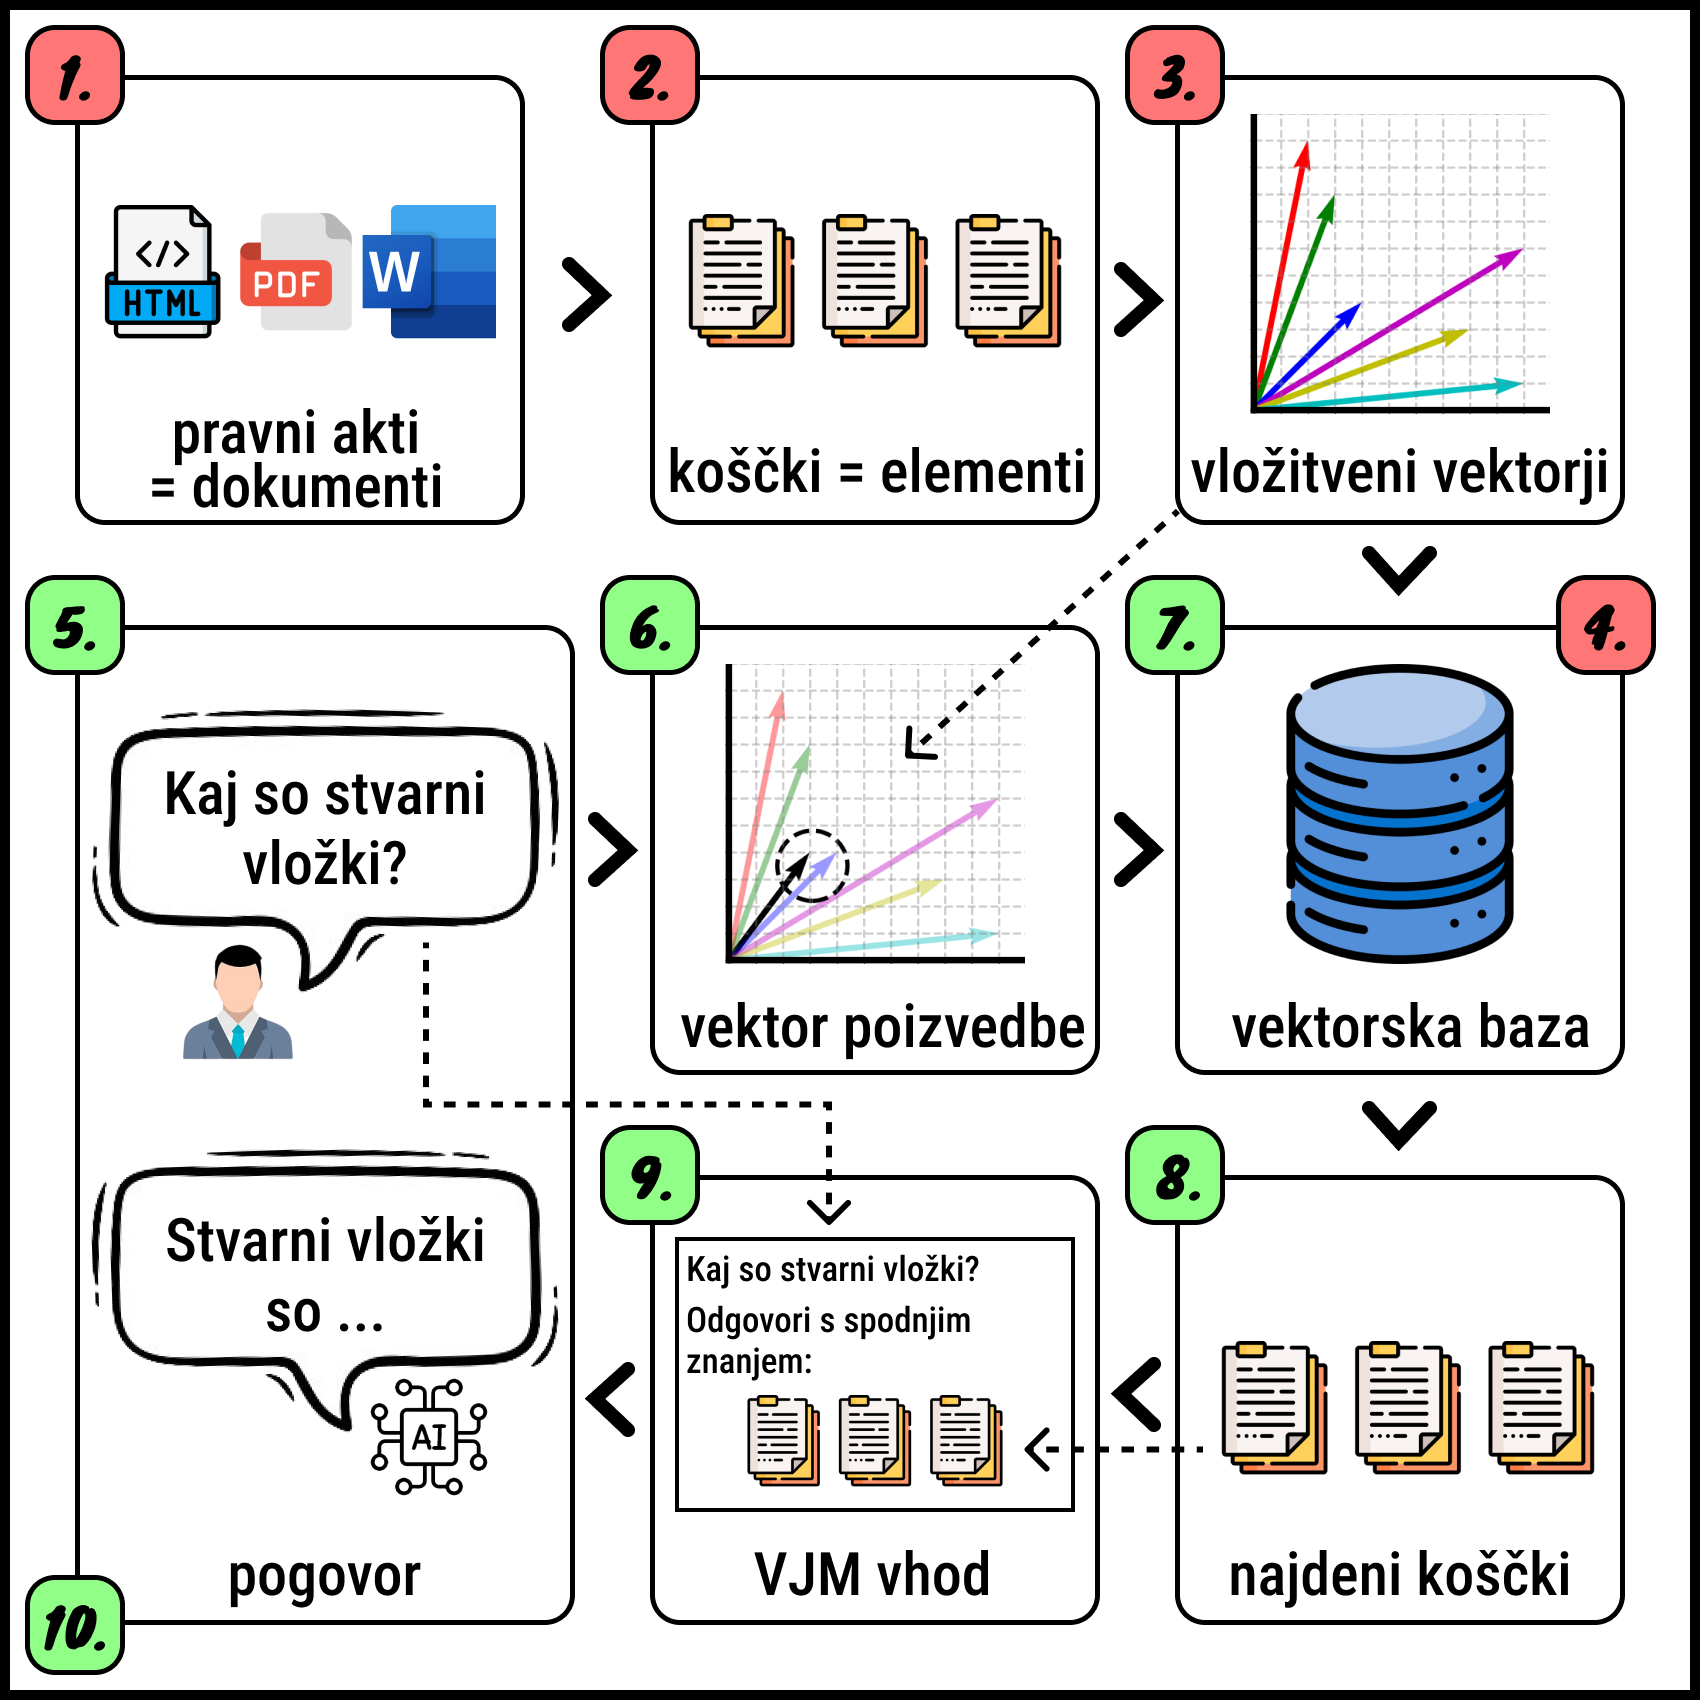
\includegraphics[width=\textwidth]{rag_shema.png}
	\caption{Shema RAG.}
	\label{rag_shema}
\end{figure}

Izbira kodirnega modela, VJM-ja, vektorske baze in podobnega so parametri, ki vplivajo na uspešnost metod. V vseh metodah konsistentno uporabljamo enake parametre (jih fiksiramo), s čimer zagotovimo enako podlago za vse metode. Vsi uporabljeni modeli so podrobneje opisani v poglavju Implementacija.

\subsection{Prednosti uporabe RAG-a}

Tehnika RAG je preprosta v ideji, a močna v izvedbi. Čeprav še zmeraj obstajajo številni izzivi, RAG bistveno izboljša natančnost odgovorov in zmanjša halucinacije, predvsem na domenskem področju \cite{benchmarking_rag}.

Dve dodatni veliki prednosti uporabe RAG-a sta nadzor nad znanjem in transparentnost virov. Ker so podatki ločeni od VJM-ja, shranjeni v zunanji bazi, imamo popoln nadzor nad tem, kateri podatki so notri. Tako lahko na primer zastarele podatke umaknemo in smo prepričani, da bodo informacije v odgovoru vedno aktualne. Če bi bile te interni del VJM-ja, prek učenja ali dodatnega treniranja (angl. fine-tuning), nimamo nobenega nadzora, kako jih bo VJM uporabil, niti zagotovila, da so aktualne. Nadalje za vsako informacijo, ki jo podamo VJM-ju, vemo, od kod prihaja, je enostavno našteti vire, prek katerih lahko uporabnik preveri verodostojnost odgovora, ali pa si več prebere na to temo.

Zgoraj je opisan preprosti ali naivni RAG \cite{rag} (angl. naive RAG): najprej razdeli domenska besedila na manjše enote, nato pridobi vložitve, ko pride vprašanje, pa pridobi vložitev vprašanja in ga primerja z drugimi, da dobi vsebine, ki so najbolj semantično podobne vprašanju, in vprašanje skupaj z domenskim znanjem poda VJM-ju.

\subsection{Pomanjkljivosti naivnega RAG-a}

Drži, da že s tem, ko uporabimo naivni RAG, močno izboljšamo generiran odgovor, vendar ima naivni RAG številne pomanjkljivosti, med njimi so \cite{rag_survey}:

\begin{itemize}
	\item slabo zastavljeno vprašanje in nepomembne vsebine – če naredimo poizvedbo tako, da dobesedno primerjamo uporabnikovo zastavljeno vprašanje z vsebinami, lahko dobimo nepomembne vsebine, če je vsebina poizvedbe napačna.
	\item ponavljanje vsebin – nenatančna priprava podatkov lahko povzroči, da se v eni poizvedbi vrne več različnih tekstov z isto vsebino;
	\item vračanje vsebin – namesto, da besedila VJM poveže v smiselno celoto in s tem uporabniku odgovori na vprašanje, preprosto le parafrazira vsebine (kot papiga);
	\item halucinacije – vedno je nevarnost, da se VJM “odloči” ne upoštevati navodil in se ne zmeni za podane informacije ter poskusi odgovoriti iz internega znanja.
\end{itemize}

\subsection{Napredni RAG}

V ta namen se je razvila naprednejša tehnika: napredni RAG \cite{rag_survey} (angl. advanced RAG). Napredni RAG vzame temelje naivnega RAG-a in doda številne izboljšave.

Namesto da za poizvedbo uporabi uporabnikovo vprašanje takšno, kot je, ga najprej pretvori v primernejšo obliko. Obstaja več načinov, med katerimi sta najbolj razširjena razširitev poizvedbe in sprememba poizvedbe. Preden naredimo poizvedbo, razširimo uporabnikovo vprašanje in ga pretvorimo v primernejšo obliko. S tem dosežemo, da je poizvedba bližje končni iskani vsebini.

Naslednja velika sprememba se zgodi po tem, ko najdemo dokumente. Preden so dokumenti podani v VJM, jih še enkrat predelamo. Dokumente s ponovnim sortiranjem (angl. reranker) obdelamo tako, da so vsebine, ki bolje odgovarjajo na vprašanje, višje v rangirnem listu. Ponovno sortiranje deluje namreč tako, da za vhodno poizvedbo in najden dokument vrne, kako pomemben je dokument za poizvedbo \cite{query_rewriting}. Medtem ko v prvem koraku s kodirnikom vložimo poizvedbo in primerjamo semantično podobnost z drugimi dokumenti, tukaj primerjamo, kako je najdena vsebina pomembna za poizvedbo. Drobna, a pomembna razlika.

Še dva pogosta pristopa v tem delu sta povzetek in združevanje besedil (poleg ponovnega sortiranja) \cite{other_query_transformations}. Na področju prava ti tehniki izpadeta, saj bi parafrazacija ali izpuščanje zakonodaje hitro vodilo v napačno podane informacije. Vendar širša ideja za druga področja ostane ista: ko najdemo dokumente, jih predelamo na način, ki bo VJM-ju omogočil, da bo kar se da dobro odgovoril na uporabnikovo vprašanje.

Ta dva ključna dodatna dela, sprememba pred poizvedbo in sprememba po njej, močno izboljšata naivni RAG.

Vredno je omeniti, da ko pridobivamo podatke, je več poudarka predvsem na prvem koraku. “Garbage in garbage out” je ena izmed prvih fraz, ki jo vsak nadobudni podatkovni znanstvenik sliši. Izboljšava tega koraka seveda ni omejena na napredni RAG, saj enako močno velja za naivnega.

\subsection{Modularni RAG}

Najnovejša različica RAG-a je modularni RAG. Namesto fiksne strukture, kot jo imata naivni in napredni RAG, je tu vse modularno. Razvijalec za vsak primer sam presodi, katere komponente so najustreznejše.

Shematsko lahko module združimo v iskalne, spominske, preusmerjevalne, napovedovalne itd. Iskalni moduli omogočajo večjo fleksibilnost za specifične scenarije, kot so iskanje po različnih virih (vektorska baza, grafna baza, internet itd.), z možnostjo generiranja poizvedb in ustrezne poizvedene kode. RAG-Fusion spremeni omejitve ene perspektive, s tem da vzporedno naredi več poizvedb z različnih zornih kotov in pametnim ponovnim razvrščanjem, s čimer doseže boljšo prepletenost znanja. Preusmerjevalni modul se odloči za optimalno pot poizvedbe prek različnih virov poizvedbe in kako znanje iz različnih virov združiti nazaj skupaj \cite{rag_survey}.

Osnovna ideja ostane enaka: glede na uporabnikovo vprašanje najdemo najustreznejše dokumente, s katerimi VJM odgovori na uporabnikovo vprašanje. Vse drugo je variabilno; razvijalec/raziskovalec presodi, kateri moduli bodo za problem najustreznejši, in jih vstavi v cevovod RAG.

Po temeljitem pregledu literature nisem zasledil modularne implementacije RAG-a na področje prava. Zatorej predlagam novo arhitekturo, opisano v \hyperref[llm_kg_rag]{poglavju implementacije}.

Do zdaj je bilo implicitno dorečeno, da je vse zunanje znanje (tj. zakonodaja) shranjeno v vektorski bazi. Kot pa sem že v uvodu nakazal, je grafna baza veliko bolj primerna za shranjevanje povezav med entitetami, česar v zakonodaji ne primanjkuje.

Hu in sod. delijo metodi za generiranje jezika s predtreniranim VJM-jem z zunanjimi viri na (a) poizvedbene metode (RAG) in (b) grafno bazo. Znanje podgrafa vsebuje dodatne in poglobljene informacije določenega koncepta \cite{hu_survey}.

Konkretno to pomeni, da za določeno entiteto (npr. člen zakona) zraven vključimo še dodatne pomembne vsebine, kot so referencirani členi, uporabljene definicije itd.

\section{Sorodni projekti}

\subsection{PISRS}

Pravno-informacijski sistem Republike Slovenije \cite{pisrs} je “de facto” spletišče za pravnike. Vsebuje celotno slovensko zakonodajo, sodno prakso, evropsko zakonodajo itd. Poleg dostopa do dejanskih datotek pravnih aktov ponuja številne druge uporabne storitve, kot so:

\begin{itemize}
	\item neuradna prečiščena besedila – za vsak zakon je na spletišču dostopno neuradno prečiščeno besedilo; kakršnikoli popravki ali morebitne spremembe v drugih aktih, ki spreminjajo določen zakon, so vidni v predogledu;
	\item povezava do sodne prakse – vsak sodni primer, ki se nanaša na kakšno določbo iz zakona, je naštet;
	\item podatek o veljavnosti akta – ali je pravni akt veljaven ali ne;
	\item povezave med akti – povezave do drugih aktov, ki vplivajo ali posegajo v besedilo; to so razni popravki zakonov ipd.
	\item pravna podlaga in podrejeni akti – iz česa izvira ta pravni akt in kateri drugi pravni akti so napisani na podlagi tega akta;
	\item napredno iskanje – možnost iskanja po naslovih ali vsebini, vrsti pravnega akta, času objave v uradnem listu, identifikacijski številki itd.
\end{itemize}

Kot vidimo, ponuja pravno-informacijski sistem pester nabor funkcionalnosti. Ni pravnega delavca, ki ne bi uporabljal PISRS. Vendar je treba poudariti, da je to le iskalnik in ne vsebuje nobenih naprednih rešitev, kot je umetna inteligenca. Primer izgleda spletnega portala si lahko ogledate na sliki \ref{pisrs}.

Za vse, kar ponuja, pa ne ponuja pogovora z velikim jezikovnim modelom, ki bi se vedel kot pravni strokovnjak. Prav tako je iskanje po vsebini omejeno na ključne besede in ne omogoča semantičnega iskanja.

\begin{figure}[htbp]
	\centering
	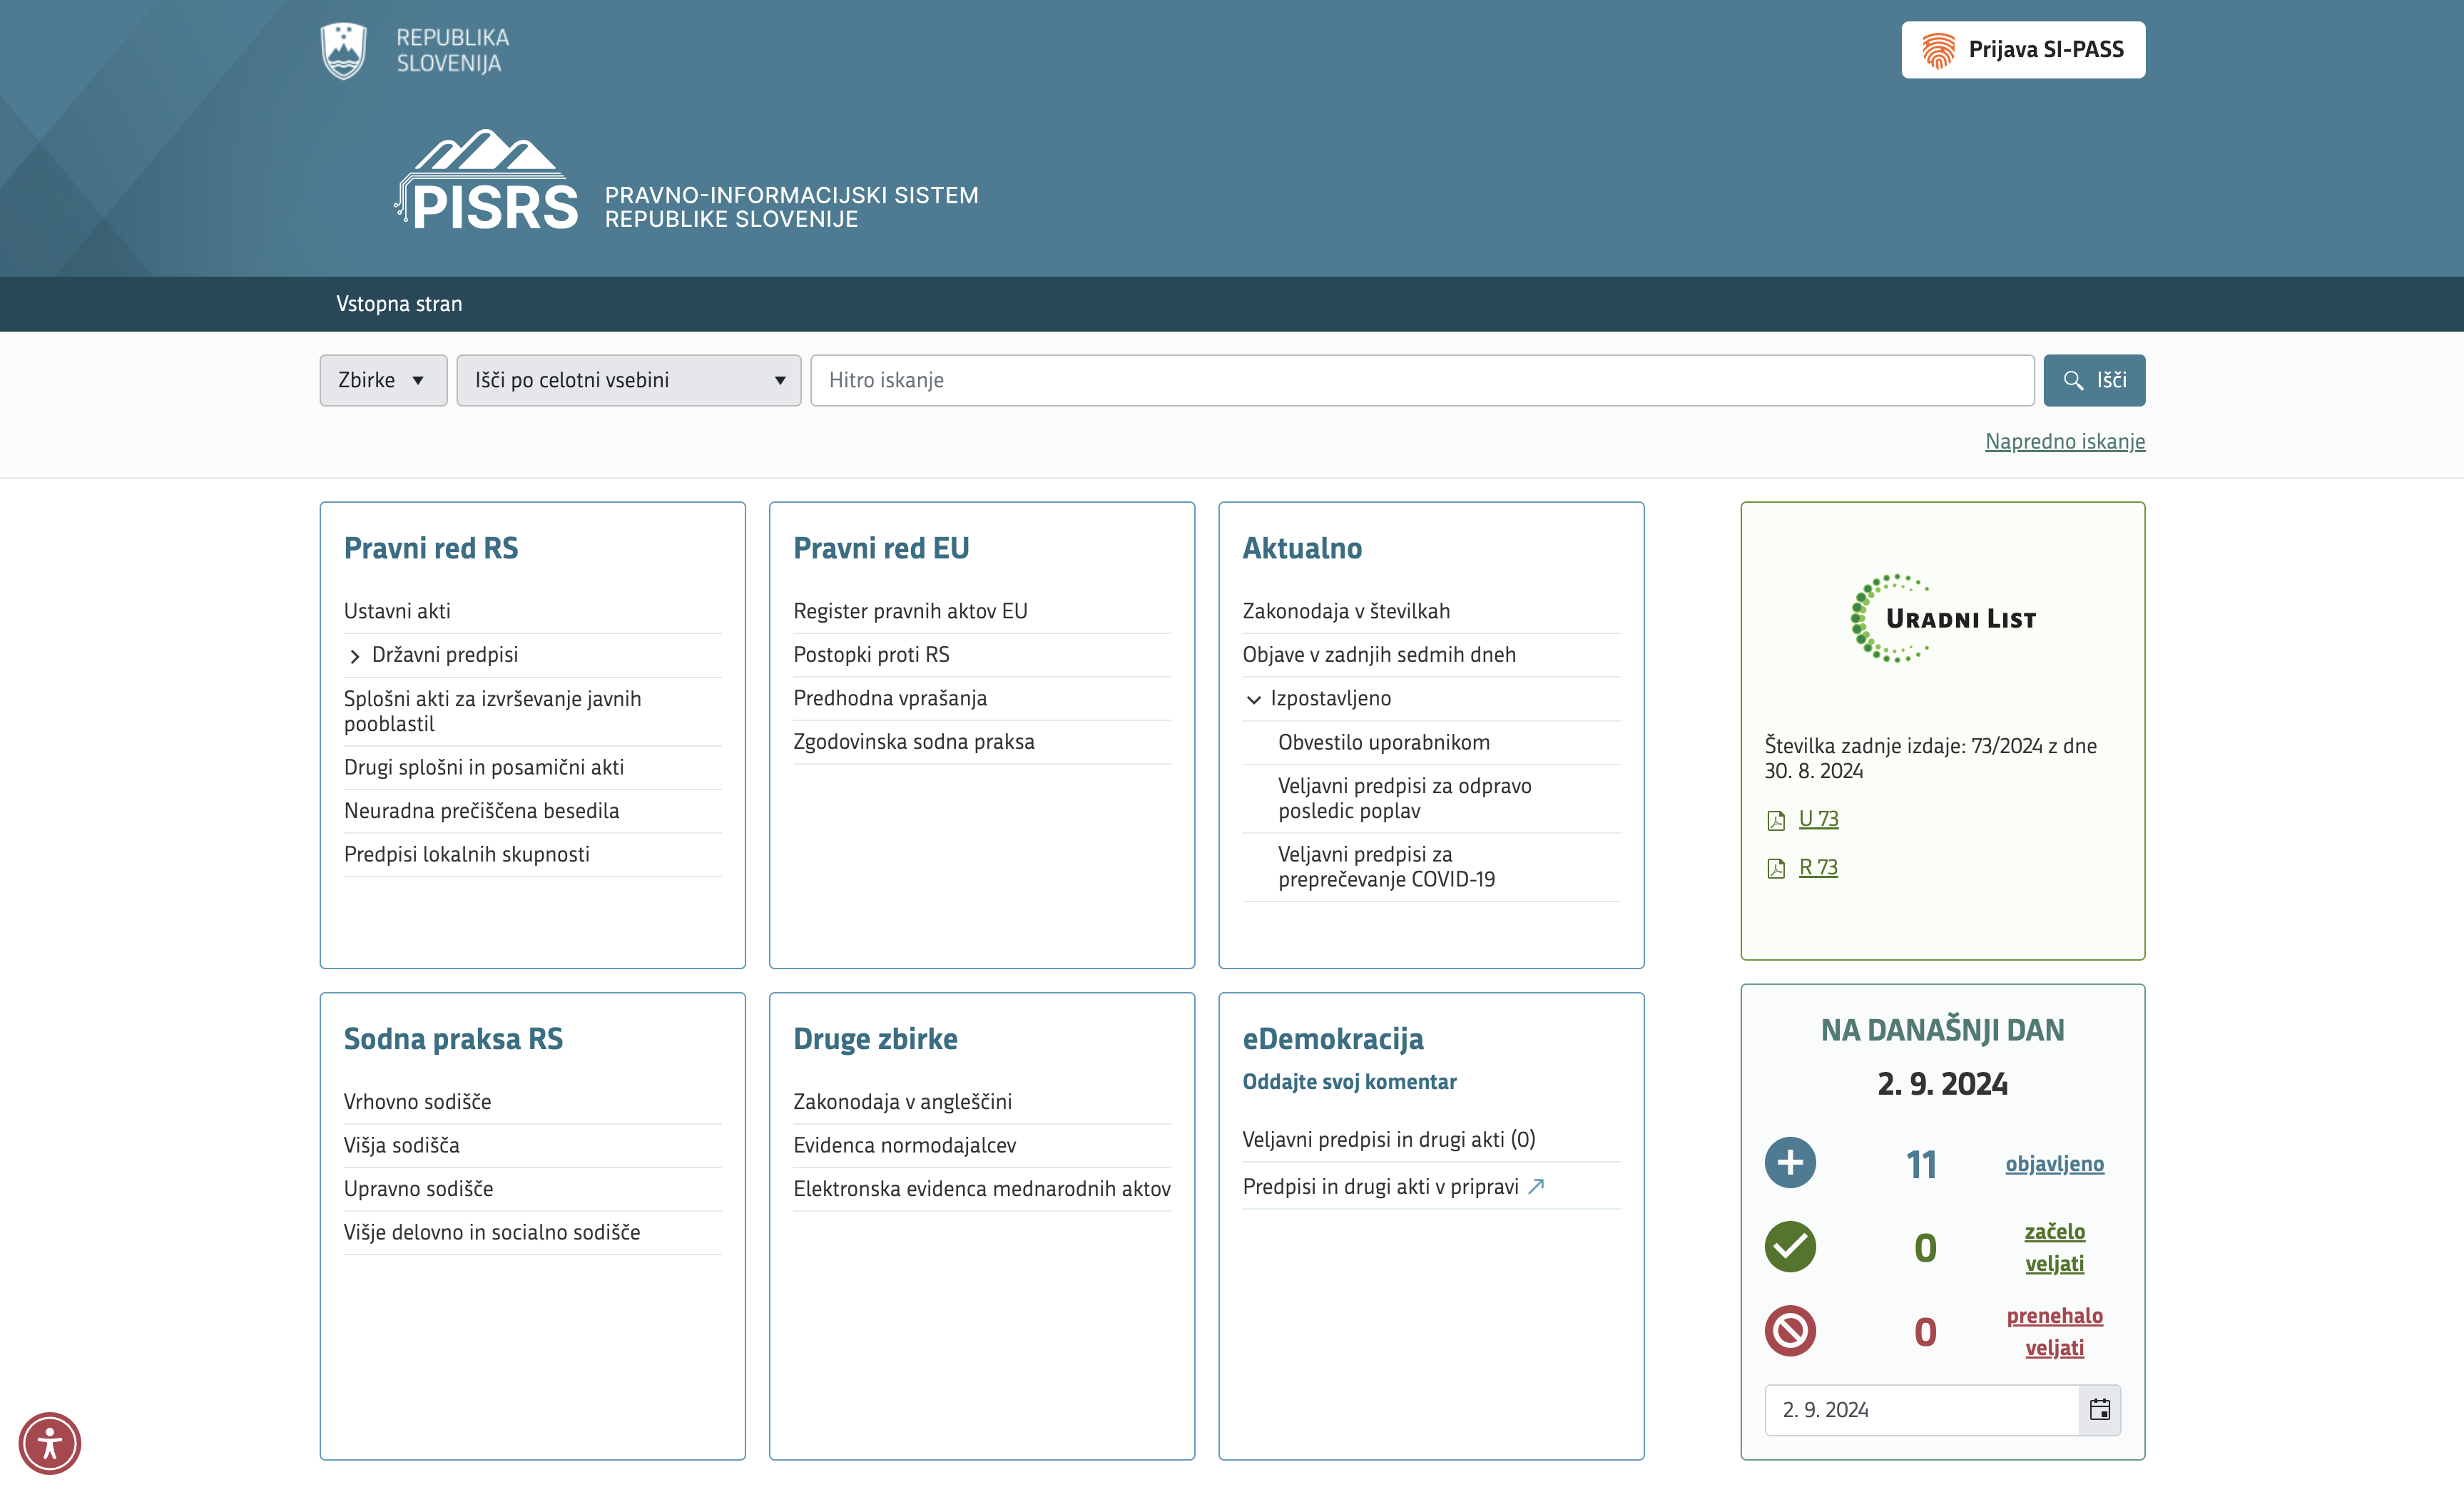
\includegraphics[width=\textwidth]{pisrs.png}
	\caption{Zaslonska maska spletnega portala PISRS.}
	\label{pisrs}
\end{figure}

\subsection{Pravko}

Pravko \cite{pravko} je podoben projekt našemu projektu. Gre za veliki jezikovni model, ki je strokovnjak na področju prava. Glede na informacije na spletišču

\begin{itemize}
	\item razume vprašanja v pogovornem jeziku,
	\item poišče uradne vire za odgovor,
	\item preišče vire in poda najverjetnejšo rešitev ter
	\item vrne uradne vire za nadaljnje raziskovanje.
\end{itemize}

Žal implementacijskih podrobnosti ne vemo, vendar ključne komponente delujejo podobno kot pri našem projektu. Za razumevanje pogovornega jezika se najverjetneje uporablja sprememba poizvedbe (angl. query transformation), za iskanje vsebin pa semantično iskanje. Vračanje uporabljenih virov na koncu je trivialno. Izgleda kot napredni ali modularni RAG. Primer uporabe Pravka si lahko ogledate na sliki \ref{pravko}.

Zdi se nam, da je Pravko uspešnejša implementacija glede na naše metode. Primerjavo naših metod s Pravkom lahko najdete na koncu poglavja o vrednotenju.

\begin{figure}[htbp]
	\centering
	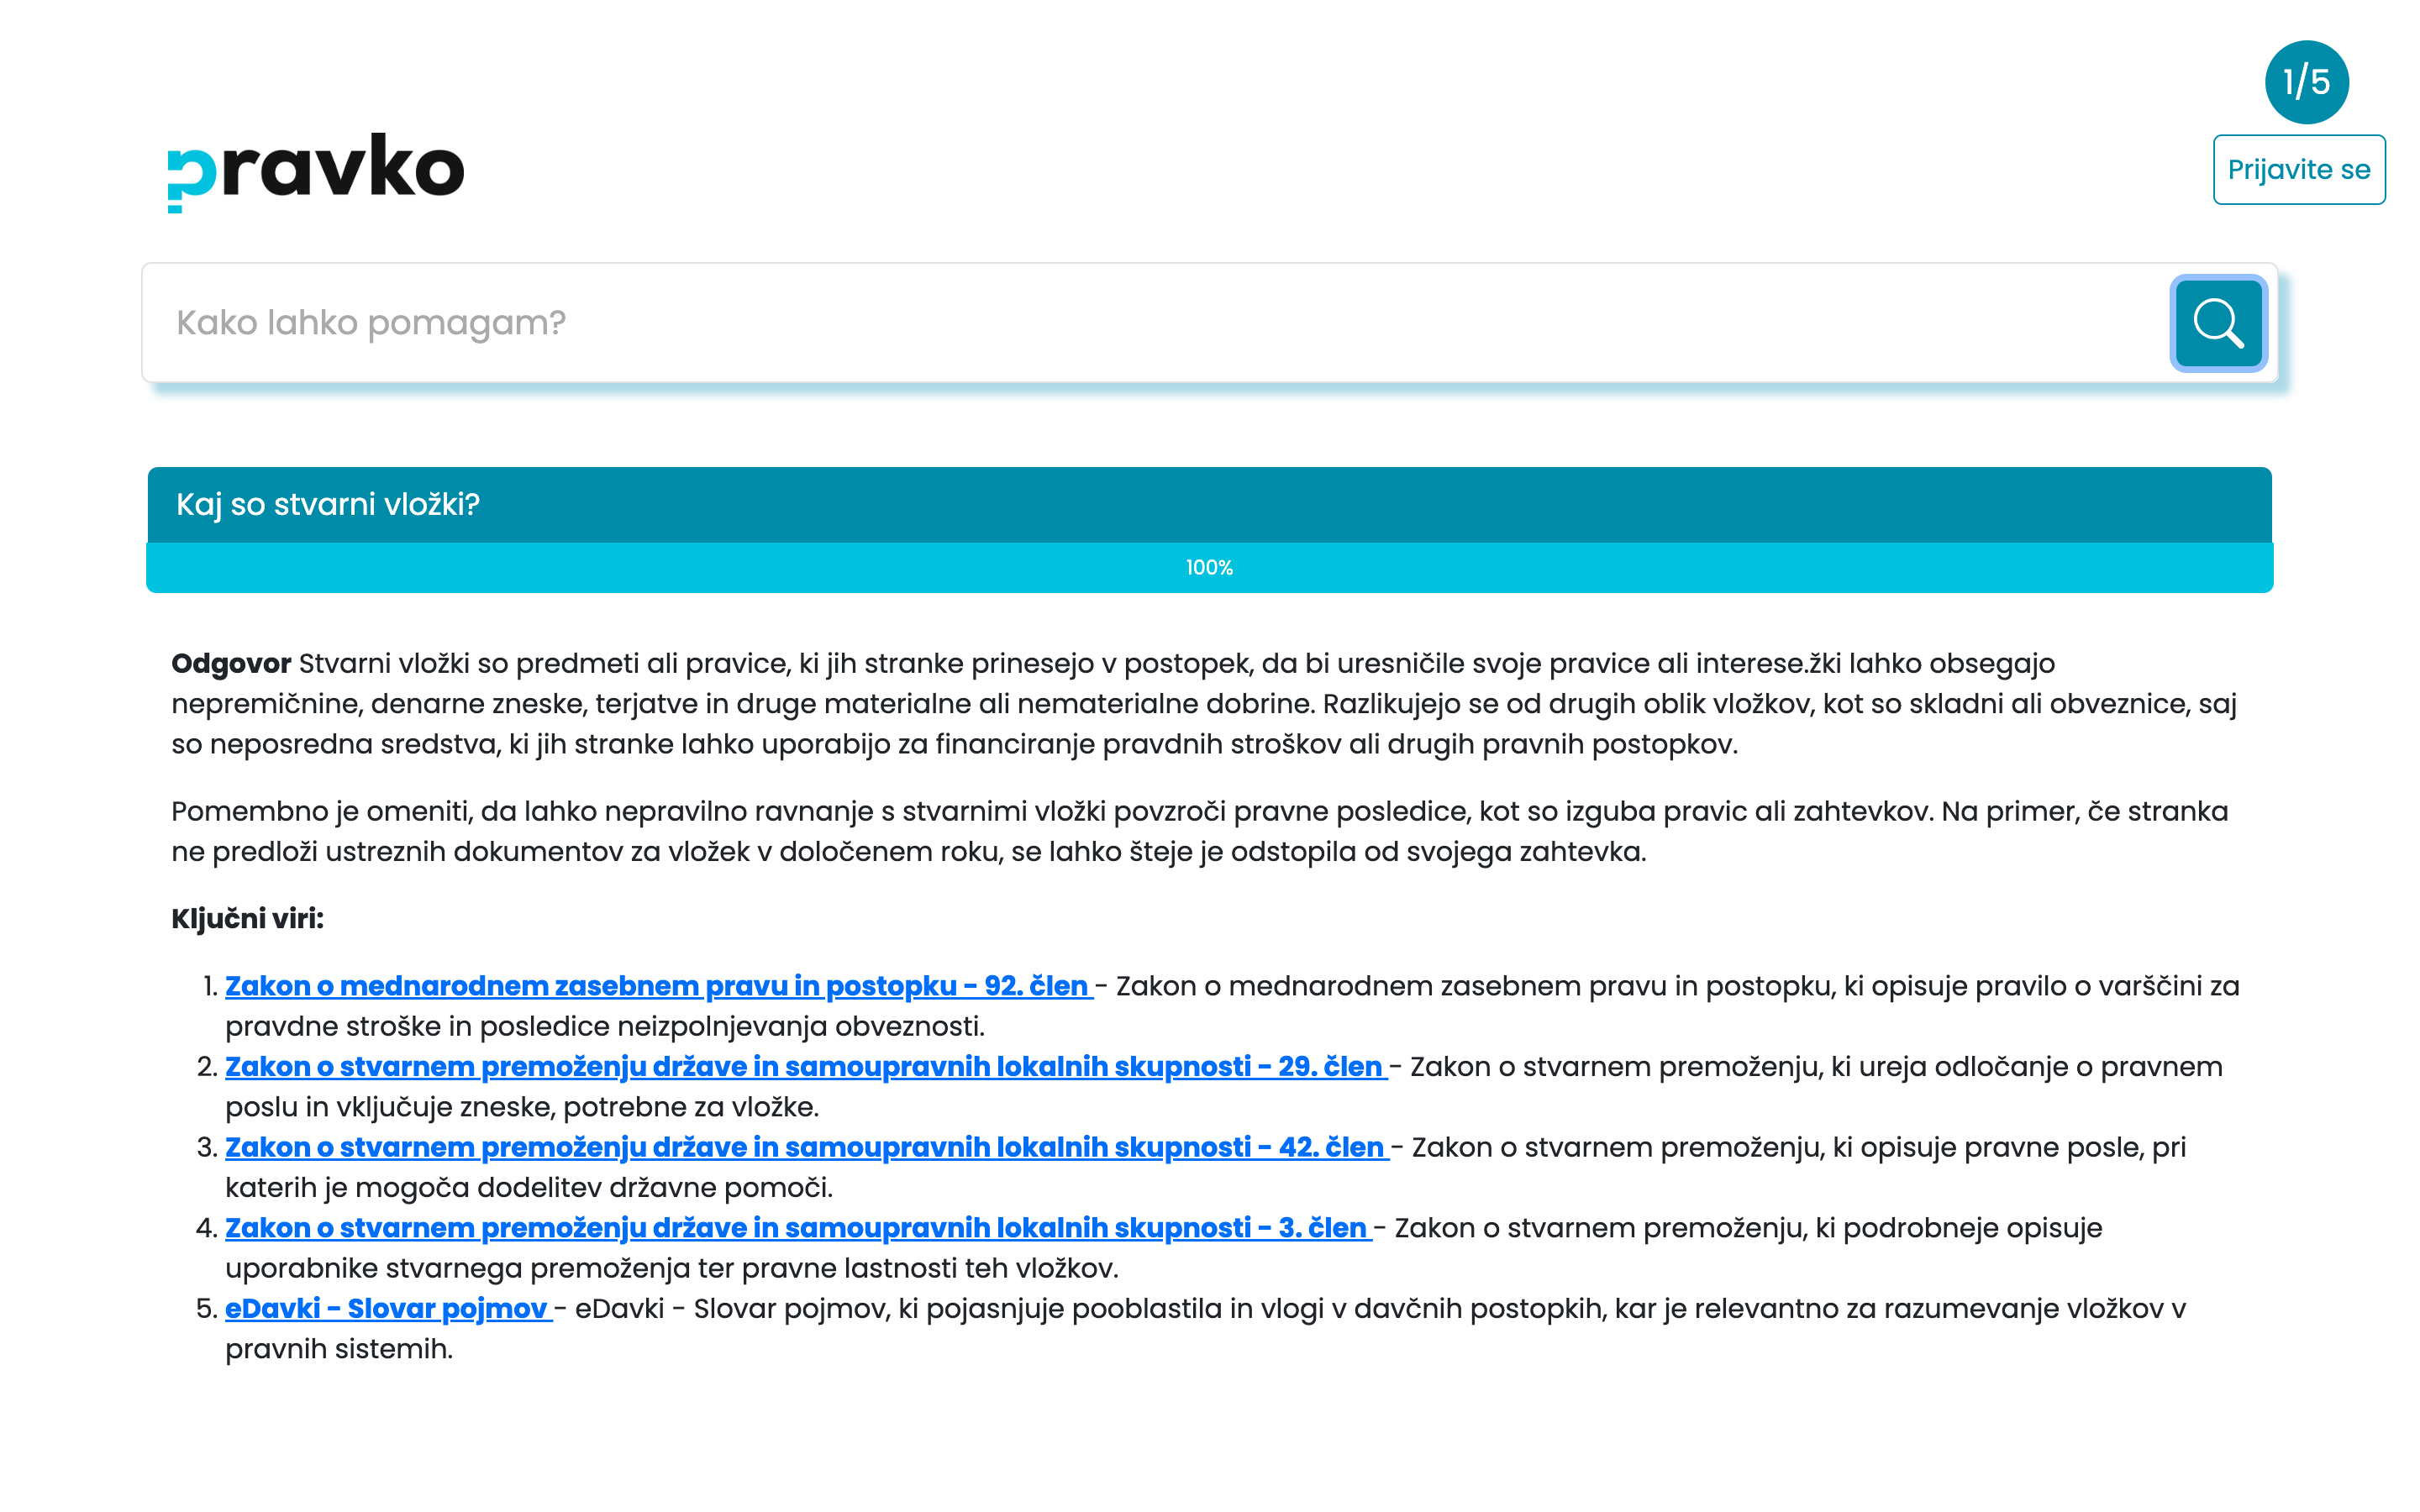
\includegraphics[width=0.9\textwidth]{pravko.png}
	\caption{Primer uporabe Pravka na spletni aplikaciji.}
	\label{pravko}
\end{figure}

\subsection{IUS-INFO}

IUS-INFO \cite{ius-info} je še eno spletišče za pravnike, ki se promovira kot “umetna inteligenca za pravnike”. Storitev je plačljiva in nimamo izkušenj z uporabo kot tudi ne drugih informacij glede implementacije, saj gre za zaprto rešitev, tako da razen omembe ne moremo narediti nadaljnje primerjave. Primer iskanja po spletnem portalu si lahko ogledate na sliki \ref{ius_info}.

\begin{figure}[htbp]
	\centering
	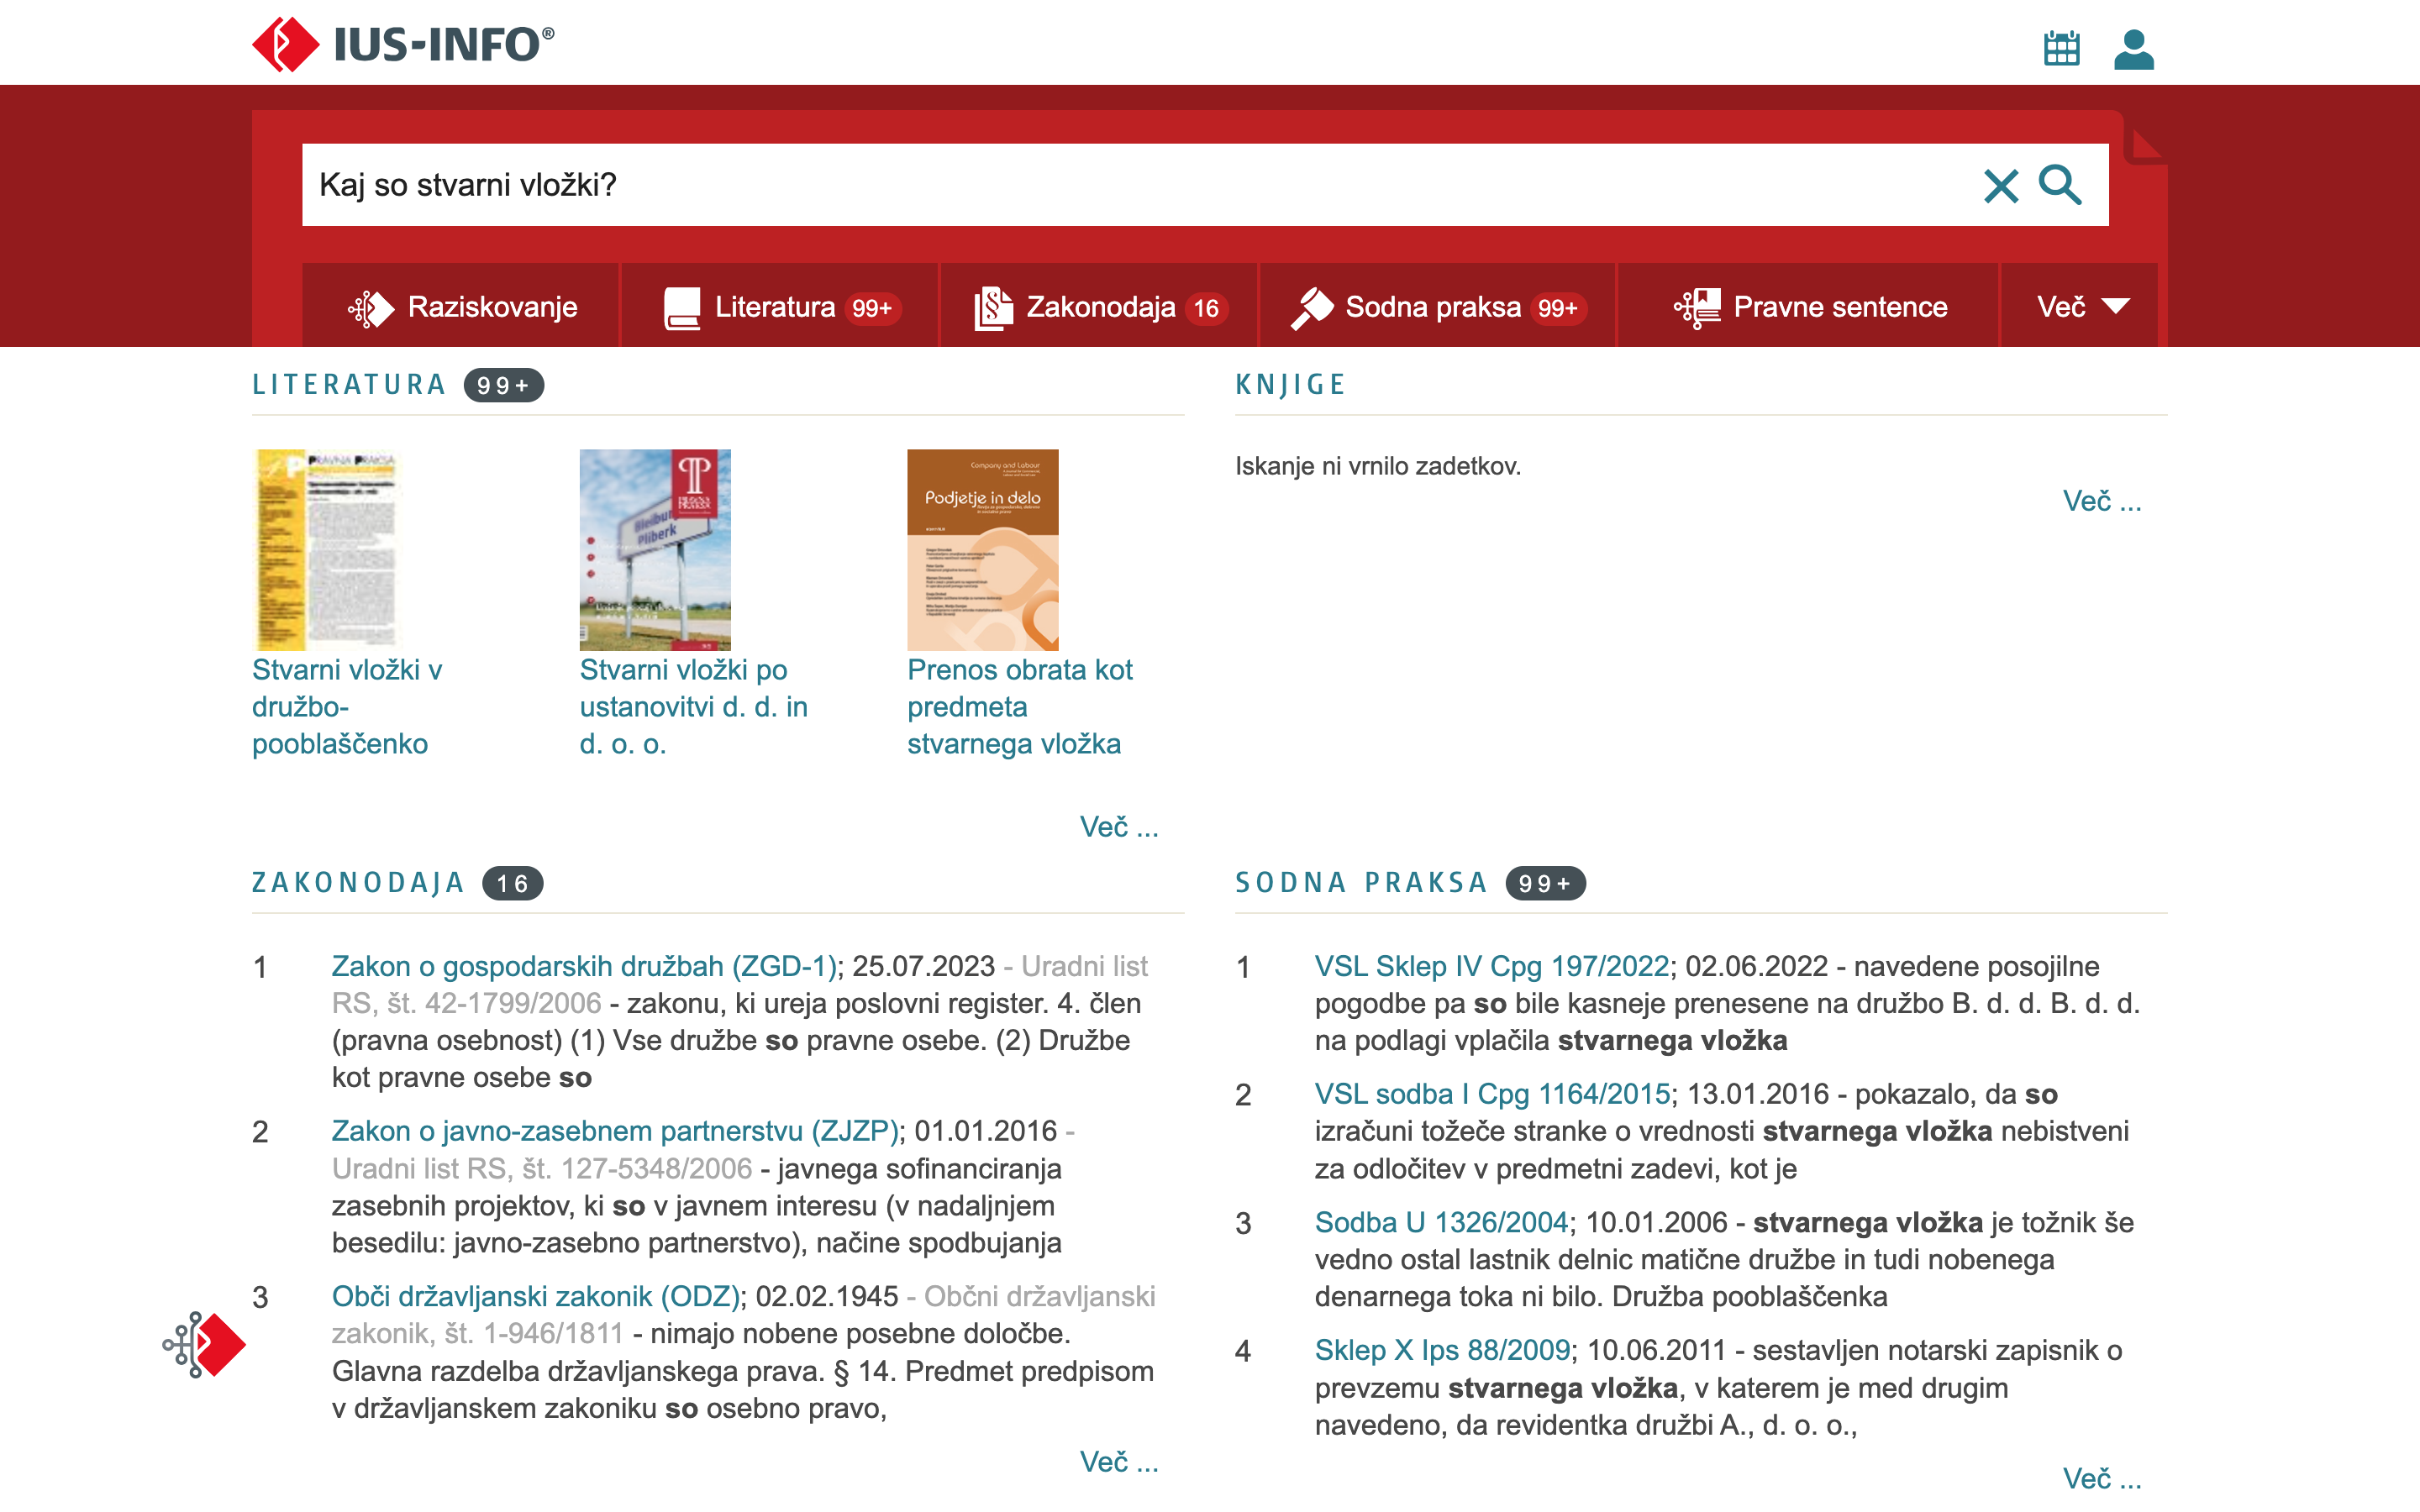
\includegraphics[width=0.9\textwidth]{ius-info.png}
	\caption{Primer iskanja po spletnem portalu IUS-INFO.}
	\label{ius_info}
\end{figure}

\clearpage

\subsection{ChatLaw}

ChatLaw \cite{chatlaw} je podoben projekt našemu projektu. Na področju kitajskega prava so želeli razviti sistem, ki je sposoben odgovarjati na poljuben pravni problem in se pogovarjati o poljubnih pravnih temah. Arhitektura je podobna, a bolj napredna in sofisticirana, kot je v do zdaj opisanih primerih.

Chatlaw je ekipa agentov, kjer ima vsak svojo vlogo. Agent je specializiran VJM, ustvarjen z namenom, da reši specifično težavo. Pogosto imajo agenti na voljo tudi orodja, ki jim omogočajo klicanje arbitrarnih funkcij \cite{agents}. Primer bi bil, da je orodje iskanje po vektorski bazi, kjer VJM poda iskalni niz. VJM se tako lahko odloči/presodi, kdaj bi bilo smiselno iskanje po bazi.

Chatlaw je sestavljen iz naslednjih agentov: svetovalec, raziskovalec, odvetnik in urejevalec. Vsi agenti so tudi posebna vrsta VJM-ja – mešanica strokovnjakov (angl. mixture of experts). Gre za posebno arhitekturo VJM-ja, ki je sestavljena iz več specializiranih enot in usmerjevalnika (router), ki glede na vhodni niz določi, kateri od strokovnjakov je najbolj sposoben odgovoriti na vprašanje. Arhitektura je vidna na sliki \ref{chatlaw}. Slika je vzeta iz članka ChatLaw-ja.

Svetovalec uporablja pogoste vzorce poizvedb v pravnih svetovanjih, da uporabnika iterativno vodi skozi fazo pridobivanja informacij. Iz teh informacij sproti sestavlja graf znanja, ki predstavlja uporabnikovo unikatno situacijo. Ta korak je analogen s preoblikovanjem poizvedbe.

Raziskovalec je pristojen za iskanje literature. Med iskanimi objekti so pravne entitete, povezave med njimi in pravni primeri. Vsak najden dokument je ponovno sortiran z uporabo VJM-ja. Ta korak je bržkone identičen koraku poizvedbe v naprednem RAG-u.

Odvetnik in urejevalec najdene vsebine predelata in vrneta uporabniku v ustrezni obliki (formi). Odvetnik pogleda najdene dokumente, se za vsakega odloči, ali je ustrezen za primer, in poveže znanje iz različnih virov v končni odgovor. Urejevalec vzame odgovor in ga pretvori v ustrezno obliko.

Vse komponente so dotrenirane na kitajskih pravnih dokumentih, kar izboljša pravno terminologijo agentov in učinkovitost iskalnika.

\begin{figure}[htbp]
	\centering
	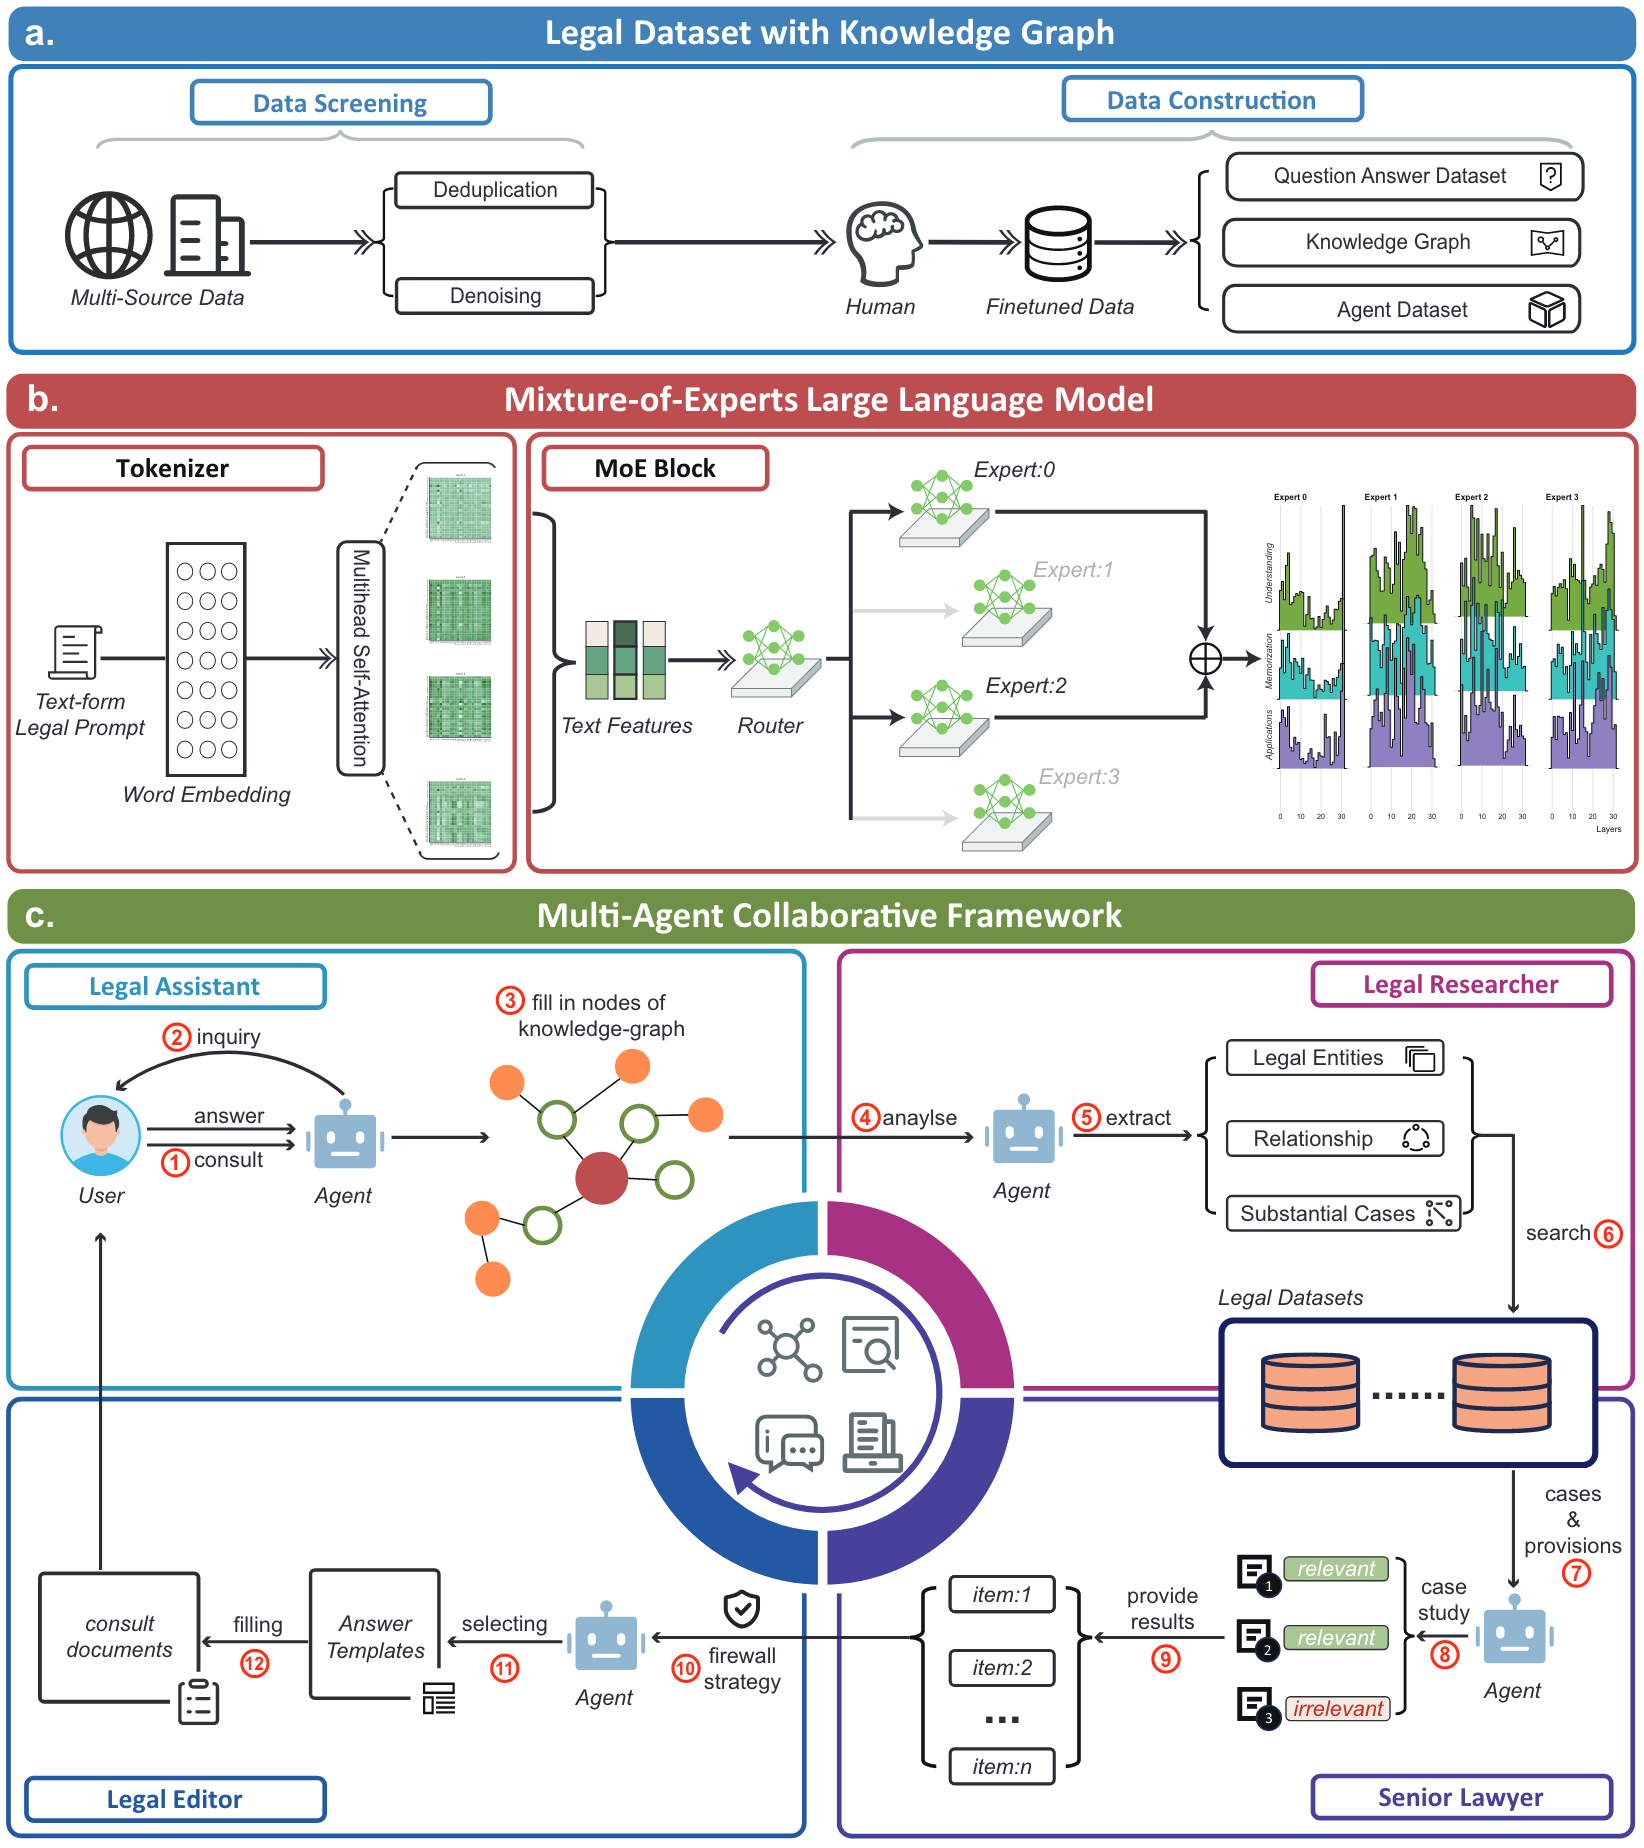
\includegraphics[width=\textwidth]{chatlaw.png}
	\caption{Arhitektura projekta ChatLaw.}
	\label{chatlaw}
\end{figure}

\chapter{Podatki}
\label{ch2}

Podatke delimo na dva sklopa: učno in testno množico. Učna množica je podmnožica slovenskih pravnih aktov, ki določajo obseg znanja velikega jezikovnega modela. V praksi to pomeni, katere akte bomo razkosali, vložili, indeksirali in med njimi vzpostavili povezave ter kateri akti bodo na voljo za iskanje. Testna množica pa so vprašanja, na katera se lahko odgovori z znanjem iz aktov iz učne množice.

\section{Zakonodaja}

Ker je vprašanje te diplomske naloge, kako efektiven je lahko VJM kot pravni svetovalec na področju slovenskega prava, se omejimo na slovensko zakonodajo.

Kot je bilo že rečeno v uvodu, obstaja vrsta različnih pravnih aktov. Vendar zaradi obsežnosti ni izvedljivo, da bi za namen te diplomske naloge lahko vso indeksirali.

Iz tega namena in želje, da lahko dobro definiramo metriko in testno množico, se bomo omejili le na eno pravno področje – gospodarsko pravo. V ta namen smo indeksirali vso zakonodajo, ki se nanaša na to področje. Zaradi omejenega števila razpoložljivih sredstev smo lahko indeksirali le ta del zakonodaje. Velik del vnosa zakonodaje je potekal ročno, predvsem vnos referenc, kar je zahtevalo veliko časa.

Referenčne povezave smo poskusili vzpostaviti avtomatsko s pomočjo VJM-ja, vendar modeli pri tej nalogi niso bili dovolj uspešni. Veliko označenih referenc je bilo lažno pozitivnih (angl. false positive), nekaj primerov je bilo tudi lažno negativnih (angl. false negative). Ni nam ostalo drugega, kot da reference vnesemo ročno. Ker je število referenc ogromno, nismo klasificirali vseh, vendar le del. V bazo smo shranili tiste, ki so se pojavile v vsebinah, ki so pomembne za odgovore na vprašanja.

Glavni sklopi pravnih aktov, ki so indeksirani, so

\begin{itemize}
	\item Zakon o gospodarskih družbah,
	\item Zakon o finančnem poslovanju, postopkih zaradi insolventnosti in prisilnem prenehanju,
	\item Zakon o revidiranju,
	\item Zakon o bančništvu,
	\item Zakon o zavarovalništvu,
	\item Zakon o prevzemih in
	\item Slovenski računovodski standardi.
\end{itemize}

Vsak sklop pravnih aktov vsebuje istoimenski (glavni) zakon in možne popravke tega zakona, odločbe ustavnega sodišča, ki se nanašajo na ta zakon, in druge zakone, ki se nanašajo na ta zakon. Osnovne statistike so na voljo v tabeli \ref{statistika}.
\begin{table}[htbp]
	\centering
	\begin{tabular}{|l|c|}
		\hline
		Statistika                                & Vrednost \\ \hline
		št. dokumentov oz. pravnih aktov          & 44       \\ \hline
		št. (osnovnih) zakonov                    & 13       \\ \hline
		št. popravkov zakona                      & 25       \\ \hline
		št. odločb ustavnega sodišča              & 6        \\ \hline
		skupno št. pravnih členov v pravnih aktih & 4422     \\ \hline
		povpr. št. pravnih členov / pravni akt    & 100      \\ \hline
		povpr. št. besed / člen                   & 113      \\ \hline
	\end{tabular}
	\caption{Statistika indeksiranih podatkov.}
	\label{statistika}
\end{table}

Kot je bilo omenjeno, smo indeksirali le del celotne slovenske zakonodaje. Celotna slovenska zakonodaja je veliko obsežnejša kot le področje gospodarskega prava. Vendar ker so pravna področja med sabo praviloma povsem izolirana, z izpustitvijo drugih pravnih aktov naša analiza ni pomanjkljiva. Vsa testna vprašanja so s področja gospodarskih družb. Vsa gospodarska zakonodaja je indeksirana in na voljo tehnikam RAG. Ker se vsa preostala zakonodaja, ki ni indeksirana, kot je npr. Zakon o pomorstvu ali Zakon o gradbeništvu, ne nanaša na gospodarsko področje, jo s semantičnim iskanjem metode ne najdejo (ostaja možnost, a so drugi zakoni vsebinsko povsem različni, zaradi česar je ta verjetnost izjemno nizka). Torej indeksiranje preostale zakonodaje ne vpliva na delovanje metod, kar je še dodaten razlog, da je ne indeksiramo.

Trditve v prejšnjem odstavku niso povsem resnične in potrebujejo nadaljnjo razlago. Če bi indeksirali še več zakonodaje, bi lahko videli (negativen) vpliv na uspešnost metod. Ker obstaja možnost, da bi se za poizvedbo vseeno našel del zakona, ki ga nismo indeksirali, bi to v metode vneslo šum. Pojavile bi se informacije, ki niso pomembne za odgovor na vprašanje. V naprednem in modularnem RAG-u bi ponovno sortiranje to težavo praviloma razrešilo, v naivnem RAG-u pa ne. Zaključimo lahko, da bi prisotnost dodatne zakonodaje negativno vplivala na naivni RAG, na napredni in modularni RAG pa ne (če model za ponovno sortiranje dobro opravi svoje delo). Na metodo, ki uporablja le VJM brez tehnike RAG, te razlike seveda ne vplivajo.

Da si bo bralec lažje predstavljal količino obdelanih podatkov, bomo prikazali še nekaj statistik, ki veljajo za celotno slovensko zakonodajo \cite{pisrs_stats}: vsega skupaj v Republiki Sloveniji velja 1.969 zakonov in 6.014 podzakonskih aktov. Podzakonski akti so derivacija zakonov, pogosto zaradi želje večje natančnosti na točno določenem področju (zakoni so bolj splošni). Primeri podzakonskih aktov so uredbe, pravilniki, odloki itd. Kot je razvidno, smo indeksirali le majhen del celotne zakonodaje. S tem so naše metode omejene na znanje le s področja gospodarskega prava. Za splošnega pravnega asistenta bi bilo treba indeksirati celotno zakonodajo.

Vse zakone je možno dobiti v obliki PDF na pravno-informacijskem sistemu Republike Slovenije \cite{pisrs}.

Vsak zakon je sestavljen iz več poglavij in podpoglavij, od katerih ima vsak enega ali več členov. Člen je osnovna strukturna enota, ki celovito zajema en pojem.

\section{Testna množica}

Da bi lahko primerjali uspešnost različnih implementacij, smo določili 4 testne scenarije:

\begin{itemize}
	\item \textbf{Specifično vprašanje}: natančno zastavljeno vprašanje v pravni terminologiji, kjer so vse informacije na dosegu roke. V praksi to pomeni, da iz zakona vzamemo neko trditev, primer, definicijo ipd. in iz nje postavimo vprašanje. Vse informacije, potrebne za pravilen odgovor, so v celoti omejene na del besedila, v katerem se nahajajo (npr. točka ali alineja člena).
	\item \textbf{Specifično vprašanje z referencami}: enako kot zgoraj, a z eno razliko: v besedilu so omenjene vsebine drugih členov. Ko zakon bere dejanska oseba, ne računalniški sistem, in v besedilu piše “v skladu s prvim odstavkom 42. člena tega zakona”, bo pogledala to dodatno vsebino, da lahko bolje in v celoti razume določilo. Tako naivni kot napredni RAG imata to pomanjkljivost, da tem referencam ne sledita, zaradi česar ima VJM pomanjkljiv kontekst. Uporaba grafne baze bi morala rešiti ta problem.
	\item \textbf{Splošno vprašanje}: medtem ko sta zgornja dva scenarija omejena na primere, ko so vse informacije lokalno dostopne, pri splošnem vprašanju ni tako. Tu preverjamo zmogljivost programa, da najde pomembne informacije iz več različnih mest zakona in jih smiselno poveže v odgovor. Vprašanje je še vedno postavljeno v pravni terminologiji.
	\item \textbf{Konkretni primer}: nazadnje se še preverja učinkovitost sistema za vsakodnevnega uporabnika. Vprašanje je zdaj opis primera v vsakodnevnem jeziku, ki mu sledi dejansko vprašanje. Tu se primerja še, kako učinkovito lahko sistem nadomesti pravno osebo (v nekem smislu tolmača) v postopku.
\end{itemize}

Vsi testni primeri so omejeni le na obdelano literaturo, tj. Zakon o gospodarskih družbah.

Ker nismo našli javno dostopne testne množice, ki bi preverjala vse želene kriterije, smo testno množico sestavili sami v sodelovanju s strokovnjaki na tem področju.

Imeli smo izbiro med manjšim številom kakovostnih testnih primerov in večjim številom manj kakovostnih testnih primerov. Po posvetovanju smo se odločili za manjše število visoko kakovostnih testnih primerov. Ker želimo preveriti, ali bi se veliki jezikovni modeli kot pravni svetovalci lahko uporabljali v kritičnih sistemih, je bolj pomembno, da smo prepričani, da dobro delujejo na primerih, ki se dejansko pojavijo v praksi in niso le umetno postavljeni.

Z manjšim številom primerov nam je tudi uspelo uresničiti ročno ocenjevanje generiranih odgovorov, česar v primeru velikega števila testnih primerov ne bi bilo mogoče. Zaradi potrebnega domenskega znanja nam človeška presoja veliko bolje osvetli uspešnost metod kot računalniške metrike. To nam omogoči, da lahko veliko bolj realno ocenimo uspešnost metod.

Pomanjkljivost manjšega števila testnih primerov je, da obstaja nevarnost, da ne ocenimo metod na zadostnem številu podatkov in da testna množica ni reprezentativen vzorec. To težavo smo zmanjšali tako, da smo s testnimi primeri pokrili čim večji spekter vsebine.

Za vsak scenarij smo tako pripravili 10 parov vprašanje-odgovor, kar skupaj nanese 40 parov. Vsa vprašanja so na voljo v \hyperref[appendix_a]{Dodatku A}.

V tabeli spodaj smo zbrali nekaj statistik za vsakega od scenarijev:

\begin{table}[H]
	\centering
	\caption{Statistike testnih podatkov glede na scenarij.}
	\begin{tabular}{|c|c|c|c|c|}
		\hline
		statistika                & scenarij 1 & scenarij 2 & scenarij 3 & scenarij 4 \\ \hline
		št. vprašanj              & 10         & 10         & 10         & 10         \\ \hline
		povpr. št. besed/vpr.     & 11         & 8          & 9          & 19         \\ \hline
		povpr. št. žetonov/vpr.   & 23         & 20         & 20         & 40         \\ \hline
		povpr. št. besed/odg.     & 38         & 102        & 139        & 125        \\ \hline
		povpr. št. žetonov/odg.   & 89         & 244        & 333        & 302        \\ \hline
		št. koščkov               & 0          & 329        & 3271       & 3271       \\ \hline
		povpr. št. besed/košček   & 0          & 273        & 32         & 32         \\ \hline
		povpr. št. žetonov/košček & 0          & 644        & 74         & 74         \\ \hline
	\end{tabular}
\end{table}

Za vsak scenarij si spodaj lahko ogledate primer vprašanja (nekateri odgovori so dokaj dolgi, zato so zaradi preglednosti izpuščeni); vsa preostala vprašanja si lahko ogledate v \hyperref[appendix_a]{Dodatku A}:

\begin{enumerate}
	\item Na podlagi česa se določi sistem vodenja poslovnih knjig podjetnika?
	\item Za katere družbe slovenski računovodski standardi ne določajo vsebine konsolidiranega letnega poročila?
	\item Kako vodijo poslovne knjige družbe, ki se po velikostnih kriterijih razvrščajo med velike družbe?
	\item Sem samostojni podjetnik posameznik in sem dejavnost prenesel na ženo. Je to mogoče? Kaj moram storiti?
\end{enumerate}

\chapter{Implementacija}
\label{ch3}

Kot je bilo že omenjeno v pregledu literature, bomo primerjali 4 različne metode, kjer je vsaka različica naprednejša od prejšnje.

Veliki jezikovni model, ki ga uporabljamo v vseh metodah, je kvantiziran Gemma 2 (gemma2:9b-instruct-q6\_K) \cite{gemma2}. Razlog kvantizacije je hitrejše generiranje in možnost uporabe modela na naši grafični kartici (Apple M3 Max). Po krajšem testiranju s preostalimi modeli smo ugotovili, da se ta model najbolje odziva na ukaze (pomembno za RAG, saj mora model slediti navodilom, da na vprašanje odgovori iz najdenega znanja) ter najbolje razume in generira slovenski jezik. Testiranje je potekalo ročno in je bilo večinoma odvisno od subjektivne ocene ocenjevalcev. Za naše potrebe se je Gemma 2 izkazal kot najprimernejši kandidat za VJM.

Veliko modelov je zmogljivejših, a še več jih ima pomanjkljivost nerazumevanja slovenskega jezika, zaradi česar nam ne koristijo. Odločili smo se za odprte modele, zaprtih, kot so GPT-4 in Claude 3, nismo preverjali. Ker se lahko v praksi v vprašanjih, ki jih postavimo tem modelom, pojavijo osebne informacije, je zasebnost ključnega pomena. Odprti modeli nam omogočajo popoln nadzor nad podatki in vse osebne informacije ostanejo osebne, zato zaprtih modelov, kjer bi osebne podatke morali posredovati tujim podjetjem, ne obravnavamo.

Vsa izvorna koda je javno dostopna na \href{https://github.com/pizdoponi/diploma}{GitHub repozitoriju}: \\(\textit{https://github.com/pizdoponi/diploma}).

\section{VJM}

Ta pristop služi za izhodiščno točko. VJM-ju se iz testne množice postavi vprašanje brez dodatnih navodil ali konteksta. VJM mora tako iz internega znanja odgovoriti na vprašanje.

Največji pomanjkljivosti sta seveda pomanjkanje znanja (če slovenska zakonodaja ni bila v množici učnih podatkov), zaradi česar lahko model začne halucinirati, in aktualnost podatkov.

Navodilo, ki ga VJM dobi, se glasi:

\begin{verbatim}
    Si pravni pomočnik.
    Uporabnik ti bo postavil vprašanje.
    Nanj odgovori po najboljših zmogljivostih.
\end{verbatim}

\section{VJM + naivni RAG}

Zakon o gospodarskih družbah razčlenimo na manjše enote, tj. koščke (angl. chunks), fiksne dolžine (512 žetonov) in za vsako posebej izračunamo vložitveni vektor s kodirnikom. Zakon razčlenimo naključno, za kriterij delitve vzamemo znak za prelom vrstice. Razlog, zakaj zakon razdelimo na manjše dele, je večstopenjski. Kot prvo imata oba, kodirnik in veliki jezikovni model, omejeno število žetonov, ki jih prejmeta na vhodu. Celoten zakon se tako ne more procesirati v enem koraku. Kot drugo je problem preveč konteksta – če iščemo informacijo, ki je v enem odstavku, a imamo za enoto celotno poglavje, bo vložitveni vektor poglavja mnogo bolj splošen in drugačen od vektorja odstavka. Nastopita težavi, in sicer da ustreznega besedila ne najdemo ali da ima VJM preveč informacij in mu ne uspe izluščiti potrebnih.

Vektorje shranimo v vektorski bazi. Za vektorsko bazo uporabljamo odprtokodno bazo, imenovano Chroma \cite{chroma}. Chroma je učinkovita in praktična vektorska baza, ki je nastala izključno zaradi shranjevanja vektorjev in hitrega poizvedovanja po shranjenih vektorjih. Uporabljamo jo zaradi njene učinkovitosti, preprostosti uporabe in odprte kode (zaradi česar jo lahko uporabljamo lokalno).

Vsi vložitveni vektorji so pridobljeni s kodirnikom multiligual-e5-large \cite{multilingual-e5-large}. Gre za kodirnik, zgrajen na arhitekturi SBERT-a oz. transformerja stavkov (angl. sentence transformer) \cite{sbert}. Ta kodirnik je bil v času pisanja tega dela najvišje uvrščeni večjezični (podpora slovenščine je ključna) kodirnik z manj kot 500 milijoni parametrov na lestvici kodirnih modelov \cite{mteb}. Izbrali smo ga zaradi kombinacije uspešnosti (najvišja uvrstitev v zahtevanih pogojih) in hitrosti (majhno število parametrov).

V primerjavi z navadnim kodirnikom, kot ga poznamo iz transformerja, se tu vzporedno uporabljata dva identična kodirnika, ki ju naučimo prepoznavati, katera vhodna besedila so si podobna in katera ne. Ta premik perspektive omogoča modelom, da veliko bolje razlikujejo, katere vsebine so si sorodne; kar je ključno, saj tako lahko za vhodno poizvedbo zanesljivo najdemo del besedila, ki je podoben tej poizvedbi (pri predpostavki, da nam ta podobnost nudi informacije za odgovor na poizvedbo).

Ker uporabljamo slovenski jezik, uporabljamo tudi večjezično različico transformerja stavkov \cite{multilingual-sbert}. Gre za razširitev enojezičnih transformerjev stavkov na večjezične.

Ta pristop je enostaven, a pomanjkljiv. Ker ne delimo besedila glede na strukturo niti ne na semantiko, ampak na določene znake, obstaja nevarnost, da se pomembna vsebina ne nahaja na istem mestu. Primer: člen razdelimo na polovici, s čimer nimamo na voljo celotne vsebine člena, ko najdemo eno od polovic.

Uporabnikovo vprašanje se uporabi takšno, kot je, brez kakšnih transformacij. Vprašanje se kot vhod poda vložitvenemu modelu, od koder dobimo vložitveni vektor. Vektor vprašanja primerjamo z drugimi vektorji v vektorski bazi, da dobimo \textit{k} vsebinsko najbližjih koščkov. Za iskanje sosedov se uporabi različica metode najbližjih sosedov. Za \textit{k} smo določili 5 koščkov, saj to omogoča širok spekter znanja, a še vedno ne vsebuje preveliko število žetonov.

Vprašanje skupaj z najdenimi vsebinami podamo VJM-ju in mu ukažemo, naj na vprašanje odgovori le z znanjem iz najdenih vsebin. Navodilo se glasi:

\begin{verbatim}
    Si pravni pomočnik.
    Uporabnik ti bo postavil vprašanje.
    Nanj odgovori z znanjem iz spodnjih podatkov:

    {znanje, najdeno v vektorski bazi}
\end{verbatim}

Kako poteka postopek sestave navodila za VJM pri naivnem RAG-u, tako pri naprednem kot pri modularnem, je prikazano na sliki \ref{template}.

\begin{figure}[htbp]
	\centering
	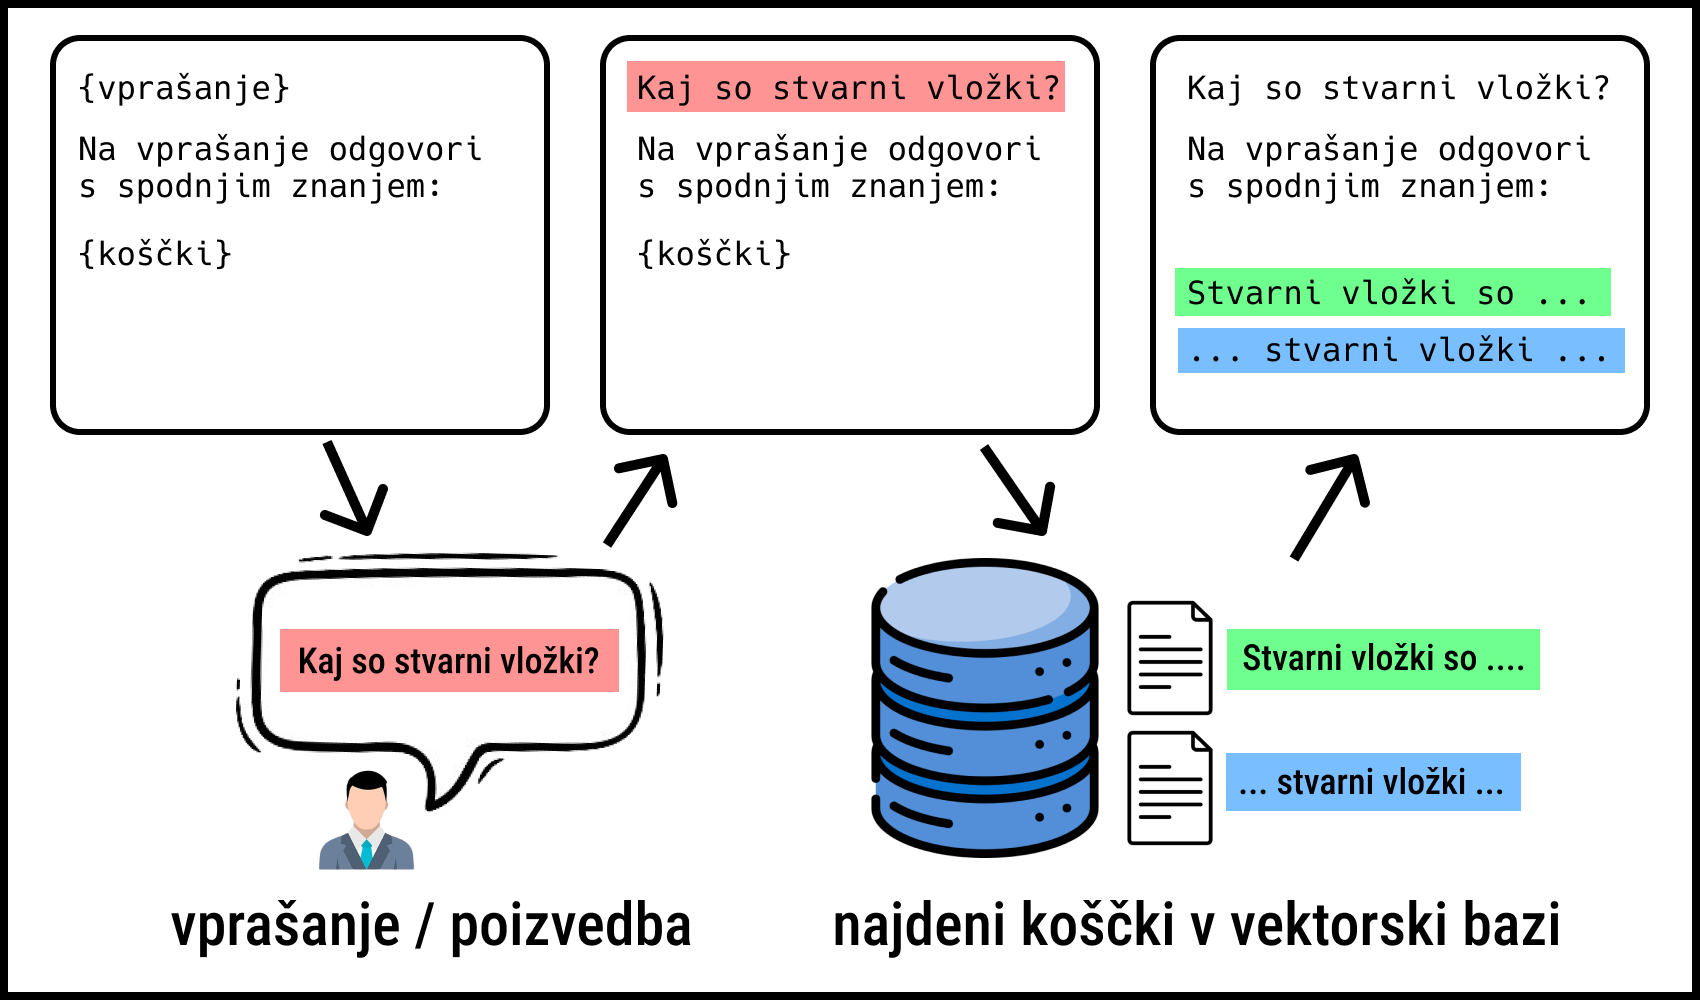
\includegraphics[width=\textwidth]{template.png}
	\caption{Postopek sestave vhoda za VJM pri tehnikah RAG}
	\label{template}
\end{figure}

Za hiter pregled zberemo na enem mestu še vse določene parametre:

\begin{itemize}
	\item \textbf{VJM}: Gemma 2. Se je izkazal za najprimernejši model za ta projekt.
	\item \textbf{Kodirnik}: Multiligual e5 large. Najuspešnejši majhen in večjezični kodirnik.
	\item \textbf{Dolžina koščkov}: 512 žetonov. Največje število žetonov, ki jih izbrani kodirnik sprejme na vhodu. Ker gre za naključno delitev, ni razloga, da bi delili na koščke krajše dolžine.
	\item \textbf{Vektorska baza}: Chroma. Učinkovita in praktična vektorska baza.
	\item \textbf{Število najdenih koščkov}: 5. Dovolj, a ne preveč konteksta in ne preseže maksimalnega števila žetonov VJM-ja.
\end{itemize}

\section{VJM + napredni RAG}

Zakon zdaj v primerjavi s prejšnjim pristopom razčlenimo glede na strukturne enote – člene. Vsak člen nadalje rekurzivno razdelimo na manjše enote, kot so odstavki, točke in alineje. Vsako enoto posebej vložimo. Tako imamo večje in manjše enote, nekatere zelo specifične, nekatere bolj splošne – od vsebine celotnega člena do posamezne alineje. Ko iskalnik najde košček, pogleda, v kateri enoti je vsebovan (če je) in razširi vsebino, da vključuje vse informacije. Ta tehnika se imenuje small2big \cite{small2big}. Primer: če je kot košček najdena alineja, se za besedilo ne vzame le ta alineja, temveč besedilo celotnega odstavka, v katerem je ta alineja.

Preden se vsebine razširijo, se jih še prerazporedi. To zagotavlja, da je možna informacija dejansko ustrezna za odgovor na vprašanje, ne le vsebinsko podobna.

Za model za ponovno sortiranje (angl. reranker) uporabljamo model bge-reranker-v2-m3 \cite{bge-reranker-v2-m3_1} \cite{bge-reranker-v2-m3_2}. Podobno kot pri kodirniku smo iskali majhen in večjezični model. Ta model smo izbrali zaradi njegove uspešnosti – metrike poročajo, da je uspešnejši od konkurentov.

Še preden pa se izvede kakršnakoli poizvedba, se uporabnikovo vprašanje spremeni v ustreznejšo obliko. To naredi VJM z navodili, naj vprašanje zastavi na bolj jasen način in uporablja pravno terminologijo. Ta komponenta je bila v ChatLaw-ju dodatno naučena na več milijon ročno ustvarjenih primerih, kar omogoča veliko večjo učinkovitost. VJM, uporabljen v tej nalogi, ni dodatno natreniran. Tako kot v vseh preostalih primerih je za VJM tu uporabljena Gemma 2 z naslednjimi navodili:

\begin{verbatim}
# Navodilo
Pretvori besedilo spodaj v pravni jezik, primeren 
za iskanje po pravnih dokumentih (zakonih).

Osredotoči se, da iz besedila vzameš vse pomembne informacije
in jih pretvoriš v pravno terminologijo.
Pravni dokumenti so napisani v pravni terminologiji.
Dokumente iščemo s primerjanjem semantičnosti besedil
(tj. rag vectorstore retrieval).
V ta namen želimo spodnje besedilo pretvoriti v ustrezno pravno obliko,
da najdemo vsebine, ki so najprimernejše za uporabnikovo poizvedbo. 

Pretvorba naj bo v preprosti tekstovni obliki,
brez kakršnegakoli formatiranja.

# Besedilo
{pretvorjena poizvedba}
\end{verbatim}

Zadnji del ostane enak kot pri naivnem RAG-u: najdeni koščki se v vrstnem redu podajo VJM-ju skupaj s prvotnim vprašanjem in navodilom, naj na vprašanje odgovori samo s podatki iz konteksta.

Še tu naredimo pregled določenih parametrov:

\begin{itemize}
	\item \textbf{VJM}: Gemma 2.
	\item \textbf{Kodirnik}: Multiligual e5 large.
	\item \textbf{Vektorska baza}: Chroma.
	\item \textbf{Število najdenih koščkov}: 50. Veliko število, saj jih pred generiranjem še ponovno sortiramo in tako morda najdemo kakšen prikrit, a pomemben košček. Več kot 50 je časovno prepotratno.
	\item \textbf{model za ponovno sortiranje}: BGE reranker v2 m3.
\end{itemize}

\section{VJM + modularni RAG}
\label{llm_kg_rag}

V predprocesiranju zakona zdaj izluščimo še reference in jih shranimo v grafno bazo. Torej za vsako omembo drugega dela zakona, ki se pojavi v besedilu, kot je npr. “... če je to v skladu s prvim odstavkom 42. člena tega zakona”, v grafni bazi shranimo povezavo med tema dvema entitetama.

Za grafno bazo uporabljamo Neo4j \cite{neo4j}. Izbira te grafne baze nima vpliva na uspešnost metod, saj je njena edina vloga shranjevanje (in vračanje) podatkov. Izbrali smo jo zaradi njene velike razširjenosti in pogostosti uporabe.

Vsega skupaj je 4.278 vozlišč, pridobljenih iz Zakona o gospodarskih družbah (testna množica). Vsako vozlišče je označeno kot dokument (ta je en sam), poglavje (strukturna enota, vključuje poglavja, odseke, pododseke itd.) ali element (vsebina zakonov). Vozlišča tvorijo drevesno strukturo z dokumentom v korenini vse do najmanjših elementov, kot so alineje prek poglavij, če upoštevamo le strukturne povezave. Strukturna povezava kaže od vozlišča do starša tega vozlišča.

Drug tip povezave v grafu so referenčne povezave. Za vsako omembo drugega dela zakona, ki se pojavi v kakšnem besedilu elementa, vzpostavimo povezavo med tema dvema vozliščema.

Postopek pridobivanja konteksta je enak kot pri naprednem RAG-u, le da imamo na koncu še en dodaten korak: Za vsak košček, ki ga damo VJM-ju, najprej združimo vse reference, ki so omenjene v besedilu koščka (s tem razširimo besedilo na vse informacije), ter vse reference, ki referencirajo ta košček in ga na kakršenkoli način spreminjajo.

S tem podamo VJM-ju vse potrebne informacije. Pri naprednem RAG-u za zgornji primer ne moremo vedeti, kaj so pogoji prvega odstavka 42. člena (ker le-ta ni bil najden ob poizvedbi), zaradi česar je odgovor pomanjkljiv, če ne celo napačen.

Parametri so identični kot pri naprednem RAG-u. Zraven sodi le še izbira grafne baze, ki je Neo4j.

Za vizualno primerjavo teh 4 metod si oglejte sliko \ref{rag_comparison}.

\begin{figure}[htbp]
	\centering
	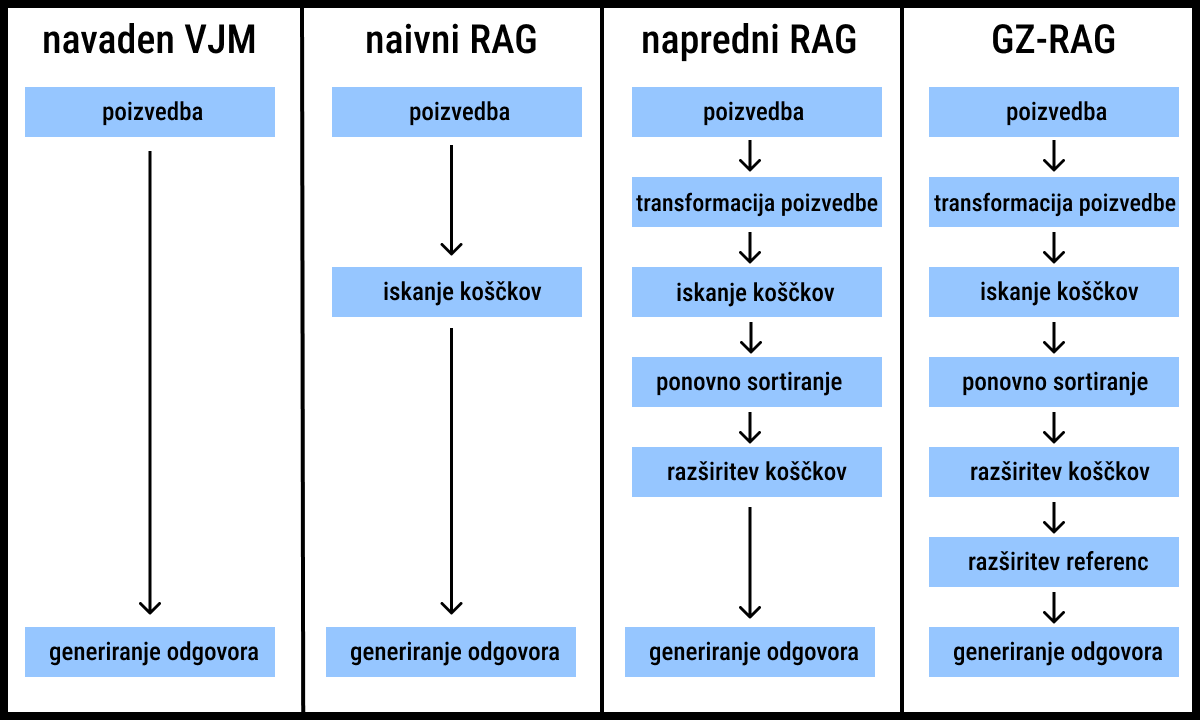
\includegraphics[width=\textwidth]{rag_comparison.png}
	\caption{Primerjava sestavnih delov implementiranih metod v tem delu.}
	\label{rag_comparison}
\end{figure}

\chapter{Vrednotenje in diskusija}
\label{ch4}

Vse 4 različne metode, opisane v poglavju Implementacija, smo testirali na 4 različnih scenarijih, opisanih v poglavju Podatki. Za testiranje smo uporabili testne primere, ki smo jih pripravili specifično za to raziskovalno delo.

\section{Kriteriji uspešnosti}

Uspešnost metod smo preverili na več načinov. V nadaljevanju so našteti uporabljeni kriteriji uspešnosti z njihovim opisom in namenom uporabe:

\begin{itemize}
	\item \textbf{BLEU}: preverja število ujemajočih se N-gramov med želenim in generiranim besedilom. Tipično se ta kriterij uspešnosti uporablja v prevajanju, tj. kako dobro računalniški sistem prevede besedilo v primerjavi s človekom. Za N se uporabijo različne vrednosti, nakar se te vrednosti še spremenijo s faktorji, ki penalizirajo pogosto uporabljene N-grame in prekratke prevode, da se doseže večja natančnost. Vrednosti se gibljejo med 0 in 1, kjer 0 pomeni, da med besediloma ni nobenega ujemanja, 1 pa predstavlja popolno ujemanje. Za primer te diplomske naloge ta kriterij uspešnosti preverja, ali se v generiranem odgovoru ključne besede pojavijo v določenem vrstnem redu (v lokalnem merilu). Velika pomanjkljivost je seveda ta, da se ne preverja semantičnost odgovora. Zato četudi VJM pravilno odgovori na vprašanje, vendar z drugačnimi besedami, bo dobil slabo oceno.
	\item \textbf{ROUGE-1}: se večinoma uporablja pri preverjanju kakovosti prevedenih besedil. Tako kot BLEU za gradnik primerjave vzame N-gram, pri ROUGE-1 je to 1-gram (besede). Ta kriterij uspešnosti preverja, če se pojavijo ključne besede v generiranem odgovoru in v kolikšnem številu. Tako kot pri BLEU je razpon od 0 do 1, kjer je 1 popolno ujemanje in 0 popolno neujemanje. Pomanjkljivosti so enake kot pri kriteriju BLEU.
	\item \textbf{ROUGE-L}: meri najdaljši (nepovezan) niz besed med generiranim in testnim besedilom. Tu je veliko bolj pomembno, v kakšnem vrstnem redu se pojavijo besede, v primerjavi z zgornjima dvema primeroma. Prav tako ni omejen na dejstvo, da se morajo besede vrstiti neposredno druga za drugo, vendar se lahko pojavijo v različnih (kasnejših) delih besedila. To nam omogoča, da bolje preverimo tekočnost odgovora, vendar še vedno ne zagotovi semantičnosti. Če se VJM namreč izrazi z drugačnimi besedami, kot so v testnem primeru, bo rezultat slab. Vendar v pravu je dosti domenske terminologije, kar bi moralo to težavo nekoliko uravnovesiti.
	\item \textbf{Človeška ocena (splošno)}: je daleč najpomembnejši kriterij uspešnosti, saj nam da vedeti, kako bi odgovore ocenil strokovnjak. Veliko bolj smo lahko prepričani, kako natančni in uporabni so odgovori dejansko v praksi. Prva različica človeške ocene preverja pravilnost odgovora v bolj splošnem pomenu, medtem ko ga spodnja različica preverja le v okviru predelane zakonodaje, tj. ZGD. Na primer vprašanje “Kaj so obveznosti revizijske komisije?” se da odgovoriti zunaj okvirja ZGD. Z znanjem, ki ga je JVM morda videl v drugih virih ali drugih oblikah med treniranjem.
	\item \textbf{Človeška ocena (ZGD)}: v primerjavi s splošno oceno v prejšnjem primeru se tu odgovor oceni izključno v okvirih ZGD. Revizijska komisija ima po ZGD neko definicijo in nanjo vezane določbe, ki se lahko razlikujejo od splošne prispodobe revizijske komisije in so bolj specifične. Z ločevanjem teh dveh primerov lahko razločimo, kako uspešno metode odgovarjajo v splošnem in v ozkem pogledu določenih besedil. Obe človeški oceni imata celo decimalsko oceno med 0 in 1 (odgovori so bili ocenjeni od 0 do 10 in kasneje deljeni z 10, da imajo ocene enak razpon kot prejšnji kriteriji).
\end{itemize}

\section{Rezultati}

Zaradi boljše preglednosti v tabelah rezultatov za metode uporabljamo naslednje oznake:

\begin{itemize}
	\item VJM: je prva metoda, tj. navadni VJM.
	\item RAG: je naivni RAG.
	\item n. RAG: je napredni RAG.
	\item GZ-RAG: pomeni graf znanje RAG. Gre za zadnjo metodo, modularni RAG oz. napredni RAG z grafno bazo.
\end{itemize}

Na začetku vsakega scenarija je tabela z rezultati. Tabeli sledita analiza in interpretacija rezultatov. Na koncu vsakega scenarija sta na voljo še dva primera generiranih odgovorov, en dober in en slab. Zaradi dolžine generiranih odgovorov za vsak scenarij v tem razdelku podamo le dva primera, da bralec dobi občutek za generirane odgovore. Več primerov si je možno ogledati v \hyperref[appendix_b]{Dodatku B}.

Vrednosti v tabelah predstavljajo povprečje rezultatov. Tako na primer vrednost 0,07 v tabeli \ref{rez1} za kriterij uspešnosti ROUGE-L pri metodi RAG pomeni, da je povprečna uspešnost te metode pri tem kriteriju za vseh deset vprašanj prvega scenarija enaka 0,07.

\subsection{Specifična vprašanja}

\begin{table}[H]
	\centering
	\caption{Ocene za specifična vprašanja.}
	\begin{tabular}{|l|c|c|c|c|}
		\hline
		kriterij uspešnosti    & VJM  & RAG  & n. RAG        & GZ-RAG        \\ \hline
		BLEU                   & 0,00 & 0,00 & \textbf{0,16} & 0,13          \\ \hline
		ROUGE-1                & 0,13 & 0,10 & 0,35          & \textbf{0,41} \\ \hline
		ROUGE-L                & 0,08 & 0,07 & 0,32          & \textbf{0,35} \\ \hline
		človeška ocena splošno & 0,46 & 0,25 & 0,62          & \textbf{0,76} \\ \hline
		človeška ocena ZGD     & 0,16 & 0,04 & 0,62          & \textbf{0,76} \\ \hline
	\end{tabular}
	\label{rez1}
\end{table}

Oglejmo si rezultate prvega scenarija v tabeli \ref{rez1}. Prva opazka je, da sta prvi dve metodi, navadni VJM in naivni RAG, občutno manj uspešni v primerjavi z naprednim in modularnim RAG-om. Vsi drugi kriteriji uspešnosti, razen kriterij splošne človeške ocene, nakazujejo na nezmogljivost teh dveh pristopov, da uspešno odgovorita na poizvedbe. Da splošna človeška ocena ni tako slaba, namiguje dejstvo, da so modeli sorodne koncepte videli v drugih situacijah (zunaj okvira ZGD) in jim je uspelo nekoliko bolje odgovoriti.

Da je navadni VJM uspešnejši od naivnega RAG-a si razlagamo tako, da s tem, ko modelu v naivnem RAG-u ukažemo, naj odgovori na vprašanje z najdenim znanjem, vendar se s podanimi podatki ne da odgovoriti na vprašanje (najdene vsebine se ne navezujejo na vprašanje), poskuša odgovoriti na vprašanje z napačnimi podatki, zaradi česar je odgovor napačen. Ker je že napredni RAG toliko bolj uspešen od naivnega RAG-a, potrdi hipotezo, da je izbira velikosti koščkov pri pred procesiranju podatkov zelo pomembna, saj nam omogoči, da bolj natančno najdemo pravilno vsebino

Nekoliko zanimivo je videti, da je GZ-RAG uspešnejši od naprednega RAG-a. V tem scenariju tega nismo pričakovali, saj glede na to, da so vse potrebne informacije za pravilen odgovor dostopne na enem mestu (in je treba ta košček le pravilno najti), nam besedilo iz referenc ne bi kaj dosti pomagalo.

Da sta obe človeški oceni enaki pri naprednem RAG-u in GZ-RAG-u pomeni, da sta modela odgovarjala ekskluzivno z najdeno literaturo, tj. najdenim znanjem iz ZGD, in da se splošni in kontekst ZGD nista razlikovala.

Druga opazka je ta, da avtomatskima kriterijema uspešnosti, BLEU in ROUGE, ne uspe efektivno oceniti uspešnosti odgovorov. Recimo pri navadnem VJM-ju sta BLEU in ROUGE kriterija uspešnosti blizu 0, medtem ko je splošna človeška ocena nekoliko pod 0.5. N-grami in prekrivanja besedila, kot kaže nista zadostni merili za preverjanje semantične pravilnosti odgovora.

Odločitev manjšega števila testnih primerov in posledično možnost ročnega ocenjevanja se je izkazala kot dobra odločitev, saj bi v nasprotnem primeru narobe interpretirali rezultate glede na druge kriterije.

\underline{\textbf{Primera generiranih odgovorov.}}

\textbf{Vprašanje: Na kaj je treba biti pozoren pri vrednotenju sredstev in obveznosti do vira sredstev, ki na podlagi združitve ali delitve preidejo na prevzemno družbo?}

\textit{Naiven RAG, človeška ocena splošno: 0, človeška ocena ZGD: 0}

\textit{Komentar: Odgovor je popolnoma napačen.}

\begin{mdframed}[linewidth=1pt]
	\raggedright
	\ttfamily
	Poročilo revizijskega pregleda je pomemben dokument, ki pomaga organizaciji pri izboljšanju svojega poslovanja in upravljanja. Revizijski komisiji omogoča informiran sprejem odločitev glede finančnega stanja, notranje kontrole in varnosti sredstev organizacije.

	Pri vrednotenju sredstev in obveznosti do vira sredstev, ki na podlagi združitve ali delitve preidejo na prevzemno družbo, je treba biti pozoren na naslednje:

	**Sredstva:**

	* **Vrednotenje po izvirni ceni:** V kolikor so sredstva že bilene v obstoječih knjigah, se mora njihova vrednost prilagoditi novi družbi. To pomeni, da je treba upoštevati morebitne razlike v računovodskih politikah in standardih med združenimi družbami. \\
	* **Vrednotenje po tržni ceni:** V primeru nematerialnih sredstev (npr. blagovne znamke, patentski pravice) je treba upoštevati njihovo tržno vrednost. \\
	* **Prihodki in izgubi:** Pri prenosu poslovnih aktivnosti na prevzemno družbo je treba upoštevati morebitne prihodke in izgube, ki nastanejo v času prenosa.

	**Obveznosti:**

	* **Vrednotenje po nominalni vrednosti:** Obveznosti se običajno vrednotijo po nominalni vrednosti, ki je navedena v pogodbah. \\
	* **Prilagoditev za inflacijo:** V kolikor so obveznosti dolgoveče, je treba upoštevati morebitne prilagoditve zaradi inflacije. \\
	* **Nedoločene obveznosti:** Je treba preveriti, ali obstajajo neomejene obveznosti, ki jih ni mogoče izrecno ugotoviti v pogodbah, in jih primerno vrednotiti.

	**Viri sredstev:**

	* **Prehod kapitala:** Pri združitvi družb se kapital prenese na prevzemno družbo. V kolikor gre za delitvijo družbe, se kapital razdeli med ustanovljene družbe. \\
	* **Prevod rezerv in prihrankov:** Rezervne sklade in prihranki se običajno preselijo na prevzemno družbo.

	**Ostalo:**

	* **Poslovni model:** Vrednotenje sredstev in obveznosti je treba izvesti v okviru poslovnega modela prevzemne družbe, kar pomeni, da je treba upoštevati morebitne spremembe v strategiji in operativnih procesih. \\
	* **Nejasnosti in tveganja:** Vrednotenje prehodnih sredstev in obveznosti je lahko zapleteno in zahteva temeljito analizo. Je treba pozornost nameniti morebitnim nejasnostim in tveganjem, ki se pojavijo v času združitve ali delitve družb.

	Pri vrednotenju prehodnih sredstev in obveznosti je priporočljivo, da se izvede neodvisna revizija s strani certificiranega računovodskega podjetja.
\end{mdframed}

\textit{Napreden RAG, človeška ocena splošno: 10, človeška ocena ZGD: 10}

\textit{Komentar: Odgovor je jedrnat in vključuje vse potrebne informacije.}

\begin{mdframed}[linewidth=1pt]
	\raggedright
	\ttfamily
	Po podatkih, ki ste jih zagotovili, morajo biti sredstva in obveznosti do virov sredstev, ki na podlagi združitve ali delitve preidejo na prevzemno družbo, **ovrednoteni v skladu s slovenskimi računovodskimi standardi ali mednarodnimi standardi računovodskega poročanja**.
\end{mdframed}

\subsection{Specifična vprašanja z referencami}

\begin{table}[H]
	\centering
	\caption{Ocene za specifična vprašanja z referencami.}
	\begin{tabular}{|l|c|c|c|c|}
		\hline
		kriterij uspešnosti    & VJM  & RAG  & n. RAG & GZ-RAG        \\ \hline
		BLEU                   & 0,02 & 0,01 & 0,12   & \textbf{0,17} \\ \hline
		ROUGE-1                & 0,22 & 0,22 & 0,45   & \textbf{0,46} \\ \hline
		ROUGE-L                & 0,14 & 0,13 & 0,38   & \textbf{0,38} \\ \hline
		človeška ocena splošno & 0,36 & 0,38 & 0,58   & \textbf{0,81} \\ \hline
		človeška ocena ZGD     & 0,07 & 0,07 & 0,59   & \textbf{0,81} \\ \hline
	\end{tabular}
	\label{rez2}
\end{table}

V tabeli \ref{rez2} podobno vidimo rezultate kot v prejšnjem testnem scenariju (\hyperref[rez1]{Tabela 5.1}). Prvi dve metodi sta dokaj manj uspešni od zadnjih dveh. ROUGE-1 je višja pri vseh metodah, kar pomeni, da so modeli v tem scenariju uporabljali več ključnih besed oz. besed, ki se pojavijo v pravilnem odgovoru.

Človeška ocena za prvi dve metodi je podobna kot prej: splošno sta nekoliko uspešni, kar nakazuje na osnovno splošno razumevanje koncepta, vendar ne v okviru ZGD.

GZ-RAG je odločno najuspešnejši. Dodatne informacije, ki jih VJM dobi prek referenc, naredijo veliko razliko, s tem da modelu podajo več potrebnih informacij za pravilen odgovor. To je pomanjkljivost, ki se vidi v naprednem RAG-u. Medtem ko je v prejšnjem scenariju dohajal GZ-RAG in referencirani koščki niso med najdenimi, zaradi česar odgovor ni nujno napačen, le pomanjkljiv.

\underline{\textbf{Primera generiranih odgovorov.}}

\textbf{Vprašanje: Katere družbe morajo sestaviti računovodsko poročilo v skladu z mednarodnimi standardi računovodskega poročanja?}

\textit{Navaden VJM, človeška ocena splošno: 6, človeška ocena ZGD: 5}

\textit{Komentar: ZGD-1 ne pozna trgovskih družb, ampak govori o delniških družbah, ki so subjekti javnega interesa. Pri ostalih, ki se prostovoljno odločijo, pa niso podani dodatni pogoji, ki jih ZGD-1 določa.}

\begin{mdframed}[linewidth=1pt]
	\raggedright
	\ttfamily
	Vse javno trgovske družbe (tj. tiste, ki prodajajo svoje delnice na borzi) so dolžan obvestiti o svoji finančni situaciji s sestavo in objavo računovodskega poročila v skladu z mednarodnimi standardi računovodskega poročanja (IFRS).

	Poleg tega morajo nekatera podjetja, ki niso javno trgovske družbe, vendar sodelujejo na finančnih trgih ali imajo določene oblike lastništva, sestaviti računovodska poročila v skladu z IFRS. To lahko vključuje:

	* **Družbe, ki se odločijo za uporabo IFRS,** čeprav niso dolžane. \\
	* **Holding družbe**

	Zahteve za pripravo računovodskega poročila v skladu z IFRS se lahko razlikujejo glede na državo in zakonodajo.


	Za natančnejšo informacije o tem, katerih družb je obvezno sestaviti računovodska poročila v skladu z IFRS, vam priporočam, da se posvetlite pri izbranem računovoditelju ali pravnem svetovalcu.

\end{mdframed}

\textit{Modularen RAG, človeška ocena splošno: 8, človeška ocena ZGD: 8}

\textit{Komentar: Metoda ni navedla kaj pravi ta člen zakona in manjka, da po MSRP sestavljajo še tiste, s katerimi vrednostnimi papirji se trguje na organiziranih trgih.}

\begin{mdframed}[linewidth=1pt]
	\raggedright
	\ttfamily
	Na podlagi navedenih podatkov morajo naslednje družbe sestaviti računovodsko poročilo v skladu z mednarodnimi standardi računovodskega poročanja:

	* **Družbe iz enajstega odstavka 54. člena tega zakona:**  prvič to počnete za poslovno leto, ki se začne leta 2006. \\
	* **Banke:** prvič to počnete za poslovno leto, ki se začne leta 2006. \\
	* **Zavarovalnice:** prvič to počnete za poslovno leto, ki se začne leta 2007.

	Pomembno je omeniti, da veljajo določbe tega poglavja tudi za kapitalske družbe in tiste osebne družbe, pri katerih za njihove obveznosti ni neomejeno odgovorna nobena fizična oseba.

\end{mdframed}

\subsection{Splošna vprašanja}

\begin{table}[H]
	\centering
	\caption{Ocene za splošna vprašanja.}
	\begin{tabular}{|l|c|c|c|c|}
		\hline
		kriterij uspešnosti    & VJM  & RAG  & n. RAG        & GZ-RAG        \\ \hline
		BLEU                   & 0,00 & 0,00 & 0,03          & \textbf{0,04} \\ \hline
		ROUGE-1                & 0,25 & 0,25 & 0,30          & \textbf{0,30} \\ \hline
		ROUGE-L                & 0,13 & 0,12 & \textbf{0,21} & 0,18          \\ \hline
		človeška ocena splošno & 0,22 & 0,18 & \textbf{0,58} & 0,54          \\ \hline
		človeška ocena ZGD     & 0,07 & 0,02 & \textbf{0,58} & 0,53          \\ \hline
	\end{tabular}
	\label{rez3}
\end{table}

Napredni RAG je v tem scenariju (rezultati so vidni v tabeli \ref{rez3}) uspešnejši kot GZ-RAG. Razlike so majhne (predvsem na tako majhni testni množici niso tako statistično pomembne), tako da ne moremo z gotovostjo trditi, kaj je odločilni faktor, vendar si lahko razlagamo sledeče: v tem scenariju se preverja, ali so najdene vse ustrezne vsebine, ki so v več različnih členih. Zatorej ni tako pomembno, da za najdene člene vključimo njihove reference, marveč dejstvo, da jih sploh najdemo. Torej se je v naprednem RAG-u našlo več ustreznih členov, s katerimi je bilo mogoče odgovoriti na vprašanja. Dodatno razširjeno besedilo, pridobljeno prek referenc, pa ni niti približno prineslo take teže kot v prejšnjem scenariju.

Dodatna razlaga je možnost predolgega konteksta v primeru GZ-RAG-a. Za vsakega od najdenih koščkov namreč povlečemo še vso referencirano besedilo, kar v nekaterih primerih lahko pomeni vsebino celotnih členov, in je vhod v VJM mnogo daljši kot pri naprednem RAG-u. To predstavlja dve težavi: prvič, informacij je veliko več in presoditi, katere so pomembne, ima več možnosti za napako; drugič, če je skupek dolžine vseh besedil predolg in preseže maksimalno dolžino vhoda VJM-ja, se besedilo grobo odseka pri maksimalnem številu žetonov. Tako se del znanja (najdenih koščkov) sploh ne pojavi v vhodu VJM-ja.

Opazi se tudi manjša uspešnost naprednega RAG-a in GZ-RAG-a, vsaj glede na človeške ocene. Oba kriterija ROUGE sta višja kot v prejšnjih dveh scenarijih, kar nakazuje na to, da so generirani odgovori bolj skladni s pravilnimi iz testne množice.

Navadni VJM in naivni RAG tu prav tako ne izkazujeta dobrih rezultatov.

\underline{\textbf{Primera generiranih odgovorov.}}

\textbf{Vprašanje: Do kdaj in komu mora družba oddati letno poročilo?}

\textit{Naiven RAG, človeška ocena splošno: 2, človeška ocena ZGD: 0}

\textit{Komentar: AJPES ni agencija za javne usluge, napačno navaja, da se oddaja do konca junija – eden rok je konec marca, drugi konec avgusta glede na zahteve zakonodaje.}

\begin{mdframed}[linewidth=1pt]
	\raggedright
	\ttfamily
	V Sloveniji morajo družbe letno poročilo oddati **AJPES (Agenciji za javne usluge)**.

	Obveznost za izdajanje letnega poročila velja za vse družbe, ki niso v skladu z določbami Zakona o preprečevanju pranja denarja in financiranja terorizma (ZPPDFT).

	Letno poročilo mora biti oddano **do konca junija** v letu po poslovnem letu.

	Poleg AJPES, letno poročilo lahko družba objavi tudi na svoji spletni strani ali ga razdeli drugim zainteresiranim strankam, kot so investitorji in dobavitelji.
\end{mdframed}

\textit{Napreden RAG, človeška ocena splošno: 8, človeška ocena ZGD: 8}

\textit{Komentar: Dva roka sta glede na velikost družbe in zavezanost reviziji – spustil je rok, ki velja za manjhne družbe, ki niso zavezane reviziji. Rok je konec marca.}

\begin{mdframed}[linewidth=1pt]
	\raggedright
	\ttfamily
	Družba mora letno poročilo skupaj z revizorjevim poročilom oddati **Agenciji Republike Slovenije za javnopravne evidence in storitve (AJPES)** v **osmih mesecih po koncu poslovnega leta**.


	V primeru, da gre za družbe iz prvega odstavka 53. člena tega zakona, morajo poleg letnega poročila še predložiti **predlog razporeditve dobička ali obravnavanja izgube ter razporeditev dobička ali obravnavanje izgube**.
\end{mdframed}

\subsection{Konkretni primeri}

\begin{table}[H]
	\centering
	\caption{Ocene za konkretne primere.}
	\begin{tabular}{|l|c|c|c|c|}
		\hline
		kriterij uspešnosti    & VJM  & RAG  & n. RAG        & GZ-RAG        \\ \hline
		BLEU                   & 0,00 & 0,00 & 0,05          & \textbf{0,05} \\ \hline
		ROUGE-1                & 0,22 & 0,21 & 0,31          & \textbf{0,32} \\ \hline
		ROUGE-L                & 0,11 & 0,11 & \textbf{0,21} & 0,18          \\ \hline
		človeška ocena splošno & 0,11 & 0,15 & \textbf{0,71} & 0,69          \\ \hline
		človeška ocena ZGD     & 0,00 & 0,00 & \textbf{0,73} & 0,66          \\ \hline
	\end{tabular}
	\label{rez4}
\end{table}

Interpretirajmo še rezultate četrtega scenarija, kjer so rezultati prikazaniv tabeli \ref{rez4}. Prva opazka so višje človeške ocene pri zadnjih dveh metodah v primerjavi s prejšnjim scenarijem. Pričakovali smo nižje. Vprašanja v prejšnjem scenariju so bila postavljena natančno in v ustrezni terminologiji, medtem ko so v tem scenariju ista vprašanja, posplošena v njihovo bolj poljudno obliko. Transformerji poizvedbe so naredili odlično delo, da je modelom uspelo najti ustrezne koščke, napisane v pravni terminologiji. Vendar ne smemo zanemariti dejstva, da tako kot vprašanja so tudi odgovori podani v bolj poljudni obliki. Znano dejstvo je, da so VJM-ji bolj uspešni na splošnih področjih ter vse manj uspešni in natančni na vse bolj domenskem znanju. Torej so bili generirani odgovori v tem scenariju primernejši kot v prejšnjem, saj so VJM-ji uspešnejši v poljudnem okolju.

\underline{\textbf{Primera generiranih odgovorov.}}

\textbf{Vprašanje: Kdaj za namene letnega poročanja poročamo kot velika družba?}

\textit{Navaden VJM, človeška ocena splošno: 0, človeška ocena ZGD: 0}

\textit{Komentar: Čisto narobe. Nimamo termina brutoprihodki, bilance katere, ne velja (in tudi nimamo) zakona o računovodstvu (je ZGD-1) in zakona o javnem računovodstvu (sploh ne obstaja).}

\begin{mdframed}[linewidth=1pt]
	\raggedright
	\ttfamily
	V Sloveniji velja, da podjetje poroča kot velika družba za namene letnega poročanja, če **vsaj tri od naslednjih meritev izpolnjuje**:

	* **Bruto prihodki:** vsaj 20 milijonov evrov \\
	* **Povprečna število zaposlenih:** vsaj 50 oseb v poslovnem letu \\
	* **Bilance:** vsaj 10 milijonov evrov

	To pomeni, da mora podjetje prikazati podatke o svoji dejavnosti po posebnih standardih (zakon o računovodstvu) in oblikovati letno poročilo v skladu z zahtevami Zakona o javnem računovodstvu.


	POMEMBNO: Vprašanje je precej strokovno in odgovor se nanaša na splošno veljavna pravila v Sloveniji. Za natančen odgovor glede vašega podjetja je potrebno posvetovanje s pravnikom ali davčnim svetovalcem.
\end{mdframed}

\textit{Modularen RAG, človeška ocena splošno: 9, človeška ocena ZGD: 9}

\textit{Komentar: Manjka da pogleda kdo je velika družba in navede kriterije.}

\begin{mdframed}[linewidth=1pt]
	\raggedright
	\ttfamily
	Za namene letnega poročanja poročate kot velika družba, če ste ena izmed naslednjih:

	* **banka** \\
	* **zavarovalnica** \\
	* **borza vrednostnih papirjev** \\
	* **družba, ki po 56. členu tega zakona mora pripraviti konsolidirano letno poročilo.**

	Vendar pazite! To se nanaša samo na letno poročanje. Obstajajo še različne klasifikacije družb glede na število zaposlenih, čisti prihodki in vrednost aktiv.
\end{mdframed}

\subsection{Primerjava naših metod s Pravkom}

Zdaj naredimo še primerjavo s Pravkom, da ocenimo, kako uspešne so naše metode v primerjavi z že obstoječimi rešitvami. Ker je za neplačniške uporabnike število vprašanj, ki jih lahko postavimo Pravku, omejeno na 5, smo tako za vsak scenarij Pravku postavili le eno vprašanje iz naše testne množice. S tem dobimo bolj informativno primerjavo, za konkretnejšo bi se bilo treba naročiti na Pravkove storitve in narediti bolj temeljito primerjavo. Za vprašanja smo izbrali tista, pri katerih so bile naše metode (dokaj) uspešne, vendar je še prostor za izboljšavo. Na ta način lahko bolje razločimo, kako je Pravko uspešen v primerjavi z našimi metodami.

\begin{table}[H]
	\centering
	\caption{Primerjava naših metod s Pravkom.}
	\begin{tabular}{|l|c|c|c|c|c|}
		\hline
		scenarij   & VJM  & RAG  & n. RAG        & GZ-RAG        & Pravko        \\ \hline
		scenarij 1 & 0,70 & 0,40 & 0,60          & \textbf{0,90} & 0,80          \\ \hline
		scenarij 2 & 0,40 & 0,40 & 0,80          & 0,80          & \textbf{0,90} \\ \hline
		scenarij 3 & 0,40 & 0,20 & \textbf{0,80} & \textbf{0,80} & 0,20          \\ \hline
		scenarij 4 & 0,30 & 0,30 & 0,70          & 0,80          & \textbf{0,90} \\ \hline
	\end{tabular}
\end{table}

Pravko ima uspešne rezultate, primerljive z naprednim in modularnim RAG-om. Razen tretjega scenarija, kjer ima Pravko slabši rezultat kot celo navadni VJM, so rezultati na isti ravni kot pri modularnem RAG-u. Naše metode, predvsem napredni in modularni RAG, so podobno uspešne kot Pravko.

Pomembno je omeniti, da smo za vsak scenarij preverili le eno vprašanje in to je bilo izbrano tako, da so naše metode uspešno odgovorile nanj. Da bi z gotovostjo lahko kaj trdili, bi bila potrebna bolj obsežna primerjava.

\section{Diskusija}

Navadni VJM in naivni RAG nikakor nista primerna za kakršnokoli uporabo. Od navadnega VJM-ja smo to tudi pričakovali, saj (zelo verjetno) slovenska zakonodaja in s tem ZGD ni bil v korpusu učnih podatkov, torej potrebnega znanja za pravilen odgovor nima. Po splošnih človeških ocenah vidimo, da do neke mere še ponudi uporabno informacijo, vendar premalokrat in premalo zanesljivo.

Od naivnega RAG-a smo pričakovali več, če ne drugega vsaj večjo uspešnost kot pri navadnem VJM-ju, ki je bil primerjalna točka. Da je uspešnost slabša, lahko pomeni le, da najdena besedila niso prav nič pripomogla k pravilnosti odgovora, če niso na mestih celo škodila. Očiten razlog so napačno najdena besedila, tj. besedila členov, ki smo jih dali VJM-ju, niso pomembna za vprašanje. Vprašanja so bila strokovno postavljena, zato pomanjkanje transformacije poizvedbe ne bi smelo biti težava. Ostaneta še velikost koščkov in prerazporejanje. Nagibamo se k mnenju, da je večji vpliv na slabo uspešnost imela velikost koščkov, kar je povzročilo, da najdeni koščki niso bili ustrezni za odgovor.

Največji preskok je med naivnim RAG-om in naprednim RAG-om. Če so podatki bolje pripravljeni in se jih lažje najde, so tudi odgovori bolj natančni. Če tega ni, so torej razlike v natančnosti odgovorov velike. Med naprednim in modularnim RAG-om so razlike dosti manjše, kar smo do določene mere tudi pričakovali. Medtem ko je med naivnim in naprednim RAG-om kopica izboljšav, se GZ-RAG od naprednega RAG-a razlikuje le v zadnjem koraku, ko za vsak košček zbere še vsa referencirana besedila. Ko je poudarek na tej lastnosti, kot je bil v scenariju 2, se vidi, da je GZ-RAG uspešnejši od naprednega RAG-a. V primerih, ko so vse (ali večina) informacij zbrane na enem mestu (člen), ni kaj nadgraditi. Ali če referencirane informacije ne prinesejo koristnih informacij, so lahko le motilec, zaradi česar naprednemu RAG-u ni treba razločevati med pomembnimi in nepomembnimi informacijami in je v teh primerih uspešnejši, kot je bil v scenarijih 3 in 4.

Kot smo že omenili, prvi dve metodi za pravnega asistenta nista primerni za uporabo. Kot kaže, je pravo še vedno posebno področje, ki potrebuje specializirane rešitve namesto generičnih. Zadnji dve metodi kažeta, da bi se z nadaljnjimi izboljšavami ti sistemi lahko začeli uporabljati v praksi. Ne še na ravni splošnega svetovalca, vendar mogoče kot pomočnik pravnemu delavcu, kjer je oseba v stalnem kontaktu z zakonodajo.

\chapter{Zaključek}
\label{ch5}

Cilj tega raziskovalnega dela je bilo odgovoriti na vprašanje, ali se pravni asistent (VJM) lahko uporablja v vsakodnevnih situacijah. Ker je pravo kompleksno področje, smo predstavili več različnih metod. Za največji problem se je izkazalo pomanjkanje pravnega znanja VJM-ja, predvsem kar se tiče Zakona o gospodarskih družbah, zaradi česar smo predlagali tehniko RAG, da bi VJM-ju umetno podali potrebno znanje.

Rezultati nakazujejo, da je še veliko prostora za izboljšavo metod. Navadni VJM in naivni RAG nista uspešna v praktično nobenem primeru, njuni rezultati so zelo slabi v vseh preizkušenih scenarijih. Napredni RAG in GZ-RAG dosežeta primerljivo uspešnost, ki je približno na enaki ravni. Največja razlika med njima se je pokazala v drugem scenariju, kjer je bilo referencirano besedilo ključno za odgovor.

V prvih dveh scenarijih sta se tako napredni RAG kot GZ-RAG izkazala za močna kandidata. Uspešnost je bila zadostna, da bi se z nekaj nadaljnjimi popravki te metode že lahko začele uporabljati v praksi, z GZ-RAG-om v ospredju. Za splošnejša vprašanja je prihodnost nekoliko bolj meglena. Rezultati še niso na zadostni ravni, da bi se te metode lahko zanesljivo uporabljale v kritičnih sistemih.

Za nadaljnje raziskovanje bi bilo smiselno dotrenirati VJM na slovenski zakonodaji. S tem bi omogočili veliko boljše razumevanje vprašanj z domenskega vidika, poznavanje terminologije in interno znanje zakonov. Tedaj bi tudi pri uporabi RAG-a VJM lahko bolj natančno ubesedil in izrazil odgovor (strokovnjak se bo izrazil bolj strokovno dosledno kot povprečen človek). Pretvorba poizvedbe iz vsakodnevnega jezika v pravno terminologijo bi bila na ta način močno izboljšana.

Naslednja očitna izboljšava je razširitev korpusa. Vključiti bi bilo treba več pravnih aktov, med njimi vzpostaviti povezave in preveriti, kako se metode vedejo v primeru te večje množice. Nazadnje bi bilo mogoče raziskati, kako se izboljša učinkovitost, če vpeljemo več specializiranih in avtonomnih enot v proces, podobno, kot je to v projektu ChatLaw.

Kot nakazuje dejstvo, da sta Pravko in ChatLaw javno dostopna in na voljo za uporabo, potreba po pravnih asistentih obstaja. Tako kot vsaka nova tehnologija bo tudi to področje z nadaljnjim raziskovanjem postalo naše vsakodnevno orodje, s katerim lahko izboljšamo naše življenje.


\cleardoublepage
%\addcontentsline{toc}{chapter}{Literatura}

% če imaš težave poravnati desni rob bibliografije, potem odkomentiraj spodnjo vrstico
\raggedright

% \printbibliography[heading=bibintoc,type=article,title={Članki v revijah}]

% \printbibliography[heading=bibintoc,type=inproceedings,title={Članki v zbornikih}]

% \printbibliography[heading=bibintoc,type=incollection,title={Poglavja v knjigah}]

% v zadnji verziji diplomskega dela običajno združiš vse tri vrste referenc v en sam seznam in
% izpustiš delne sezname
\printbibliography[heading=bibintoc,title={Literatura}]

\cleardoublepage

\phantomsection
\addcontentsline{toc}{chapter}{Dodatek A: Vprašanja v\\testni množici}
\chapter*{Dodatek A: Vprašanja v testni množici}
\label{appendix_a}

V tem dodatku si lahko ogledate vsa vprašanja za vsakega od testnih scenarijev. Vprašanju sledi tudi pravilen odgovor. Vprašanja so postavljena v odebeljenem tisku.

\section*{Scenarij 1: specifična vprašanja}

\textbf{Kako pogosto je potrebno preveriti, ali se stanje posameznih aktivnih in pasivnih postavk v poslovnih knjigah ujema z dejanskim stanjem?}

Najmanj enkrat letno

\textbf{Kaj je mikro družba?}

Mikro družba je družba, ki izpolnjuje dve od teh meril:
- povprečno število delavcev v poslovnem letu ne presega deset,
- čisti prihodki od prodaje ne presegajo 2.000.000 eurov, in
- vrednost aktive ne presega 2.000.000 eurov.

\textbf{O čem mora revizor poročati revizijski komisiji?}

Revizor mora revizijsko komisijo obveščati o glavnih zadevah v zvezi z revizijo letnega poročila, zlasti o pomembnih pomanjkljivostih notranjih kontrol v povezavi s postopkom računovodskega poročanja.

\textbf{Na kaj je treba biti pozoren pri vrednotenju sredstev in obveznosti do vira sredstev, ki na podlagi združitve ali delitve preidejo na prevzemno družbo?}

Da se morajo ovrednotiti v skladu s slovenskimi računovodskimi standardi ali mednarodnimi standardi računovodskega poročanja.

\textbf{Kaj se zgodi s podjetjem, če podjetnik umre?}

Če podjetnik umre, lahko podjetnikov dedič, ki nadaljuje zapustnikovo podjetje, v firmi še naprej uporablja tudi ime in priimek zapustnika. Z nadaljevanjem zapustnikovega podjetja preidejo na podjetnikovega dediča podjetje podjetnika ter pravice in obveznosti podjetnika v zvezi s podjetjem. Podjetnikov dedič kot univerzalni pravni naslednik vstopi v vsa pravna razmerja v zvezi s prenesenim podjetjem podjetnika .

\textbf{Kaj vsebuje firma podjetnika?}

Firma podjetnika vsebuje ime in priimek podjetnika, skrajšano oznako, da gre za samostojnega podjetnika (s.p.), oznako dejavnosti in morebitne dodatne sestavine.

\textbf{Ali prokura preneha s smrtjo ali izgubo poslovne sposobnosti podjetnika?}

Ne.

\textbf{Kdaj lahko podjetnik poslovne knjige void po sistemu enostavnega knjigovodstva?}

Podjetnik vodi poslovne knjige po sistemu enostavnega knjigovodstva, če ni v zadnjem poslovnem letu prekoračil dveh od teh meril:
- da povprečno število delavcev ne presega tri,
- da so letni prihodki nižji od 50.000 eurov,
- da povprečna vrednost aktive, izračunana kot polovica seštevka vrednosti aktive na prvi in zadnji dan poslovnega leta, ne presega 25.000 eurov. To velja tudi za podjetnika, ki začne opravljati dejavnost in v prvem poslovnem letu ne zaposluje povprečno več kot tri delavce.

\textbf{Kateri premoženjski predmeti se ne štejejo kot stvarni vložki ali stvarni prevzem?}

Kot stvarni vložki ali stvarni prevzem se lahko štejejo le tisti premoženjski predmeti ali pravice, katerih gospodarska vrednost je ugotovljiva. Dolžnost opraviti storitev se ne šteje za stvarni vložek ali stvarni prevzem v smislu tega člena.

\textbf{Kdaj za ustanovitev s stvarnimi vložki ni potrebno mnenje revizorja?}

Ustanovitvenemu revizorju ni treba pregledati ustanovitve:
- če so predmet stvarnega vložka prenosljivi vrednostni papirji ali instrumenti denarnega trga, kakor jih določa zakon, ki ureja trg finančnih instrumentov, in je njihova vrednost določena kot tehtano povprečje enotnega tečaja, doseženega na enem ali več organiziranih trgih, kakor jih določa zakon, ki ureja trg finančnih instrumentov, v najmanj šest mesečnem obdobju, ki se konča en teden pred dnevom sprejema statuta;
- če je predmet stvarnega vložka, razen prenosljivih vrednostnih papirjev in instrumentov denarnega trga iz prejšnje alineje, že bil vrednoten s strani revizorja največ šest mesecev pred dnevom izročitve predmeta stvarnega vložka in je bilo vrednotenje opravljeno v skladu s splošno priznanimi standardi in načeli vrednotenja, ali
- če izvira poštena vrednost predmeta stvarnega vložka, razen prenosljivih vrednostnih papirjev in instrumentov denarnega trga iz prve alineje 194a. člena ZGD-1, iz posameznega predmeta stvarnega vložka, izkazanega v revidiranem letnem poročilu prejšnjega poslovnega leta.

\section*{Scenarij 2: Specifična vprašanja z referencami}

\textbf{Kaj je majhna družba?}

Majhna družba je družba, ki izpolnjuje dve od teh meril:
- povprečno število delavcev v poslovnem letu ne presega 50,
- čisti prihodki od prodaje ne presegajo 8.800.000 eurov, in
- vrednost aktive ne presega 4.400.000 eurov.

Mikro družba je družba, ki izpolnjuje dve od teh meril:
- povprečno število delavcev v poslovnem letu ne presega deset,
- čisti prihodki od prodaje ne presegajo 2.000.000 eurov, in
- vrednost aktive ne presega 2.000.000 eurov.

\textbf{Kaj je velika družba?}

Velika družba je družba, ki ni srednja družba glede na naslednje kriterije:

Srednja družba je družba, ki ni mikro družba ali majhna družba, in ki izpolnjuje dve od teh meril:
- povprečno število delavcev v poslovnem letu ne presega 250,
- čisti prihodki od prodaje ne presegajo 35.000.000 eurov, in
- vrednost aktive ne presega 17.500.000 eurov.

\textbf{Katere družbe morajo sestaviti računovodsko poročilo v skladu z mednarodnimi standardi računovodskega poročanja?}

Družbe, katerih vrednostni papirji so uvrščeni na katerega od organiziranih trgov vrednostnih papirjev v državah članicah Evropske skupnosti, morajo sestaviti konsolidirano letno poročilo v skladu z mednarodnimi standardi računovodskega poročanja.

Poleg družb iz prejšnjega odstavka sestavljajo računovodska poročila v skladu z mednarodnimi standardi računovodskega poročanja tudi:
1. banke,
2. zavarovalnice, in
3. druge družbe, če tako odloči skupščina družbe, vendar najmanj za pet let.

\textbf{Iz česa je sestavljeno letno poročilo družb?}

Letno poročilo družb je sestavljeno iz:
- bilance stanja,
- izkaza poslovnega izida,
- izkaza denarnih tokov,
- izkaza gibanja kapitala,
- priloge s pojasnili k izkazom, in
- poslovnega poročila.

\textbf{Kdaj poslovne knjige ne rabijo biti vodene po sistemu dvostavnega knjigovodstva?}

Podjetnik lahko vodi poslovne knjige po sistemu enostavnega knjigovodstva, če ni v zadnjem poslovnem letu prekoračil dveh od teh meril:
- da povprečno število delavcev ne presega tri,
- da so letni prihodki nižji od 42.000 eurov,
- da povprečna vrednost aktive, izračunana kot polovica seštevka vrednosti aktive na prvi in zadnji dan poslovnega leta, ne presega 25.000 eurov. To velja tudi za podjetnika, ki začne opravljati dejavnost in v prvem poslovnem letu ne zaposluje povprečno več kot tri delavce.

\textbf{Kakšne so naloge revizorja pri poustanovitvi družbe?}

Pogodbo o poustanovitvi mora pregledati revizor. Ustanovitvena revizija mora ugotoviti zlasti:
- ali so podatki ustanoviteljev o prevzemu delnic, vložkih v osnovni kapital, posebnih ugodnostih in ustanovitvenih stroških ter stvarnih vložkih in stvarnem prevzemu pravilni in popolni;
- ali vrednost stvarnih vložkov in stvarnega prevzema dosega najmanj emisijsko vrednost delnic ali vrednost plačil, ki jih je treba za to zagotoviti.
O vsaki reviziji se sestavi pisno poročilo, v katerem se opiše predmet stvarnega vložka ali stvarnega prevzema ter navede ocenjevalne metode, ki so bile pri tem uporabljene.Ustanovitveni revizor dostavi po en izvod poročila registrskemu organu ter poslovodstvu družbe. Poročilo si lahko vsakdo ogleda na registrskem organu.

\textbf{V katerih primerih ustanovitvenemu reizorju ni potrebno pregledati ustanovitve?}

Ustanovitvenemu revizorju ni treba pregledati ustanovitve:
- če so predmet stvarnega vložka prenosljivi vrednostni papirji ali instrumenti denarnega trga, kakor jih določa zakon, ki ureja trg finančnih instrumentov, in je njihova vrednost določena kot tehtano povprečje enotnega tečaja, doseženega na enem ali več organiziranih trgih, kakor jih določa zakon, ki ureja trg finančnih instrumentov, v najmanj šest mesečnem obdobju, ki se konča en teden pred dnevom sprejema statuta;
- če je predmet stvarnega vložka, razen prenosljivih vrednostnih papirjev in instrumentov denarnega trga iz prejšnje alineje, že bil vrednoten s strani revizorja največ šest mesecev pred dnevom izročitve predmeta stvarnega vložka in je bilo vrednotenje opravljeno v skladu s splošno priznanimi standardi in načeli vrednotenja, ali
- če izvira poštena vrednost predmeta stvarnega vložka, razen prenosljivih vrednostnih papirjev in instrumentov denarnega trga iz prve alineje tega odstavka, iz posameznega predmeta stvarnega vložka, izkazanega v revidiranem letnem poročilu prejšnjega poslovnega leta.

\textbf{Katere komisije lahko imenuje nadzorni svet?}

Nadzorni svet lahko imenuje eno ali več komisij, na primer revizijsko komisijo, komisijo za imenovanja in komisijo za prejemke, ki pripravljajo predloge sklepov nadzornega sveta, skrbijo za njihovo uresničitev in opravljajo druge strokovne naloge. V družbi, ki je subjekt javnega interesa, mora nadzorni svet oblikovati revizijsko komisijo. Komisija ne more odločati o vprašanjih, ki so v pristojnosti nadzornega sveta.Komisijo sestavljajo predsednik in najmanj dva člana. Predsednika imenuje nadzorni svet izmed svojih članov. Sej komisije se smejo udeleževati le člani komisije, če statut ali poslovnik nadzornega sveta ne določa drugače. Pri obravnavanju posameznih točk so lahko na sejo komisije povabljeni izvedenci ali poročevalci.

\textbf{Kakšne so naloge posebnega revizorja in o čem poroča?}

Skupščina lahko z navadno večino glasov imenuje posebnega revizorja zaradi preveritve ustanovitvenih postopkov ter vodenja posameznih poslov družbe, vključno s posli povečanja ali zmanjšanja osnovnega kapitala, v zadnjih petih letih. Za posebnega revizorja ne more biti imenovana oseba, ki je revidirala letno poročilo družbe v zadnjih petih letih.
Če skupščina zavrne predlog za imenovanje posebnega revizorja, ga imenuje sodišče na predlog delničarjev, katerih skupni deleži znašajo najmanj desetino osnovnega kapitala ali katerih nominalni znesek ali pripadajoči znesek osnovnega kapitala znaša najmanj 400.000 eurov, če obstaja vzrok za domnevo, da je prišlo pri vodenju postopkov in poslov do nepoštenosti ali hujših kršitev zakona ali statuta.
Poslovodstvo mora posebnemu revizorju omogočiti, da pregleda poslovne knjige in dokumentacijo družbe, kakor tudi premoženjske predmete, še zlasti blagajno družbe, zaloge, vrednostne papirje, blago ter preostalo premoženje družbe.Posebni revizor lahko zahteva od članov organov vodenja ali nadzora vsa pojasnila in dokazila, potrebna za skrben pregled postopkov.
Posebni revizor mora o ugotovitvah revizije pripraviti pisno poročilo (v nadaljnjjem besedilu: posebno revizorjevo poročilo).V posebno revizorjevo poročilo se zapišejo tudi dejstva, katerih objava lahko družbi ali povezani družbi povzroči večjo škodo, če so pomembna, da bi lahko skupščina ustrezno ovrednotila postopke ali posle, ki se preverjajo.Posebni revizor podpiše posebno revizorjevo poročilo in ga nemudoma predloži poslovodstvu in sodišču.

\textbf{Ali je mišljeno kaj vse mora vsebovati statut komanditbne delniške družbe?}

Statut, ki mora biti sestavljen v obliki notarskega zapisa, mora določati:
- ime, priimek in prebivališče ali firmo in sedež vsakega ustanovitelja;
- firmo in sedež družbe;
- dejavnosti družbe;
- znesek osnovnega kapitala;
- če ima družba delnice z nominalnim zneskom: nominalni znesek delnic in število delnic vsakega nominalnega zneska, če je več razredov delnic, tudi razred delnic ter nominalne zneske in število delnic, ki se izdajo v posameznem razredu;
- če ima družba kosovne delnice: število delnic, če je več razredov delnic, tudi razred delnic in število delnic, ki se izdajo v posameznem razredu;
- ali se delnice glasijo na prinosnika ali na ime;
- znesek vplačanega kapitala na dan vpisa družbe v register in vsakokratni vplačani kapital;
- sistem upravljanja (enotirni ali dvotirni);
- število članov organov vodenja ali nadzora, ali akt, v katerem se to določi;
- mandatna doba članov organov vodenja ali nadzora;
- obliko in način objav, pomembnih za družbo ali delničarje;
- čas trajanja družbe, če je ustanovljena za določen čas, in
- način prenehanja družbe.
Poleg navedenih podatkov mora statut za komanditno delniško družbo vsebovati še ime in priimek ter prebivališče ali firmo in sedež vsakega komplementarja.

\section*{Scenarij 3: Splošna vprašanja}

\textbf{Kako vodijo poslovne knjige družbe, ki se po velikostnih kriterijih razvrščajo med velike družbe?}

Velika družba je tista, ki v dveh zaporednih letih izpolnjuje najmanj dve od predpisanih meril:
- Popvrečno število zaposlenih v poslovnem letu presega 250
- Čisti prihodki od prodaje presegajo 40.000.000 EUR in
- Vrednost aktive presega 20.000.000 EUR.
V vsakem primeru je velika družba:
Subjekt javnega interesa, če gre za družbo, s katerimi vrednostnimi papirji se trguje na organiziranem trgu vrednostnih papirjev, kreditna instituacija, kot jo opredeljuje zakon, ki ureja bančništvo, ter zavarovalnica in pokojninska družba, kot ju opredeluje zakon, ki ureja zavarovalništvo
Subjekt javnega interesa, če gre za družbo, ki je zavezana k reviziji na podlagi prvega odstavka 57. člena tega zakona, ker izpolnjuje merila za srednje ali vrelike družbe, in v kateri imajo država ali občine, skupaj ali samostojno, neposredno ali posredno, večinski delež,
Borza vrednostnih papirjev
Družba, ki mora po 56. členu tega zakona sestaviti konsolidirano letno poročilo.
Poslovne knjige vodijo v skladu s ZGD-1, slovenskimi računovodskimi standardi ali mednarodnimi standardi računovodskega poročanja.

\textbf{Do kdaj in komu mora družba oddati letno poročilo?}

Družba mora na podlagi zaključenih poslovnih knjig za vsakp poslovno leto sestaviti letno poročilo v treh meseih po koncu poslovnega leta. Letna poročila iz prvega in sedmega odstavka 57.člena ZGD-1 ter konsolidirana letna poročila morajo družbe predložiti  zaradi javne objave skupaj z revizorjevih poročilom v elektronski obliki Ajpes v osmih mesecih po koncu poslovnega leta. Letno poročilo majhnih družb, z vrednostnimi papirji katerih se ne trguje na organiziranem trgu, in letno poročilo podjetnikov, je treba predložiti Ajpes v treh mesecih po koncu poslovnega leta.

\textbf{Katere družbe se morajo revidirati?}

Revidirati je treba letna poročila velikih in srednje velikih družb. Torej tistih, ki v dveh zaporednih letih izpolnjujejo najmanj dve od predpisanih meril:
Popvrečno število zaposlenih v poslovnem letu presega 250
Čisti prihodki od prodaje presegajo 40.000.000 EUR in
Vrednost aktive presega 20.000.000 EUR.
V vsakem primeru je velika družba:
Subjekt javnega interesa, če gre za družbo, s katerimi vrednostnimi papirji se trguje na organiziranem trgu vrednostnih papirjev, kreditna instituacija, kot jo opredeljuje zakon, ki ureja bančništvo, ter zavarovalnica in pokojninska družba, kot ju opredeluje zakon, ki ureja zavarovalništvo
Subjekt javnega interesa, če gre za družbo, ki je zavezana k reviziji na podlagi prvega odstavka 57.člena tega zakona, ker izpolnjuje merila za srednje ali vrelike družbe, in v kateri imajo država ali občine, skupaj ali samostojno, neposredno ali posredno, večinski delež,
Borza vrednostnih papirjev
Družba, ki mora po 56.členu tega zakona sestaviti konsolidirano letno poročilo.

\textbf{Kaj mora za namene letnega poročanja pripraviti družba, ki se razvršča med majhne družbe?}

Letno poročilo majhnih kapitalskih družb, z vrednostnimi papirji katerih se trguje na organiziranem trgu se sestoji iz:
Bilance stanja, izkaza poslovnega izida, izkaza denarnih tokov, izkaza gibanja kapitala, izkaza drugega vseobsegajočega donosa, priloge s pojasnili k izkazom in poslovnega poročila iz 70.čkena tega zakona.
Letno poročilo majhnih kapitalskih družb, z vrednostnimi papirji katerih se ne trguje na organiziranem trgu, je sestavljeno vsaj iz:
Bilance stanja
Izkaza poslovnega izida in
Priloge s pojasnili k izkazom.
Za družbe, ki niso kapitalske družbe in tiste družbe, ki so osebne družbe, pri katerih za njihove obveznosti neomejeno odgovarja fizična oseba, pa sestavijo letno poročilo iz bilance stanja in izkaza poslovnega izida.

\textbf{Kako vodi poslovne knjige samostojni podjetnik?}

Samostojni podjetniki morajo tako kot družbe voditi poslovne knjige in jih enkrat letno zaključiti v skladu z določili ZGD-1 in slovenskimi računovodskimi standardi ali mednarodnimi standardi računovodskega poročanja. Način vodenja poslovnih knjig in sestavljanja računovodskih izkazov podjetnika ureja poseben slovenski računovodski standard. V treh mesecih po zaključku poslovnega leta morajo sestaviti letno poročilo. Poslovne knjige vodi po sistemu dvostavnega knjigovodstva. Če samostojni podjetnik v zadanjem poslovnem letu ni prekoračil dve od treh meril:
Povprečno število zaposlenih ne presega tri
Letni prihodki so nižji od 50.000 eur
Povprečna vrednost aktive, izračunana kot polovica seštevka vrednosti aktive na prvi in zadnji dan poslovnega leta ne presega 25.000 eur
Lahko podjetnik vodi poslovne knjige po sistemu enostavnega knjigovodstva.
Letno poročilo samostojnega podjetnika je sestavljeno vsaj iz bilance stanja in izkaza poslovnega izida.
Ne glede na navedeno pa podjetniku ni treba voditi poslovnih knjig in sestavljati letnega poročila, če v skladu z zakonom, ki ureja dohodnino, ugotavlja davčno osnovo za davek od dohodka iz dejavnosti z upoštevanjem normiranih odhodkov.

\textbf{Kako poroča samostojni podjetnik, ki prenese dejavnost na drugo fizično osebo?}

Podjetnik lahko za čas svojega življenja prenese podjetje na drugo fizično osebo. S prenosom preidejo na podjetje prevzemnika vse pravice in obveznosrti z zvezi s prevzetim podjetjem. Podjetnik prevzemnik kot univerzalni pravni naslednik vstopi v vsa pravna razmerja v zvezi s prenesenim podjetjem podjetnika. Podjetnik in podjetnik prevzmenik morata skleniti pogodbo o prenosu podjetja v obliki notarskega zapisa.
Prevzeti samostojni podjetnik mora pripraviti zaključno poročilo po stanju na dan obračuna združitve.

\textbf{Katere družbe morajo imeti revizijsko komisijo?}

Nadzorni svet v delniški družbi lahko imenuje revizijsko komisijo.
Revijsko komisijo mora imeti tudi družba, ki ni delniška družba in je subjekt javnega interesa, razen če:
Izpolnjuje merila za srednje družbe in je odvisna družba ali
Je odvisna družba, povezana s pogodbo o obvladovanju in v njej naloge revizijske komisije opravlja revizijska komisija obvladujoče družbe.

\textbf{Kakšne so pristojnosti in naloge revizijske komisije?}

Nadozrni svet lahko imenuje eno ali več komisij, na primer revizijsko komisijo. Ta pripravlja predloge sklepov nadzornega sveta, skrbi za njihovo uresničitev in opravlja druge strokovne naloge. Komisija ne more odločati o vprašanjih, ki so v proistojnosti nadzornega sveta.
Če nadozrni svet imenuje revizijsko komisijo, mora biti vsaj en član komisije neodvisen strokovnjak, usposobljen za računovodstvo ali revizijo. Ostali člani so lahko le člani nadzornega sveta, ki so neodvisni od revidiranega subjekta.
Naloge revizijske komisije so:
- spremlja postopek računovodskega poročanja ter pripravlja priporočila in predloge za zagotovitev njegove celovitosti,
- spremlja učinkovitost in uspešnost notranje kontrole v družbi, notranje revizije, če obstaja, in sistemov za obvladovanje tveganja,
- spremlja obvezne revizije letnih in konsolidiranih računovodskih izkazov, zlasti uspešnost obvezne revizije, pri čemer upošteva vse ugotovitve in zaključke pristojnega organa,
- pregleduje in spremlja neodvisnost revizorja letnega poročilo družbe, zlasti glede zagotavljanja dodatnih nerevizijskih storitev,
- odgovarja za postopek izbire revizorja in predlaga nadzornemu svetu imenovanje kandidata za revizorja letnega poročila družbe,
- nadzoruje neoporečnost finančnih informacij, ki jih daje družba,
- ocenjuje sestavo letnega poročila, vključno z oblikovanjem predloga za nadzorni svet,
- sodeluje pri določitvi pomembnejših področij revidiranja,
- sodeluje pri pripravi pogodbe med revizorjem in družbo, pri čemer so prepovedana vsa pogodbena določila, ki skupščini omejujejo izbiro imenovanja revizorja. Vse take določbe so nične,
- poroča nadzornemu svetu o rezultatu obvezne revizije, vključno s pojasnilom, kako je obvezna revizija prispevala k celovitosti računovodskega poročanja in kakšno vlogo je imela revizijska komisija v tem postopku,
- opravlja druge naloge, določene s statutom ali sklepom nadzornega sveta,
- sodeluje z revizorjem pri opravljanju revizije letnega poročila družbe, zlasti z medsebojnim obveščanjem o glavnih zadevah v zvezi z revizijo, in
- sodeluje z notranjim revizorjem, zlasti z medsebojnim obveščanjem o glavnih zadevah v zvezi z notranjo revizijo.

\textbf{Kakšne so naloge revizorja v gospodarski družbi?}

Letna poročila velikih in srednjih kapitalskih družb ter dvojih družb mora pregledati revizor na način in pod pogoji, določenimi z zakonom, ki ureja revidiranje. Revizor mora revidirati računovodsko poročilo ter pregledati poslovno poročilo v obsegu, potrebnem, da preveri, ali je njegova vsebina v skladu z drugimi sestavinami letnega poročila. Revizor preveri, ali poslovno poročilo vsebuje izjavo o upravljanju družbe in izjavo o nefinančnem poslovanju ter pregleda njuno formalno popolnost, vsebinsko pa se v mnenju omeji na pregled podatkov iz 3. in 4. točke petega odstavka 70. člena tega zakona. Vse to velja tudi za konsolidirana letna poročila.
V okviru revizije letnega poročila mora pregledati tudi poročilo o prejemkih in o tem izdati poročilo.
Revizor pregleda in poda mnenje tudi v primeru:
Naknadne ustanovitve (poustanovitve) družbe
Ustanovitve družbe
Postopne (sukcesivne) ustanovtive družbe
Preveritev ustanovitvenih postopkov ter vodenja posameznih poslov družbe
Izredne revizije zaradi podcenitve postavk v letnem poročilu družbe
Povečanja osnovnega kapitala s stvarnimi vložki.

\textbf{Kdaj lahko družba osnovni kapital zagotovi ali poveča s stvarnimi vložki?}

Če delničarji prispevajo vložke tako, da ne vplačajo emisijskega zneska delnic v denarju (stvarni vložki) ali če družba prevzame sedanje ali prihodnje obrate ali druge premoženjske predmete (stvarni prevzem), mora statut določiti: predmet stvarnega vložka ali stvarnega prevzema, osebo, od katere družba predmet pridobi, in število delnic, pri delnicah z nominalnim zneskom pa tudi njihov nominalni znesek, ki so zagotovljene s stvarnim vložkom ali stvarnim prevzemom. Kot stvarni vložek se šteje tudi, če družba prevzame premoženjski predmet, za katerega je zagotovljeno plačilo, ki naj se prišteje k vložku delničarja (stvarni prevzem). Kot stvarni vložki ali stvarni prevzem se lahko štejejo le tisti premoženjski predmeti ali pravice, katerih gospodarska vrednost je ugotovljiva. Dolžnost opraviti storitev se ne šteje za stvarni vložek ali stvarni prevzem.
Če se povečuje osnovni kapital s stvarnimi vložki je treba v sklepu o povečanju osnovnega kapitala določiti predmet vložka, osebo, od katere družba pridobi predmet, in število delnic, pri delnicah z nominalnim zneskom pa tudi nominalni znesek delnic, ki jih je treba zagotoviti za stvarni vložek. Pod pogoji kot jih določa zakon, mora povečanje osnovnega kapitala s stvarnimi vložki pogledati eden ali več revizorjev.
Registrski organ lahko zavrne vpis povečanja osnovnega kapitala, če je vrednost stvarnega vložka bistveno nižja od najmanjšega emisijskega zneska delnic, ki jih je treba zanj zagotoviti.

\section*{Scenarij 4: Konkretni primeri}

\textbf{Kdaj za namene letnega poročanja poročamo kot velika družba?}

Velika družba je tista, ki v dveh zaporednih letih izpolnjuje najmanj dve od predpisanih meril:
- Popvrečno število zaposlenih v poslovnem letu presega 250
- Čisti prihodki od prodaje presegajo 40.000.000 EUR in
- Vrednost aktive presega 20.000.000 EUR.
V vsakem primeru je velika družba:
Subjekt javnega interesa, če gre za družbo, s katerimi vrednostnimi papirji se trguje na organiziranem trgu vrednostnih papirjev, kreditna instituacija, kot jo opredeljuje zakon, ki ureja bančništvo, ter zavarovalnica in pokojninska družba, kot ju opredeluje zakon, ki ureja zavarovalništvo.
Subjekt javnega interesa, če gre za družbo, ki je zavezana k reviziji na podlagi prvega odstavka 57. člena tega zakona, ker izpolnjuje merila za srednje ali vrelike družbe, in v kateri imajo država ali občine, skupaj ali samostojno, neposredno ali posredno, večinski delež,
Borza vrednostnih papirjev
Družba, ki mora po 56. členu tega zakona sestaviti konsolidirano letno poročilo.
Poslovne knjige vodijo v skladu s ZGD-1, slovenskimi računovodskimi standardi ali mednarodnimi standardi računovodskega poročanja.

\textbf{Smo majhna družba. Kakšna pravila veljajo pri oddaji letnega poročila?}

Družba mora na podlagi zaključenih poslovnih knjig za vsakp poslovno leto sestaviti letno poročilo v treh meseih po koncu poslovnega leta. Letna poročila iz prvega in sedmega odstavka 57.člena ZGD-1 ter konsolidirana letna poročila morajo družbe predložiti  zaradi javne objave skupaj z revizorjevih poročilom v elektronski obliki Ajpes v osmih mesecih po koncu poslovnega leta. Letno poročilo majhnih družb, z vrednostnimi papirji katerih se ne trguje na organiziranem trgu, in letno poročilo podjetnikov, je treba predložiti Ajpes v treh mesecih po koncu poslovnega leta.

\textbf{Smo majhna družba. Ali moramo računovodske izkaze revidirati?}

Revidirati je treba letna poročila velikih in srednje velikih družb. Torej tistih, ki v dveh zaporednih letih izpolnjujejo najmanj dve od predpisanih meril:
Popvrečno število zaposlenih v poslovnem letu presega 250
Čisti prihodki od prodaje presegajo 40.000.000 EUR in
Vrednost aktive presega 20.000.000 EUR.
V vsakem primeru se družba razvršča med veliko družbo, katere računovodske izkaze je treba revidirati, če je:
Subjekt javnega interesa, če gre za družbo, s katerimi vrednostnimi papirji se trguje na organiziranem trgu vrednostnih papirjev, kreditna instituacija, kot jo opredeljuje zakon, ki ureja bančništvo, ter zavarovalnica in pokojninska družba, kot ju opredeluje zakon, ki ureja zavarovalništvo
Subjekt javnega interesa, če gre za družbo, ki je zavezana k reviziji na podlagi prvega odstavka 57. člena tega zakona, ker izpolnjuje merila za srednje ali vrelike družbe, in v kateri imajo država ali občine, skupaj ali samostojno, neposredno ali posredno, večinski delež,
Borza vrednostnih papirjev
Družba, ki mora po 56.členu tega zakona sestaviti konsolidirano letno poročilo.

\textbf{Smo majhna družba. Kaj moramo pripraviti za namene letnega poročanja?}

Letno poročilo majhnih kapitalskih družb, z vrednostnimi papirji katerih se trguje na organiziranem trgu se sestoji iz:
Bilance stanja, izkaza poslovnega izida, izkaza denarnih tokov, izkaza gibanja kapitala, izkaza drugega vseobsegajočega donosa, priloge s pojasnili k izkazom in poslovnega poročila iz 70. člena tega zakona.
Letno poročilo majhnih kapitalskih družb, z vrednostnimi papirji katerih se ne trguje na organiziranem trgu, je sestavljeno vsaj iz:
- Bilance stanja
- Izkaza poslovnega izida in
- Priloge s pojasnili k izkazom.
Za družbe, ki niso kapitalske družbe in tiste družbe, ki so osebne družbe, pri katerih za njihove obveznosti neomejeno odgovarja fizična oseba, pa sestavijo letno poročilo iz bilance stanja in izkaza poslovnega izida.

\textbf{Sem samostojni podjetnik posameznik. Kakšne zahteve veljajo glede vodenja poslovnih knjig?}

Samostojni podjetniki morajo tako kot družbe voditi poslovne knjige in jih enkrat letno zaključiti v skladu z določili ZGD-1 in slovenskimi računovodskimi standardi ali mednarodnimi standardi računovodskega poročanja. Način vodenja poslovnih knjig in sestavljanja računovodskih izkazov podjetnika ureja poseben slovenski računovodski standard. V treh mesecih po zaključku poslovnega leta morajo sestaviti letno poročilo. Poslovne knjige vodi po sistemu dvostavnega knjigovodstva. Če samostojni podjetnik v zadanjem poslovnem letu ni prekoračil dve od treh meril:
- Povprečno število zaposlenih ne presega tri
- Letni prihodki so nižji od 50.000 eur
- Povprečna vrednost aktive, izračunana kot polovica seštevka vrednosti aktive na prvi in zadnji dan poslovnega leta ne presega 25.000 eur
Lahko podjetnik vodi poslovne knjige po sistemu enostavnega knjigovodstva.
Letno poročilo samostojnega podjetnika je sestavljeno vsaj iz bilance stanja in izkaza poslovnega izida.
Ne glede na navedeno pa podjetniku ni treba voditi poslovnih knjig in sestavljati letnega poročila, če v skladu z zakonom, ki ureja dohodnino, ugotavlja davčno osnovo za davek od dohodka iz dejavnosti z upoštevanjem normiranih odhodkov.

\textbf{Sem samostojni podjetnik posameznik in sem dejavnost prenesel na ženo. Je to mogoče? Kaj moram storiti?}

Podjetnik lahko za čas svojega življenja prenese podjetje na drugo fizično osebo. S prenosom preidejo na podjetje prevzemnika vse pravice in obveznosrti z zvezi s prevzetim podjetjem. Podjetnik prevzemnik kot univerzalni pravni naslednik vstopi v vsa pravna razmerja v zvezi s prenesenim podjetjem podjetnika. Podjetnik in podjetnik prevzmenik morata skleniti pogodbo o prenosu podjetja v obliki notarskega zapisa.
Prevzeti samostojni podjetnik mora pripraviti zaključno poročilo po stanju na dan obračuna združitve.

\textbf{Ali mora imeti družba z omejeno odgovornostjo revizijsko komisijo?}

Nadzorni svet v delniški družbi lahko imenuje revizijsko komisijo.
Revijsko komisijo mora imeti tudi družba, ki ni delniška družba in je subjekt javnega interesa, razen če:
- Izpolnjuje merila za srednje družbe in je odvisna družba ali
- Je odvisna družba, povezana s pogodbo o obvladovanju in v njej naloge revizijske komisije opravlja revizijska komisija obvladujoče družbe.

\textbf{Kaj dela revizijska komisija?}

Revizijska komisija pripravlja predloge sklepov nadzornega sveta, skrbi za njihovo uresničitev in opravlja druge strokovne naloge. Komisija ne more odločati o vprašanjih, ki so v pristojnosti nadzornega sveta.
Naloge revizijske komisije so:
- spremlja postopek računovodskega poročanja ter pripravlja priporočila in predloge za zagotovitev njegove celovitosti,
- spremlja učinkovitost in uspešnost notranje kontrole v družbi, notranje revizije, če obstaja, in sistemov za obvladovanje tveganja,
- spremlja obvezne revizije letnih in konsolidiranih računovodskih izkazov, zlasti uspešnost obvezne revizije, pri čemer upošteva vse ugotovitve in zaključke pristojnega organa,
- pregleduje in spremlja neodvisnost revizorja letnega poročilo družbe, zlasti glede zagotavljanja dodatnih nerevizijskih storitev,
- odgovarja za postopek izbire revizorja in predlaga nadzornemu svetu imenovanje kandidata za revizorja letnega poročila družbe,
- nadzoruje neoporečnost finančnih informacij, ki jih daje družba,
- ocenjuje sestavo letnega poročila, vključno z oblikovanjem predloga za nadzorni svet,
- sodeluje pri določitvi pomembnejših področij revidiranja,
- sodeluje pri pripravi pogodbe med revizorjem in družbo, pri čemer so prepovedana vsa pogodbena določila, ki skupščini omejujejo izbiro imenovanja revizorja. Vse take določbe so nične,
- poroča nadzornemu svetu o rezultatu obvezne revizije, vključno s pojasnilom, kako je obvezna revizija prispevala k celovitosti računovodskega poročanja in kakšno vlogo je imela revizijska komisija v tem postopku,
- opravlja druge naloge, določene s statutom ali sklepom nadzornega sveta,
- sodeluje z revizorjem pri opravljanju revizije letnega poročila družbe, zlasti z medsebojnim obveščanjem o glavnih zadevah v zvezi z revizijo, in
- sodeluje z notranjim revizorjem, zlasti z medsebojnim obveščanjem o glavnih zadevah v zvezi z notranjo revizijo.

\textbf{Kaj dela revizor?}

Letna poročila velikih in srednjih kapitalskih družb ter dvojih družb mora pregledati revizor na način in pod pogoji, določenimi z zakonom, ki ureja revidiranje. Revizor mora revidirati računovodsko poročilo ter pregledati poslovno poročilo v obsegu, potrebnem, da preveri, ali je njegova vsebina v skladu z drugimi sestavinami letnega poročila. Revizor preveri, ali poslovno poročilo vsebuje izjavo o upravljanju družbe in izjavo o nefinančnem poslovanju ter pregleda njuno formalno popolnost, vsebinsko pa se v mnenju omeji na pregled podatkov iz 3. in 4. točke petega odstavka 70. člena tega zakona. Vse to velja tudi za konsolidirana letna poročila.
V okviru revizije letnega poročila mora pregledati tudi poročilo o prejemkih in o tem izdati poročilo.
Revizor pregleda in poda mnenje tudi v primeru:
- Naknadne ustanovitve (poustanovitve) družbe
- Ustanovitve družbe
- Postopne (sukcesivne) ustanovtive družbe
- Preveritev ustanovitvenih postopkov ter vodenja posameznih poslov družbe
- Izredne revizije zaradi podcenitve postavk v letnem poročilu družbe
- Povečanja osnovnega kapitala s stvarnimi vložki.

\textbf{Kaj so stvarni vložki?}

Delničarji lahko ustanovijo družbo z vložki. Te lahko vplačajo v denarju ali v nedenarni obliki (stvarni vložki). Kot stvarni vložki ali stvarni prevzem se lahko štejejo le tisti premoženjski predmeti ali pravice, katerih gospodarska vrednost je ugotovljiva. Dolžnost opraviti storitev se ne šteje za stvarni vložek ali stvarni prevzem. Pod pogoji kot jih določa zakon, mora povečanje osnovnega kapitala s stvarnimi vložki pogledati eden ali več revizorjev. Registrski organ lahko zavrne vpis povečanja osnovnega kapitala, če je vrednost stvarnega vložka bistveno nižja od najmanjšega emisijskega zneska delnic, ki jih je treba zanj zagotoviti.

\phantomsection
\addcontentsline{toc}{chapter}{Dodatek B: Primeri generiranih odgovorov}
\chapter*{Dodatek B: Primeri generiranih odgovorov}
\label{appendix_b}

Za vsak scenarij so podana 3 vprašanja in 4 odgovori na vsako vprašanje, en za vsako testirano metodo. V debelem tisku je postavljeno vprašanje, nato je s poševnim tiskom označena metoda, ki je zgenerirala odgovor in poleg tega še obe človeški oceni za ta odgovor.

Vsi generirani odgovori so podani točno tako kot so bili vrnjeni iz modela. Večina VJM-jev generira v formatu Markdown, ki se v \LaTeX \, ne izpiše najlepše (predvsem odebeljen tisk in alineje, ter prelomi vrstic).

Za vse preostale primere je bralec dobrodošel, da si ogleda \href{https://github.com/pizdoponi/diploma}{javni GitHub repozitorij}. Ostali primeri so bili izpuščeni zaradi preglednosti in dolžine celotnega dokumenta. Primeri so bili izbrani tako, da so prikazani dobri in slabi odgovori v primernem ravnovesju, da bralec lahko dobi grob občutek za generirane odgovore.

\subsection*{Scenarij 1: specifična vprašanja}

\textbf{Kako pogosto je potrebno preveriti, ali se stanje posameznih aktivnih in pasivnih postavk v poslovnih knjigah ujema z dejanskim stanjem?}

\textit{navaden VJM, človeška ocena splošno: 5, človeška ocena ZGD: 1}

Za zagotovitev točnosti in skladnosti poslovnih knjig je priporočljivo, da se stanje posameznih aktivnih in pasivnih postavk preveri **redno in sistematično**.

Obstaja več dejavnikov, ki vplivajo na pogostost preverjanja:

* **Velikost in kompleksnost podjetja:** Večji in bolj kompleksi podjetje zahtevajo pogostost preverjanja.
* **Narava poslovanja:** Podjetja s hitro spreminjajočo se situacijo ali visokim nivojem transakcij bodo morda potrebovala pogostejša preverjanja.
* **Zahteve regulativnih organov:** Pravna in davčna zakonodaja pogosto določa minimalne zahteve glede frekvence pregledov poslovnih knjig.

V splošnem velja, da se stanje posameznih aktivnih in pasivnih postavk preverja:

* **Vsak mesec:** V primeru majhnih podjetij ali podjetjih s stabilno situacijo.
* **Vsaj vsako trimesečno:** Za večja podjetja ali podjetja s spreminjajočo se situacijo.
* **Pred koncem vsakega računskega obdobja:** Da se zagotovi pravilna pripravljenost bilančnih izkazov in priljubljenih izkazov o dobičku in izgubah.


Poleg rednih pregledov je pomembno, da se opravijo tudi **nedoločene pregledi**, kokoli v podjetju nastane sum na napako ali zlorabo.

\vspace{0.5cm}
\textit{naiven RAG, človeška ocena splošno: 7, človeška ocena ZGD: 0}

Pogojnost preverjanja ujemanja stanja posameznih aktivnih in pasivnih postavk v poslovnih knjigah z dejanskim stanjem je odvisna od več faktorjev, kot so:

**1. Velikost in kompleksnost podjetja:** Večji in kompleksnejši podjetje zahtevajo pogostost preverjanja, saj imajo več transakcij in aktiv/pasivnih postavk, kar poveča možnost napak ali zlorabe.

**2. Narava poslovanja:** Podjetja v sektorjih s hitrim obratovanjem (npr. finančni sektor) ali tista, ki so izpostavljena velikim spremembam cen in tržnih pogojev, potrebujejo pogostejšo preverjanje stanja poslovnih knjig.

**3. Uporaba računalniškega programa za knjigovodstvo:** Program za knjigovodstvo z integriranimi kontrolnimi mehanizmi omogoča bolj natančno in avtomatsko spremljanje stanja aktiv/pasivnih postavk, kar lahko zmanjša potrebo po ročni preverjanju.

**4. Notranje kontrole in audit:** Dobro delujoči sistem notranjih kontrol in redni interni auditi prispevajo k pravilnemu delovanju poslovnih knjig in zmanjšajo potrebo po pogostosti preverjanja stanja aktiv/pasivnih postavk.

**5. Zakonodaja:** Posamezne države ali jurisdikcije lahko določijo konkretne zahteve glede pogostnosti preverjanja stanja poslovnih knjig.

**V splošnem se priporoča, da so aktivne in pasivne postave v poslovnih knjigah preverjene:**

* **Vsak mesec:** Za podjetja z manjšo kompleksnostjo poslovanja in uporabo računalniškega programa za knjigovodstvo.
* **Vsaj vsako polletje:** Za večja in kompleksnejša podjetja ali tista, ki nimajo avtomatiziranih sistemov kontrole.
* **Vsako leto:** Za manjša podjetja z omejeno stopnjo tveganja in redkim nakupom/prodajo aktiv/pasivnih postavk.

**Pomembno je poudariti,** da ta priporočila niso univerzalna in se lahko glede na posamezno situacijo razlikujejo. Predstavniki podjetja bi morali posvetovat z računovodskim svetovalcem ali auditorjem, da bi določili ustrezno pogostost preverjanja stanja poslovnih knjig za svoje podjetje.

\vspace{0.5cm}
\textit{modularen RAG, človeška ocena splošno: 10, človeška ocena ZGD: 10}

Najmanj enkrat letno.


To izhaja iz točke (4), ki pravi: "Najmanj enkrat letno je treba preveriti, ali se stanje posameznih aktivnih in pasivnih postavk v poslovnih knjigah ujema z dejanskim stanjem."

\vspace{0.5cm}
\textit{napreden RAG, človeška ocena splošno: 10, človeška ocena ZGD: 10}

Najmanj enkrat letno je treba preveriti, ali se stanje posameznih aktivnih in pasivnih postavk v poslovnih knjigah ujema z dejanskim stanjem.

\vspace{0.5cm}
\textbf{Kaj vsebuje firma podjetnika?}

\textit{navaden VJM, človeška ocena splošno: 1, človeška ocena ZGD: 1}

Firmo podjetnika lahko sestavlja več elementov, odvisno od njegove narave in velikosti.

**Osnovni elementi:**

* **Podjetniško ime:** Uradno ime podjetja, ki ga je registriralo.
* **Zakonitna oblika:** Lahko gre za samostojnega podjetnika, družbo z omejeno odgovornostjo (doo), akcionarsko društvo (ad) itd.

* **Sedež podjetja:** Mesta, kjer se nahaja registrirano poslovanje podjetja.
* **Podjetniška dejavnost:** Vsebine dela in storitev, ki jih ponuja podjetje.
* **Kapital podjetja:**  Vsota vseh vložkov, ki so bili namenjeni ustanovitvi in vzdrževanju podjetja.

**Drugi možni elementi:**

* **Organi podjetja:** Direktorji, članovia uprave, nadzorniki itd., odvisno od oblike podjetja.
* **Pravne dokumente:**  Zakoni o poslovanju, pogodbe, bilanca, računi in drugi dokumenti, potrebni za formalno delovanje podjetja.
* **Materialni akti:** Poslovno opremo, stavbe, vozila itd., ki jih uporablja podjetje.

**POMEMBNO**:

Vsak element ima svojo vlogo pri ustanovitvi in delu podjetja. Pravne zahteve in podrobnosti se razlikujejo glede na obliko podjetja in dejavnost, zato je najbolje posvetovalno se obrniti na strokovnjaka za pravno svetovanje.

\vspace{0.5cm}
\textit{naiven RAG, človeška ocena splošno: 0, človeška ocena ZGD: 0}

Firma podjetnika je lahko sestavljena iz različnih elementov, odvisno od njene velikosti, strukture in industrije. V bistvu pa se zdi, da iščete seznam ključnih komponent, ki jih najdemo v vsaki podjetniški organizaciji. Tukaj je nekaj pomembnih:

**1. Poslovna ideja \& poslanska strategija:**

* **Poslovna ideja:** To je temelj vsega - kaj podjetje ponuja in kako se razlikuje od konkurence?
* **Poslanska strategija:** Kako bo podjetje dosegalo svoje cilje? Kdo so njegovi ciljni kupci, kakšni so njegovi marketing načini in kakšen je njegov model prihodka?

**2. Pravna struktura:**

* To določa pravne odgovornosti in davčne obveznosti podjetnika. Najpogostejše vrste vključujejo samostojnika, društvo, družbo s omejeno odgovornostjo (d.o.o.) ali akcionarsko družbo (a.d.).

**3. Finance:**

* **Osnovni kapital:** Denar ali vredne stvari, ki jih je podjetnik vložil v podjetje.
* **Oblikovanje finančnih instrumentov:**  Odločbe o poslovanju z bančnimi krediti, investicijskimi fondovi in drugi finančnimi instrumenti.
* **Knjigovodstvo \& računovodstvo:** Pravilno beleženje prihodkov, izdatkov in poslovnih transakcij za učinkovito upravljanje finance.

**4. Operacije:**

* **Producentstvo/Storitve:** Kako podjetje proizvaja svoje izdelke ali nudi svoje storitve?
* **Logistika:** Organizacija dobave surovcev, izdelave in distribucije končnih izdelkov.
* **Tehnologija \& infrastruktura:** Oblikovanje in uporaba tehnologije za povečanje učinkovitosti in zmanjšanje stroškov.

**5. Zaposleni:**

* **Zaposlovanje \& usposobljenost:** Izmirenje potrebe po zaposlenih s pravnimi obveznostmi, usposabljanjem in motivacijo delavcev.
* **Delovna kultura:** Ustvarjanje pozitivnega in produktivnega dela z ustreznimi politikami in normativi.

**6. Marketing \& prodaja:**

* **Poslovni razvoj \& marketing strategije:**  Identifikacija ciljnih kupcev, oblikovanje promocijskih akcij in gradnja blagovne znamke.
* **Prodaja \& distribucija:** Prodaja izdelkov ali storitev kupcem preko različnih kanalov.

**7. Odnosi z javnostmi:**

* **Komunikacija s strankami:** Zagotavljanje odzivnosti na povpraševanja, reševanje težav in vzdrževanje dobrega odnosa s strankami.
* **Mediji \& PR:** Uporaba medijev in public relations za krepitev blagovne znamke in ustvarjanje pozitivnega ugleda podjetja.


To je samo splošna lista in ne zajema vseh možnih elementov, ki so lahko pomembni za določeno podjetje. Vsebuje pa bistvene komponente, ki jih najdemo v skoraj vsi podjetniške organizacije.

\vspace{0.5cm}
\textit{napreden RAG, človeška ocena splošno: 7, človeška ocena ZGD: 6}

Podatki, ki jih si lahko ogledate v poslovni dokumentaciji, so naslednji:

* **Ime** podjetnika
* **Sedež** podjetnika


Žal mi ni mogoče dati dodatnih informacij o firmi podjetnika.

\vspace{0.5cm}
\textit{modularen RAG, človeška ocena splošno: 5, človeška ocena ZGD: 5}

Firma podjetnika v prijavi za vpis v Poslovni register Slovenije vključuje:

* **Ime in priimek podjetnika**
* **EMŠO**
* **Prebivališče**
* **Davčno številko**


Če je podjetje pravno oseba, bo firma vsebovala ime in sedež podjetja.

\vspace{0.5cm}
\textbf{Kdaj za ustanovitev s stvarnimi vložki ni potrebno mnenje revizorja?}

\textit{navaden VJM, človeška ocena splošno: 7, človeška ocena ZGD: 7}

Pravni pomočnik sem, vendar nisem odvetnik in ne morem dajati pravnih nasvetov. Za točno in relevantno informacijo o vašem primeru se posvetujte pri pooblaščenem pravniku.

To rečeno, lahko ponudim splošno informacije.

V Sloveniji za ustanovitev s stvarnimi vložki **ni vedno potrebno mnenje revizorja**. To je odvisno od **vrste družbe** in **zneska vstavljenih stvarnih vložkov**.

Na primer, za ustanovitev preproste družbe (d.o.o.)  mnenje revizorja ni potrebno, ne glede na znesek stvarnih vložkov. Za ustanovitev družbe z omejeno odgovornostjo (d.d.) pa je mnenje revizorja pogosto potrebno, če vstopni kapital znaša nad določenim zneskom.

Za natančnejšo informacije vam svetujem, da se obrnete na **Gospodarsko zbornico Slovenije** ali **pravnico**.


Upam, da vam je to pomagalo!

\vspace{0.5cm}
\textit{naiven RAG, človeška ocena splošno: 4, človeška ocena ZGD: 0}

V Sloveniji ni nujno potreben mnenje revizorja pri ustanovitvi družbe z realnim kapitalom v naslednjih primerih:

* **Pri ustanovitvi minimalne družbe (s.r.o.):** Za s.r.o. je dovolj, da ima vsaj enega akcionarja in da vložek znaša vsaj 7.500 EUR.
* **Pri ustanovitvi dioničarjev družbe z omejenim odgovornostjo (d.o.o.):** V tem primeru mora biti vložek najmanj 10.000 EUR in mora biti vseh akcionarjev skupaj vsaj pet (5) oseb.

V obeh primerih je treba vložke potrditi s pogodbo o ustanovitvi, ki jo mora podpisati vsaj eden od ustanoviteljev. V pogodbi o ustanovitvi se mora navesti tudi ime in sedež družbe, namen poslovanja, velikost kapitala, deleže akcionarov in druge pomembne informacije.

**V primeru, da je vložek večji od 50.000 EUR, pa je mnenje revizorja vedno potrebno.**


Pomembno je poudariti, da veljajo te pravice v skladu z aktualnimi zakoni in predpisi. Za popoln pregled in najtočnejšo informacij se posvetujte pri strokovnih svetovalcih ali na spletni strani Upravne enote Republike Slovenije.

\vspace{0.5cm}
\textit{napreden RAG, človeška ocena splošno: 6, človeška ocena ZGD: 7}

Ustanovitev s stvarnimi vložki ni potrebna mnenje revizorja, če gre za:

* **tržnih vrednostnih papirjev,**
* **vrednotenih stvarnih vložkov**
* **stvarnih vložkov, ki se ocenijo po knjigovodskih vrednostih iz revidiranega letnega poročila ob smiselni uporabi določb tega zakona, ki se nanašajo na delniške družbe.**


To pomeni, da za te vrste stvarnih vložkov ni potrebna posebna revizija.

\vspace{0.5cm}
\textit{modularen RAG, človeška ocena splošno: 9, človeška ocena ZGD: 9}

Za ustanovitev s stvarnim vložkom ni potrebno mnenje revizorja v naslednjih primerih:

* Če je predmet stvarnega vložka prenosljivi vrednostni papirji ali instrumenti denarnega trga, kot jih določa zakon o trgu finančnih instrumentov, in njihova vrednost je določena kot tehtano povprečje enotnega tečaja na organiziranem trgu v najmanj šestmesečnem obdobju pred sprejemom statuta.
* Če je predmet stvarnega vložka že bil vrednoten s strani revizorja največ šest mesecev pred izročitvijo in je bilo vrednotenje opravljeno v skladu s splošno priznanimi standardi in načeli vrednotenja.
* Če izvira poštena vrednost predmeta stvarnega vložka iz posameznega predmeta stvarnega vložka, ki doseže najmanj emisijsko vrednost delnic.

Vse ostale ustanovitev s stvarnimi vložki zahtevajo mnenje revizorja.

\subsection*{Scenarij 2: specifična vprašanja z referencami}

\textbf{Kaj je majhna družba?}

\textit{navaden VJM, človeška ocena splošno: 0, človeška ocena ZGD: 0}

V Sloveniji ni jasne, stroge definicije "majhne družbe".

Praviloma pa se s pojmom "majhna družba" nanašamo na podjetja, ki imajo **manjšo število zaposlenih** in/ali **nižji obseg poslovanja**.

Za določitev natančnega kriterija se lahko opiramo na:

* **Zakon o davku na dodano vrednost**: ta določa kriterije za **mikropodjetja**, ki so majhna podjetja z največ 2 zaposlenimi in obsegom prihodkov do 40.000 EUR.
* **Uradna statistična evidenca:** Statistični urad Republike Slovenije razvršča podjetja v skupine glede na število zaposlenih. V tabele so lahko vključeni tudi kriteriji, kot je obseg poslovanja.

Pomembno je vedeti, da **različni programi in subvencije** za področje malih in srednje velikih podjetij (MSP) lahko uporabljajo različne kriterije za razvrščanje podjetja kot "majhnega".


Za natančnejše definiranje "majhne družbe" v konkretnem kontekstu je potrebno poznati **specifično situacijo** in **kateri program ali subvencija** je v ospredju.

\vspace{0.5cm}
\textit{naiven RAG, človeška ocena splošno: 5, človeška ocena ZGD: 0}

Majhna družba je pogosto opredeljena z enim ali več naslednjih dejavnikov:

**Število zaposlenih:** Najpogostejši kriterij je število zaposlenih. V Sloveniji se za male podjetje običajno šteje podjetje z manj kot 50 zaposleni, v drugih državah pa se lahko mejna vrednost razlikuje.

**Obseg poslovanja:** Druga možnost je določiti majhne družbe na podlagi njihovega letnega prihodka ali obsega posla.
* **Kapitalizacija:** V nekaterih primerih se za majhne družbe štejejo tudi podjetja z nižjo kapitalizacijo, torej manjšo skupno vrednostjo vseh njenih delnic.

**Drugi dejavniki:**
* **Strukturna enostavnost:** Majhne družbe so pogosto organizirane na preprostem in hierarhični način.
* **Manjša fleksibilnost:** Lahko se hitreje prilagajajo spremembam in odgovorijo na zahteve trga.


**Pomen pojma "majhna družba":**

Pojem "majhna družba" ima pomembno vlogo, saj se z njim povezujejo določena pravila in prednosti.

* **Priznanja in programi:** Veliko držav in organizacij ponuja posebne priznanja, programe in pomoč majhnim podjetjem.
* **Financiranje:** Majhne družbe imajo lahko lažje dostop do specifičnega financiranja, namenjenega malim podjetjem.
* **Spodbujanje lokalnega razvoja:** Podpora majhnim podjetjem je pogosto pomemben del strateških ciljev lokalnih skupnosti.



V končni fazi pa je pomembno, da se pojmov "majhna družba" in njene definicije ne vzame kot absolutna pravila, saj se lahko razlikujejo v različnih kontekstih.

\vspace{0.5cm}
\textit{napreden RAG, človeška ocena splošno: 10, človeška ocena ZGD: 10}

Majhna družba je družba, ki ni mikro družba in izpolnjuje dve od teh treh meril:

* Povprečno število delavcev v poslovnem letu ne presega 50
* Čisti prihodki od prodaje ne presegajo 8.800.000 eurov
* Vrednost aktive ne presega 4.400.000 eurov

\vspace{0.5cm}
\textit{modularen RAG, človeška ocena splošno: 10, človeška ocena ZGD: 10}

Majhna družba je družba, ki ni mikro družba, in ki izpolnjuje **dve** od teh meril:

* Povprečno število delavcev v poslovnem letu ne presega 50.
* Čisti prihodki od prodaje ne presegajo 8.800.000 eurov.
* Vrednost aktive ne presega 4.400.000 eurov.

\vspace{0.5cm}
\textbf{Katere komisije lahko imenuje nadzorni svet?}

\textit{navaden VJM, človeška ocena splošno: 4, človeška ocena ZGD: 2}

Nadzorni svet lahko imenuje naslednje komisije:

* **Revizijsko komisijo:**  Njena glavna naloga je pregled in revizija finančnih poslov družbe.
* **Komisijo za odločanje o konfliktih interesov:** Ta komisija razpravlja in odloča o morebitnih konfliktih interesov med članovi nadzornega sveta, upravljanja ali zaposlenimi v podjetju.

Poleg teh dveh je mogoče imenovati še druge komisije, ki so specifične za posamezno družbo in njene dejavnosti. Na primer, lahko obstaja komisija za odločanje o  akviziciji ali prodaji, komisija za etiko, komisija za razvoj itd.

Namen imenovanja teh komisij je zagotavljanje **transparentnega in učinkovitega delovanja** družbe ter **zavarovanje njenih interesov**.


Za več podrobnosti o specifičnih pravilih za vsako vrsto komisije se posvetujte v statutu družbe ali ustrezni zakonodaji.

\vspace{0.5cm}
\textit{naiven RAG, človeška ocena splošno: 4, človeška ocena ZGD: 2}

Nadzorni svet v Sloveniji ima pravico imenovati naslednje komisije:

* **Revizijska komisija:** Naloga revizijske komisije je pregled poslovanja družbe, njene finančne stabilnosti in skladnosti z zakoni ter ustanovnimi dokumenti.
* **Nominacijska komisija:** Nominacijska komisija pripravlja predloge za imenovanje članov upravnega odbora, nadzornega sveta in drugih ključnih funkcionarjev v družbi.

Druge komisije, ki jih lahko imenuje nadzorni svet, so odvisne od specifične strukture in dejavnosti posamezne družbe.


Vendar velja omeniti, da nadzorni svet ne more samostojno ustanovati novih komisij, ki niso predvidene v Statute družbe ali zakonu.

\vspace{0.5cm}
\textit{napreden RAG, človeška ocena splošno: 8, človeška ocena ZGD: 8}

Nadzorni svet lahko imenuje eno ali več komisij, na primer:

* **revizijsko komisijo**
* **komisijo za imenovanja**
* **komisijo za prejemke**


Ta komisije pripravljajo predloge sklepov nadzornega sveta, skrbijo za njihovo uresničitev in opravljajo druge strokovne naloge.

\vspace{0.5cm}
\textit{modularen RAG, človeška ocena splošno: 8, človeška ocena ZGD: 8}

Nadzorni svet lahko imenuje eno ali več komisij, na primer:

* **Revizijsko komisijo**
* **Komisijo za imenovanja**
* **Komisijo za prejemke**


in druge strokovne komisije.

\vspace{0.5cm}
\textbf{Ali je mišljeno kaj vse mora vsebovsti statut komanditbne delniške družbe?}

\textit{navaden VJM, človeška ocena splošno: 5, človeška ocena ZGD: 0}

Statut komanditne delniške družbe (KDD) mora vsebovati **obvezna** in **prostovoljna** določila.

**Obvezna določila:**

* **Ime in sedež družbe:** Kako se imenuje družba in kje ima sedež.
* **Predmet poslovanja:** Kaj bo družba počela.
* **Trajanje družbe:** Za kako dolgo bo družba obstajala.
* **Kapital družbe:** Skupna vrednost vloge vlagateljev (komandit) in delnic (akcionarov).
* **Pravice in obveznosti komanditov:** Kako se udeležijo poslovanja, kako so odgovorni za dolge in kakšne pravice imajo.
* **Pravice in obveznosti akcionarov:** Kakšne so njihove pravice pri odločanju in deleže v dobičku.
* **Postopek sprejemanja sklepov:** Kako se vzpostavlja upravljanje družbe in kakšni postopki veljajo za sprejemanje odločitev.
* **Drugi obvezni elementi**: Načini povečanja kapitala, imenovanja in odvolitve članov uprave, prenos delnic in komanditnih deležev, način izplačila dividend itd.

**Prostovoljna določila:**

Statut lahko vsebuje še druge določbe, ki jih želijo ustanovitelji vključiti, na primer:

* **Postopki za odpravo družbe**: Kako se bo družba razpustila in kako bodo bili deljeni preostali aktiv.
* **Posebne pravice komanditov ali akcionarov**: Na primer omejena odgovornost komanditov.

Statuta je dobro napisati jasno, pregledno in popolnoma zajeti vse pomembne določbe.

**POMEMBNO:** Pri tem priporočam, da se posvetujete o vseh pomembnih vidikih statusa KDD s pravnikom, saj le-ta vam bo lahko dal najbolj natančen nasvet glede specifičnih zahtev za vašo situacijo.

\vspace{0.5cm}
\textit{naiven RAG, človeška ocena splošno: 4, človeška ocena ZGD: 0}

Statut komanditne delniške družbe (KDD) je pomemben dokument, ki ureja delovanje družbe.

V statutu KDD morajo biti izrecno navedeni naslednji elementi:

**1. Osnovni podatki:**

* **Ime in sedež družbe:**
* **Namen družbe:**
* **Trajanje družbe:**
* **Družbeni sklad:** Ali obstaja in če ja, kakšna je njegova naloge?
* **Knjige in dokumenti:** Kateri so glavni dokumenti ki jih mora imeti družba (npr. knjiga o poslovanju, bilanca).

**2. Delovanje družbe:**

* **Upravni organ:**
* **Predsednik uprave:**
* **Člani uprave:**
* **Odgovornost in pristojnosti upravi:** Kdo sprejema odločitve, kaj je njihov obseg avtoritete.
* **Dolžina mandata:** Koliko časa ostanejo v funkciji.

**3. Delniški kapital:**

* **Velikost delniškega kapitala:**
* **Način podelitve delnic:**
* **Vrednost ene delnice:**
* **Komanditne in delniške deleže:**
* Kako se določajo deleži komanditov in delničarjev?
* Kakšna je njihova pravica do izplačil in udeležba v odločitvah?

**4. Pravice in obveznosti komanditov in delničarjev:**

* **Komanditni deleži:**
* **Delniške deleže:**
* **Odgovornost komanditov in delničarjev:** Ali so odgovorni za dolge družbe? V kakšnem obsegu?


**5. Skupščina delničarjev:**

* **Pravica do udeležbe:** Kdo ima pravico glasovati na skupščini?
* **Obveznosti skupščine:** Kaj mora skupajščina sprejeti, koliko časa se zbira in kdaj?
* **Postopek odločanja:**

**6. Drugi pomembni elementi:**

* **Postupki za spremembo statuta:**
* **Prenehanje družbe:** Kako se družba razpusti, kaj se zgodi s premoženjem?
* **Podatki o poslovnem modelu:**  Kako deluje družba, kakšna je njen namen in cilj.

Statuta mora biti v skladu s predpisi slovenske zakonodaje.


**Priporočilo:** Pred sestavljanjem statuta KDD se posvetujte pri pravniku, da boste zagotovili, da je statut skladni z zakonom in da vam ustrezno ureja delovanje vaše družbe.

\vspace{0.5cm}
\textit{napreden RAG, človeška ocena splošno: 4, človeška ocena ZGD: 4}

Naslednji informacije morajo biti navedene v statutu komanditne delniške družbe:

* **Osnovni kapital družbe**
* **Število delnic**  in če obstajajo razredi delnic, tudi njihov nominalni znesek in kateri razred prevzamejo komanditni delničarji.


Statutu komanditne delniške družbe se prav tako uporabljajo določbe o statutu delniške družbe, kot so opisane v točki (3) določb.

\vspace{0.5cm}
\textit{modularen RAG, človeška ocena splošno: 10, človeška ocena ZGD: 10}

Da, v podatkih je navedeno, kaj mora vsebovati statut komanditne delniške družbe.

Statut mora med drugim vsebovati:

* **Informacije o ustanoviteljih:** ime, priimek in prebivališče ali firmo in sedež vsakega ustanovitelja
* **Informacije o družbi:** firmo in sedež družbe, dejavnosti družbe
* **Osnovni kapital družbe:** znesek osnovnega kapitala
* **Delnice:** če ima družba delnice z nominalnim zneskom: nominalni znesek delnic in število delnic vsakega nominalnega zneska, če je več razredov delnic, tudi razred delnic ter nominalne zneske in število delnic, ki se izdajo v posameznem razredu. Če ima družba kosovne delnice: število delnic, če je več razredov delnic, tudi razred delnic in število delnic, ki se izdajo v posameznem razredu.
* **Sistem upravljanja:** enotirni ali dvotirni sistem
* **Organi družbe:** število članov organov vodenja ali nadzora, mandatna doba članov organov vodenja ali nadzora
* **Objava pomembnih informacij:** obliko in način objav, pomembnih za družbo ali delničarje
* **Čas trajanja družbe** : če je ustanovljena za določen čas
* **Način prenehanja družbe**


Statuta se mora sestaviti v obliki notarskega zapisa.


\subsection*{Scenarij 3: splošna vprašanja}

\textbf{Do kdaj in komu mora družba oddati letno poročilo?}

\textit{navaden VJM, človeška ocena splošno: 4, človeška ocena ZGD: 4}

To je odvisno od posamezne države in vrste podjetja.

V **Sloveniji** mora družba **letno poročilo oddati v Register pristojnega organa (AJPES)** do **31. marca leta, ki sledi poslovnemu letu**. Poročilo je namenjeno javnosti in obsega podrobne informacije o finančnem stanju družbe ter njenem poslovanju.

Za natančnejši odgovor na vaše vprašanje bi moral vedeti:

* **Kateri državi pripada podjetje?**
* **Kakšna je pravna forma podjetja?** (npr. d.o.o., akciovarna družba)



Upam, da vam ta informacija pomaga!

\vspace{0.5cm}
\textit{naiven RAG, človeška ocena splošno: 2, človeška ocena ZGD: 0}

V Sloveniji morajo družbe letno poročilo oddati **AJPES (Agenciji za javne usluge)**.

Obveznost za izdajanje letnega poročila velja za vse družbe, ki niso v skladu z določbami Zakona o preprečevanju pranja denarja in financiranja terorizma (ZPPDFT).

Letno poročilo mora biti oddano **do konca junija** v letu po poslovnem letu.

Poleg AJPES, letno poročilo lahko družba objavi tudi na svoji spletni strani ali ga razdeli drugim zainteresiranim strankam, kot so investitorji in dobavitelji.

\vspace{0.5cm}
\textit{napreden RAG, človeška ocena splošno: 8, človeška ocena ZGD: 8}

Družba mora letno poročilo skupaj z revizorjevim poročilom oddati **Agenciji Republike Slovenije za javnopravne evidence in storitve (AJPES)** v **osmih mesecih po koncu poslovnega leta**.


V primeru, da gre za družbe iz prvega odstavka 53. člena tega zakona, morajo poleg letnega poročila še predložiti **predlog razporeditve dobička ali obravnavanja izgube ter razporeditev dobička ali obravnavanje izgube**.

\vspace{0.5cm}
\textit{modularen RAG, človeška ocena splošno: 8, človeška ocena ZGD: 8}

Družbe morajo v osmih mesecih po koncu poslovnega leta predložiti letna poročila in konsolidirana letna poročila skupaj z revizorjevim poročilom Agenciji Republike Slovenije za javnopravne evidence in storitve (AJPES).


Družbe iz prvega odstavka 53. člena tega zakona morajo poleg tega predložiti tudi predlog razporeditve dobička ali obravnavanja izgube ter razporeditev dobička ali obravnavanje izgube, če to ni razvidno iz letnega poročila.

\vspace{0.5cm}
\textbf{Kako vodi poslovne knjige samostojni podjetnik?}

\textit{navaden VJM, človeška ocena splošno: 3, človeška ocena ZGD: 0}

Samostojni podjetnik mora voditi poslovne knjige skrbno in natančno, da izpolni zakonodajne obveznosti ter ima jasno sliko o finančnem stanju svojega podjetja.

Tukaj je kratek pregled, kaj vse vključuje vodjenje poslovnih knjig:

**1. Izbira metode knjigevođenja:**

* **Digitalna programska oprema:** Obstaja veliko programov za vodjenje poslovnih knjig, ki so prilagodljivi in intuitivni.
* **Knjige v papirnati obliki:** Za manjše podjetja lahko ostanejo primerne tradicionalne knjige. Pomembno je, da se uporablja standardizirana shema.

**2. Dokumentacija poslovnih transakcij:**

Samostojni podjetnik mora dokumentirati vse finančne transakcije, vključno s:

* **Dobavami in plačili:** Izstavljajo se računi za dobavo blaga ali storitev ter obračunani plačilni nalogi.
* **Uporabo sredstev:**  Dokumentirat je treba izdatke za poslovne potrebe, kot so na primer zakup najemnine, stroški za transport, materiala itd.
* **Prihodke:** Vsak prihodki mora biti dokumentiran z ustreznim računom ali potrdilom o plačilu.

**3. Skladno beleženje vseh transakcij:**

Vse transakcije se morajo beležiti v knjigevoditeljstvo po načelu "dualne knjigovodskega sistema", kar pomeni, da se vsaka transakcija beleži na dva računa: eden za debet (prihodki) in eden za kredit (izdatke).

**4. Redno obračunavanje:**

Samostojni podjetnik mora redno obračunavati poslovne knjige, saj je to pomembno za spremljanje finančnega stanja in pripravo davčne napovedi. Obračunavanje se lahko izvede mesečno, trimesečno ali letno, odvisno od potrebe in velikosti podjetja.

**5. Obdobna poročila:**

Samostojni podjetnik mora sestaviti občasna poročila o finančnem stanju svojega podjetja, kot so bilanca, dobiček in izguba ter pregled gibanja sredstev. Ta poročila uporabljajo za spremljanje poslovnih rezultatov, odločanje o investicijah in komunikacijo s partnerji.

**Pomembno:**

* Vsi dokumenti morajo biti natančni, pravočasni in shranjeni v dobrem stanju.
* Samostojni podjetnik se mora zavedati obveznosti glede davkov in ustrezno obračunavati davke.
* Priporoča se posvetovanje s strokovnjakom za računovodstvo, če imate kakršnekoli dvome ali težave pri vodjenju poslovnih knjig.


Upam, da vam ta informacija pomaga!

\vspace{0.5cm}
\textit{naiven RAG, človeška ocena splošno: 1, človeška ocena ZGD: 0}

Za namen letnega poročanja morajo majhne družbe pripraviti naslednje:

**Osnovni finančni dokumenti:**

* **Bilans:**  Pregled stanja družbe na določen datum (običajno zadnji dan poslovnega leta). Prikazuje aktiv, pasiv in lastni kapital.
* **Izkaz dobička in izgube:**  Poročilo o prihodkih in odhodkih v poslovnem letu.
* **Izkaz gibanja kapitala:** Poročilo o spremembah v lastnem kapitalu med poslovnim letom.
* **Beležnice:** Dokumenti, ki podrobneje opisujejo vse transakcije, za katere so bili pripravljeni finančni dokumenti.

**Drugi pomembni elementi:**

* **Uvodno sporočilo upravljanja:**  Vsebina uvodnega sporočila mora vključevati povzetek poslovnih rezultatov, ključne dosežke in izzive v preteklem letu ter napovedi za prihodnost.
* **Opis poslovanja:** Opis glavnih dejavnosti družbe, trga in ciljne skupine.
* **Strategija razvoja:** Kratek opis strategije za prihodnje obdobje.
* **Informacije o upravljanju:** Seznam članov upravnega odbora in nadzornega sveta, s kratkim opisanjem njihovih izobrazb in izkušenj.

**Dodatne informacije:**

* Za letno poročanje majhne družbe ni obvezna auditorijska revizija.
* Oblika letnega poročanja je odvisna od zahtev posameznega gospodarstva in predpisov.
* Letno poročilo je pomemben dokument za informiranje lastnikov, kreditorjev in drugih deležnikov o finančnem stanju in rezultatih družbe.


Pomembno je poudariti, da je ta seznam splošnih smernic. Končni obseg in vsebina letnega poročanja se lahko razlikujejo glede na specifične okoliščine posamezne družbe.

\vspace{0.5cm}
\textit{napreden RAG, človeška ocena splošno: 10, človeška ocena ZGD: 10}

Samostojni podjetnik mora voditi poslovne knjige in jih enkrat letno zaključiti v skladu s tem zakonom in slovenskimi računovodskimi standardi ali mednarodnimi standardi računovodskega poročanja, če zakon ne določa drugače.

Če ustreza merilom za majhne družbe, lahko vodi poslovne knjige po sistemu enostavnega knjigovodstva v skladu s posebnim standardom, ki ga ureja slovenski računovodski standard.


Za podrobnejše informacije se obrnite na pristojne organe ali davčnega svetovalca.

\vspace{0.5cm}
\textit{modularen RAG, človeška ocena splošno: 10, človeška ocena ZGD: 10}

Samostojni podjetnik lahko vodi poslovne knjige po sistemu **enostavnega knjigovodstva** ali po sistemu **dvostavnega knjigovodstva**.

**Katero sistem bo izbral, pa odvisno od tega:**

*  če v zadnjem poslovnem letu ni prekoračil **dveh** od teh meril:
* povprečno število delavcev ne presega tri;
* letni prihodki so nižji od 42.000 eurov;
* povprečna vrednost aktive, izračunana kot polovica seštevka vrednosti aktive na prvi in zadnji dan poslovnega leta, ne presega 25.000 eurov.

To velja tudi za podjetnika, ki začne opravljati dejavnost in v prvem poslovnem letu ne zaposluje povprečno več kot tri delavce.

**Če ta kriteriji niso izpolnjeni, mora samostojni podjetnik voditi poslovne knjige po sistemu dvostavnega knjigovodstva.**



Vendar pa morajo vse družbe pri vodenju poslovnih knjig upoštevati kontni okvir za glavno knjigo, ki ga sprejme Slovenski inštitut za revizijo.

\vspace{0.5cm}
\textbf{Kdaj lahko družba osnovni kapital zagotovi ali poveča s stvarnimi vložki?}

\textit{navaden VJM, človeška ocena splošno: 6, človeška ocena ZGD: 2}

Družba lahko osnovni kapital zagotovi ali poveča s stvarnimi vložki **v času ustanovitve družbe ali v vsakem času kasneje**, če je to določeno v statut,  glede na **podrobnosti, ki jih določi posamezni zakon**.

**Včasih se lahko stvarni vložki uporabljajo tudi za:**

* plačilo delnic
* urejanje izgube družbe
* povečanje osnovnega kapitala.


Za natančno in pravnomočno informacijo o tem, kdaj in kako je mogoče zagotoviti ali povečati osnovni kapital s stvarnimi vložki, **se obrnite na pravnika**.

**Pomembno:** To ni pravni nasvet.

\vspace{0.5cm}
\textit{naiven RAG, človeška ocena splošno: 4, človeška ocena ZGD: 1}

Družba lahko osnovni kapital zagotovi ali poveča s stvarnimi vložki, **ko je to določeno v njenem statutu**.

Statut določa pogoje za:

* **Vrsto** stvarnih vložkov (npr. nepremičnine, stroje, blago),
* **Minimalno vrednost** vsakega vložka,
* **Postopek odobritve** vložka s strani družbenikov ali organov družbe,
* **Pristojne metode ocenjevanja** vrednosti stvarnih vložkov.

Poleg tega morajo biti upoštevane tudi druge zakonite zahteve:


* Vnos stvarnih vložkov v osnovni kapital mora biti **pravočasno in skladno z veljavnim davčnim pravilnikom**.
* Vložki morajo biti **pravno varovana dobrata**, tj. ne smejo biti bremenjena s hipoteko ali drugimi obveznostmi, ki bi ogrozile njihovo vrednost.

Če so vsi pogoji izpolnjeni, lahko družba osnovni kapital zagotovi ali poveča s stvarnimi vložki.


Za podrobnejše informacije in smernice je priporočljivo kontaktirati strokovnjaka za pravne ali davčne zadeve.

\vspace{0.5cm}
\textit{napreden RAG, človeška ocena splošno: 10, človeška ocena ZGD: 10}

Družba lahko osnovni kapital zagotovi ali poveča s stvarnimi vložki, če je v sklepu o povečanju osnovnega kapitala določeno:

* Predmet vložka
* Oseba, od katere družba pridobi predmet
* Število delnic (pri delnicah z nominalnim zneskom tudi nominalni znesek delnic)


Sklep o tem se sprejme le, če so bili sprejem stvarnega vložka in podatki iz prejšnjega stavka objavljeni v skladu z 296. členom in tretjim odstavkom 298. člena Zakona o družbah.

\vspace{0.5cm}
\textit{modularen RAG, človeška ocena splošno: 10, človeška ocena ZGD: 10}

Družba lahko osnovni kapital zagotovi ali poveča s stvarnimi vložki **v vsakem času**, ko je to določeno v njenega statuta.

**Pomembne sestavine:**

* **Statut družbe:** Določa pogoje za zagotavljanje in povečanje osnovnega kapitala, vključno z možnostjo stvarnih vložkov.
* **Določbe zakonodaje:** Splošna zakonska regulativa o gospodarskih družbah v Sloveniji določa splošna pravila za osnovni kapital in njegovo povečanje.

**Stvarni vložki:**

Pri stvarnem vložku gre za predmete, ki imajo materialno vrednost in jih družba uporablja za svojo dejavnost.

* **Primeri:** Stvari, oprema, zemljišča, intelektualna lastnina itd.

**Postopek povečanja osnovnega kapitala s stvarnimi vložki:**

1. Odločitev organov družbe: Uprava ali skupščina (odvisno od statuta) mora sprejeti odločitev o povečanju osnovnega kapitala s stvarnimi vložki.
2. Ocenjevanje vrednosti stvarnih vložkov: Vrednost stvarnih vložkov mora biti neodvisno ocenjena in potrjena, da se izogne morebitnim sporovom v prihodnosti.
3. Sprememba statuta:Statut družbe mora biti spremenjen s tem, da se upošteva povečanje osnovnega kapitala in vrsta stvarnih vložkov.

**Pomembne obravnave:**

* **Dokumenti:** Za uradno potrditev stvarnih vložkov so potrebni ustrezni dokumenti (npr. lastninska lista, pravna opredelitev).
* **Davčna zakonodaja:** Povečanje osnovnega kapitala s stvarnimi vložki lahko ima davčne posledice za družbo in njene deležnike.

**Priporočilo:** Preden se odločite za povečanje osnovnega kapitala s stvarnimi vložki, je priporočljivo, da se posvetujete s pravnikom ali računovodskim svetovalcem.

\subsection*{Scenarij 4: konkretni primeri}

\textbf{Smo majhna družba. Ali moramo računovodske izkaze revidirati?}

\textit{navaden VJM, človeška ocena splošno: 3, človeška ocena ZGD: 0}

Kot pravni pomočnik nisem certificiran da dobavljam finančne nasvete in ne morem odgovoriti na to vprašanje.

**Ali morate računovodske izkaze revidirati, je odvisno od več faktorjev, kot so:**

* **Vrsta vaše družbe:** Različne pravne oblike imajo različne zahteve glede revizije.
* **Obseg poslovanja:** Večja in kompleksnejša podjetja imajo pogosto bolj stroge zahteve za revizijo.
* **Financiranje:** Če imate javno delnic ali ste odvisni od kreditov, je revizija morda obvezna.

**Najboljše, kar lahko storite, je, da se posvetujete z računovoditeljem ali davčnim svetovalcem.** Ti vam lahko pomagajo ugotoviti, ali morate vaše računovodske izkaze revidirati in vam pomagati pri tem procesu.

**Dodatne informacije:**

* Za osnovne informacije o reviziji lahko preverite spletno stran Uprave za davke Slovenije.
*  Za strokovno pomoč se obrnite na licencirane računovoditelje ali davčne svetovalce.

\vspace{0.5cm}
\textit{naiven RAG, človeška ocena splošno: 3, človeška ocena ZGD: 0}

Kot AI ne morem dati finančnega nasveta. Odločitev, ali morate računovodske izkaze revidirati, je odvisna od več dejavnikov, ki jih najbolje poznaš o svoji družbi.

**Tukaj pa so nekateri dejavniki, ki lahko vplivajo na to odločitev:**

* **Zakonodaja:** V nekaterih državah ali za določene tipe podjetij je revidiranje računovodskih izkazov obvezno. Preveri zakonodajo, ki velja za vašo družbo.
* **Velikost in kompleksnost poslovanja:** Večja in bolj kompleksna podjetja pogosto potrebujejo revidirane računovodske izkaze, saj je večje tveganje za napake ali zlorabo.
* **Obveznosti do finančnih organov:** Če morate svoje računovodske izkaze predložiti bankam, investitorjem ali drugim finančnim institucijam, boste morda potrebovali revidirane izkaze.
* **Potreba po zunanje potrditve:** Revidiranje računovodskih izkazov vam lahko pomaga pridobiti zaupanje kreditorjev, investorjev in drugih deležnikov, saj jim zagotavlja neodvisno potrditev o verodostojnosti vaših finančnih podatkov.

**Preden sprejmete odločitev, se posvetujte pri:**

* **Računovodskem svetovalcu:** Računovodski svetovalec lahko oceni vaše specifične potrebe in vam svetuje, ali je revidiranje računovodskih izkazov za vas pravilno.
* **Revidorjem:** Revidorji lahko ponudijo cenovne ponudbe in vam pojasnijo postopek revidiranja.


Smiselno je razmisliti o vseh možnostih in sprejeti odločitev, ki je najbolj primerna za vašo družbo.

\vspace{0.5cm}
\textit{napreden RAG, človeška ocena splošno: 7, človeška ocena ZGD: 7}

Ne moraš.

V skladu s tem, kar si mi sporočil, majhne družbe niso obvezne k revidiranju računovodskih izkazov.

\vspace{0.5cm}
\textit{modularen RAG, človeška ocena splošno: 8, človeška ocena ZGD: 8}

Kot majhna družba, kateri se vrednostni papirji ne trgujejo na organiziranem trgu, **niste dolžni**  računovodske izkaze revidirati.

To ureja slovenski računovodski standard, ki posebej določa način vodenja poslovnih knjig in sestavljanja računovodskih izkazov za majhne družbe.


Vendar pa je smiselno razmisliti o reviziji, saj lahko  to zvišuje zaupanje stakeholderjev in vam pomaga pri identifikaciji možnih napak v vaših finančnih dokumentih.

\vspace{0.5cm}
\textbf{Kaj dela revizor?}

\textit{navaden VJM, človeška ocena splošno: 4, človeška ocena ZGD: 0}

Revizor je strokovnjak, ki opravlja **neodvisno preverjanje** in **analizo** finančnih evidenc, poslovanja in sistemov organizacije.

Njegove glavne naloge so:

* **Preverjanje pravilnosti in celovitosti finančnih zapisov:** Revizor preveri, ali so finančne izjave (bilance, izkazi dobička in izgube, itd.) pripravljene v skladu z veljavno zakonodajo in računovodskimi standardi.
* **Analiza poslovanja:** Revizor prouči poslovne procese, strategije in sistemske kontrole organizacije, da ugotovi njihovo učinkovitost in varnost.
* **Izdajanje poročil o reviziji:** Na podlagi svojega preverjanja izdaja poročilo, v katerem opiše svoja ugotovitve, predloge za izboljšave in mnenje o celotnem sistemu finančnega poslovanja organizacije.

Revizorji lahko delajo v različnih sektorjih, kot so:

* **Javni sektor:** revizijo opravljajo pri ministrstvih, agencijah, lokalnih upravnih enotah
* **Zasebni sektor:** revizijo opravljajo pri podjetjih, bankah, finančnih institucijah
* **Non-profit organizacije:** revizijo opravljajo pri nevladnih organizacijah

Revizija je pomemben element za zagotavljanje zaupanja v finančne izkaze in poslovanje organizacije.


V kolikor imate dodatna vprašanja, sem vam na voljo!

\vspace{0.5cm}
\textit{naiven RAG, človeška ocena splošno: 4, človeška ocena ZGD: 0}

Revizor je oseba, ki opravlja pregled in oceno finančnih poslovanj, dokumentov in sistemov.

Tukaj so nekatere naloge revizorjev:

* **Pregled finančnih izkaznjak:** Revizorji preverjajo bilanco, izkaz o dobičku ali izgubi in gibanje gotovine, da ugotovijo, ali so točne in ustrezne.
* **Ocenjevanje sistemov notranjega nadzora:** Revizorji ocenjujejo učinkovitost sistemov notranjega nadzora, ki jih podjetje uporablja za zagotovitev integritete in natančnosti finančnih informacij.
* **Identifikacija tveganj in slabosti:** Revizorji iščejo možne tveganja in slabosti v poslovanju podjetja, ki bi lahko vodile do finančnih izgub ali kršitev zakona.
* **Priporočanje ukrepov za izboljšave:** Po opravljenem pregledu revizorji predlagajo ukrepe za izboljšavo finančnih postopkov in sistemov notranjega nadzora.

Revizorji delajo v različnih sektorjih, kot so:

* **Javni sektor:**  Pregled javnih organov in institucij.
* **Zasebni sektor:** Pregled podjetij, bank in drugih finančnih institucij.
* **Neprofitne organizacije:** Pregled nevladnih organizacij in dobrodelnih ustanov.

Revizorji so pomembna komponenta v sistemu zagotovitve zaupanja v finančne informacije in poslovanje podjetij.


Če imate še kakšno vprašanje o reviziji ali revizorjih, me prosim vprašajte!

\vspace{0.5cm}
\textit{napreden RAG, človeška ocena splošno: 9, človeška ocena ZGD: 9}

Revizor je neodvisna oseba ali institucija, ki opravlja pregled poslovnih knjig in dokumentacije družbe ter se zanima za njeno finančno stanje. Njegove glavne naloge so:

* **Pregled poslovnih knjig in dokumentacije:** Revizor ima pravico dostopa do vseh relevantnih dokumentov, vključno s poslovnimi knjigami, pogodbami, obračunom itd.
* **Preverjanje premoženja:** Revizor lahko preveri fizična premoženja družbe, kot so blagajno, zaloge, vrednostni papirji in ostalo premoženje.
* **Obvezna revizija letnih in konsolidiranih računovodskih izkazov:** Revizor opravi obvezno revizijo finančnih izkazov družbe, da potrdi njihovo ustreznost in verotrdnost.


Revizorjem se prav tako zaupa tudi naloge kot:
* **Spremljanje postopka računovodskega poročanja**
* **Spremljanje učinkovitosti notranje kontrole v družbi**
* **Pregledovanje in spremljanje neodvisnosti revizorja za letno poročilo družbe**
* **Predlaganje nadzornemu svetu imenovanja kandidata za revizorja letnega poročila družbe**


Sodeluje z Revizijsko komisijo pri določanju pomembnejših področij revidiranja, pri pripravi pogodbe med revizorjem in družbo ter obveščanju o glavnih zadevah v zvezi z revizijo.

Vse to je potrebno za zagotovitev  transparentnosti in odgovornosti poslovanja družbe.

\vspace{0.5cm}
\textit{modularen RAG, človeška ocena splošno: 9, človeška ocena ZGD: 9}

Revizor (revizijska družba ali samostojni revizor/revizorka) ima dovoljenje za opravljanje revidiranja po zakonu, ki ureja revidiranje.

Njegove naloge so:

* **Pregled poslovnih knjig in dokumentacije:** Revizor mora imeti dostop do vseh poslovnih knjig, dokumentov in premoženjskih predmetov družbe, da lahko opravi revizijo.
* **Obvezna revizija letnih in konsolidiranih računovodskih izkazov:** Revizor mora preveriti in potrditi točnost letnih in konsolidiranih finančnih izkazov družbe.
* **Spremljanje postopka računovodskega poročanja, učinkovitosti notranje kontrole in sistemov za obvladovanje tveganja:** Revizor nadzira, kako dobro delujejo interni procesi družbe v zvezi z financami.
* **Pregled neodvisnosti revizorja:**

Zlasti se preverja, da revizor ni v konfliktu interesov in da lahko objektivno oceni finančno stanje družbe.

* **Predlaganje kandidata za revizorja letnega poročila družbe nadzornemu svetu.**
* **Nadzorovanje neoporečnosti finančnih informacij, ki jih daje družba.**

* **Ocenjevanje sestavljanja letnega poročila in sodelovanje pri določitvi pomembnejših področij revidiranja.**



V skladu z zakonom mora revizor predložiti revizijsko poročilo organom vodenja ali nadzora družbe, za katero je opravil revizijo.

\vspace{0.5cm}
\textbf{Kaj so stvarni vložki?}

\textit{navaden VJM, človeška ocena splošno: 0, človeška ocena ZGD: 0}

Stvarni vložki so **vsebine, ki jih posameznik dejansko da v skupno podjetje**. To se lahko nanaša na denar, lastnino, ideje ali celo znanje in izkušnje.

**Primeri stvarnih vložkov:**

* **Denar:** Najpogostejši tip vložka je denarna količina, ki jo posameznik vloži v podjetje.
* **Lastnina:** To lahko vključuje fizično lastnino, kot so nepremičnine, oprema ali stroji, ki jih posameznik daje na razpolago za uporabo v podjetju.
* **Ideje in patenti:** Posameznik lahko vloži svoje inovativne ideje ali patente v podjetje, kar postane del skupnega kapitala.
* **Znanje in izkušnje:** Vložek lahko predstavlja tudi znanje in izkušnje posameznika na določenem področju, ki bo koristno za delovanje podjetja.

**Pomembno je razumeti, da sta stvarni vložek in delnicen kapital dva različna pojma.** Stvarni vložek predstavlja fizično ali intelektualno vrednost, ki jo posameznik prispeva v podjetje, medtem ko so delnice skupnolastništvo nad podjetjem.

Vložki se pogosto izražajo v denarju, vendar ne morajo biti nujno tako. V primeru ustanovitve družbe lahko stvarni vložki predstavljajo kombinacijo različnih oblik.


Upam, da vam to pojasnilo pomaga!

\vspace{0.5cm}
\textit{naiven RAG, človeška ocena splošno: 0, človeška ocena ZGD: 0}

Stvarni vložki so investicije, ki vključujejo fizične dobrine, kot so:

* **Nepremičnine:** Domov, poslovni prostori, zemljišče itd.
* **Zlato in dragulji:** Živo srebro, zlato, diamanti itd.
* **Delnice v korporacijah, ki proizvajajo fizične dobrine:** Na primer, avtomobilske družbe ali izdelovalci elektronike.

V nasprotju s finančnimi vložki, ki so vezani na vrednost papirjev, kot so delnice in obveznice, stvarni vložki ponujajo lastništvo nad fizično dobrino.

**Prednosti stvarnih vložkov:**

* **Zaščita pred inflacijo:** Fizične dobrine pogosto ohranijo svojo vrednost v času inflacije, saj se cena teh dobrin običajno povečuje skupaj z inflacijo.
* **Diverzifikacija portfelja:** Stvarni vložki se lahko izkazajo kot dobra dodatek k finančnim vložkom in jim pomagajo diverzificirati portfelj.
* **Lastništvo nad fizično dobrino:** Lastnik stvarnih vložkov ima lastništvo nad fizično dobrino, kar pomeni, da ga lahko uporablja ali prodaja.

**Slabosti stvarnih vložkov:**

* **Manj likvidnost:** Prodaja stvarnih vložkov je lahko počasnejša kot prodaja finančnih instrumentov.
* **Visoke stroški vzdrževanja:** Nekaj stvarnih vložkov, kot so nepremičnine, zahtevajo stalne stroške vzdrževanja in davke.
* **Rizikokomponente:** Vrednost nekaterih stvarnih vložkov, kot je zlato, je lahko zelo spremenljiva.

Izbira pravih investicij je odvisna od posameznih ciljev in toleranče do tveganja.

\vspace{0.5cm}
\textit{napreden RAG, človeška ocena splošno: 10, človeška ocena ZGD: 10}

Stvarni vložki so v družbi premoženjski predmeti ali pravice, katerih gospodarska vrednost je ugotovljiva, ki jih družbenik prispeva v zameno za delnice.

To lahko vključuje:

* **Premičnine:**  npr. strojno opremo, vozila
* **Nepremičnine:** npr. poslovne prostore, zemljišča
* **Pravice:** npr. patent, avtorske pravice
* **Podjetje ali del podjetja**

Pomembno je vedeti, da **dolžnost opraviti storitev ni stvarni vložek**.

V pogodbi o ustanovitvi družbe ali prilogoj k njej morajo biti posebej navedeni predmeti vsakega stvarnega vložka, znesek osnovnega vložka, za katerega se daje stvarni vložek in družbenik, ki ga prispeva.


V zakonu so tudi podrobnejše določbe o tem, kako se stvarni vložki uradno evidentirajo in kdaj je potrebno izvesti posebne postopke pred njihovo vključitvijo v osnovni kapital družbe.

\vspace{0.5cm}
\textit{modularen RAG, človeška ocena splošno: 9, človeška ocena ZGD: 9}

Stvarni vložki so tisti premoženjski predmeti ali pravice, ki jih delničarji prispevajo v družbo namesto denarja.

**Pomembne lastnosti:**

* **Gospodarska vrednost:** Stvarni vložki morajo imeti ugotovljivo gospodarsko vrednost.
* **Ne more biti dolžnost:** Dolžnost opraviti storitev se ne šteje za stvarni vložek.
* **Obvezno določbe v statutu:** Statut mora jasno opredeliti predmet stvarnega vložka, osebo, od katerega ga družba pridobi, ter število delnic (in nominalni znesek pri delnicah z nominalnim zneskom).

**Primeri:**

* Prispevek nepremičnine ali opreme v družbo.
* Prevzem obratov ali drugih premoženjskih predmetov.


Stvarni vložki se lahko uporabljajo tudi za povečanje osnovnega kapitala, vendar morajo biti izpolnjeni določeni pogoji (objavitev pridobitve stvarnega vložka).

\end{document}
